\documentclass[a4paper,11pt]{book}
\setlength{\parskip}{0.5em plus 0.2em minus 0.1em}
%\documentclass[a4paper,twoside,11pt,titlepage]{book}
\usepackage{listings}
\usepackage{enumitem}
\usepackage[utf8x]{inputenc}
\usepackage[spanish]{babel}

%\usepackage[style=list, number=none]{glossary} %
%\usepackage{titlesec}
%\usepackage{pailatino}

\decimalpoint
\usepackage{dcolumn}
\newcolumntype{.}{D{.}{\esperiod}{-1}}
\makeatletter
\addto\shorthandsspanish{\let\esperiod\es@period@code}
\makeatother


%\usepackage[chapter]{algorithm}
\RequirePackage{verbatim}
%\RequirePackage[Glenn]{fncychap}
\usepackage{fancyhdr}
\usepackage{graphicx}
\usepackage{afterpage}
\usepackage{longtable}



% 
\usepackage[style=ieee, citestyle=numeric-comp, backend=biber, backref=true, maxnames=99]{biblatex}
\DefineBibliographyStrings{spanish}{
   backrefpage = {Citado en pág.},
   backrefpages = {Citado en págs.},
   url = {URL},
}

%
\usepackage{xpatch}
\DeclareFieldFormat{backrefparens}{\addperiod\hspace*{1pt} [#1]}
\xpatchbibmacro{pageref}{parens}{backrefparens}{}{}

%
\addbibresource{bibliografia.bib}

% Para definir colores
\usepackage{xcolor} 

%
\usepackage[colorlinks=true, linkcolor=blue, citecolor=blue, pdfborder={0 0 0}]{hyperref}

% Para permitir romper URLs largas
\usepackage{xurl}

% Para 
\usepackage{tikz}

% Para incluir fuentes tipográficas para ecuaciones
\usepackage{amsfonts}

% Para permitir introducir subfiguras dentro de figura
\usepackage{subcaption}

%
\usepackage[colorinlistoftodos]{todonotes}

%
\usepackage{booktabs}
\usepackage{multirow}
\usepackage[normalem]{ulem}
\useunder{\uline}{\ul}{}
\addto\captionsspanish{
  \renewcommand{\tablename}{Tabla}
  \renewcommand{\listtablename}{Índice de tablas}
}

\usepackage{amsmath}

\usepackage{float}

\usepackage{eurosym}

\usepackage{pgfgantt}

% ********************************************************************
% Re-usable information
% ********************************************************************
\newcommand{\myTitle}{Cuantificación de la incertidumbre de las predicciones de modelos de aprendizaje automático en problemas de estimación del perfil biológico\xspace}
\newcommand{\myDegree}{Grado en Ingeniería Informática\xspace}
\newcommand{\myName}{David González Durán\xspace}
\newcommand{\myProf}{Pablo Mesejo Santiago\xspace}
\newcommand{\myOtherProf}{Javier Venema Rodríguez\xspace}
\newcommand{\myFaculty}{Escuela Técnica Superior de Ingenierías Informática y de Telecomunicación\xspace}
\newcommand{\myFacultyShort}{E.T.S. de Ingenierías Informática y de Telecomunicación\xspace}
\newcommand{\myDepartment}{Departamento de Ciencias de la Computación e Inteligencia Artificial\xspace}
\newcommand{\myUni}{\protect{Universidad de Granada}\xspace}
\newcommand{\myLocation}{Granada\xspace}
\newcommand{\myTime}{\today\xspace}
\newcommand{\myVersion}{Version 0.1\xspace}


\hypersetup{
   pdfauthor   = {\myName (davgondur2910@correo.ugr.es)},
   pdftitle    = {\myTitle},
   pdfsubject  = {},
   pdfkeywords = {palabra_clave1, palabra_clave2, palabra_clave3, ...},
   pdfcreator  = {LaTeX con el paquete ....},
   pdfproducer = {pdflatex}
}

%\hyphenation{}


%\usepackage{doxygen/doxygen}
%\usepackage{pdfpages}
\usepackage{url}
\usepackage{colortbl,longtable}
\usepackage[stable]{footmisc}
%\usepackage{index}

\usepackage{rotating}

\usepackage{placeins}

\usepackage{caption}


%\makeindex
%\usepackage[style=long, cols=2,border=plain,toc=true,number=none]{glossary}
% \makeglossary

% Definición de comandos que me son útiles:
%\renewcommand{\indexname}{Índice alfabético}
%\renewcommand{\glossaryname}{Glosario}

\pagestyle{fancy}
\fancyhf{}
\fancyhead[LO]{\leftmark}
\fancyhead[RE]{\rightmark}
\fancyhead[RO,LE]{\textbf{\thepage}}
\renewcommand{\chaptermark}[1]{\markboth{\textbf{#1}}{}}
\renewcommand{\sectionmark}[1]{\markright{\textbf{\thesection. #1}}}

\setlength{\headheight}{1.5\headheight}

\newcommand{\HRule}{\rule{\linewidth}{0.5mm}}
%Definimos los tipos teorema, ejemplo y definición podremos usar estos tipos
%simplemente poniendo \begin{teorema} \end{teorema} ...
\newtheorem{teorema}{Teorema}[chapter]
\newtheorem{ejemplo}{Ejemplo}[chapter]
\newtheorem{definicion}{Definición}[chapter]

\definecolor{gray97}{gray}{.97}
\definecolor{gray75}{gray}{.75}
\definecolor{gray45}{gray}{.45}
\definecolor{gray30}{gray}{.94}

\lstset{ frame=Ltb,
     framerule=0.5pt,
     aboveskip=0.5cm,
     framextopmargin=3pt,
     framexbottommargin=3pt,
     framexleftmargin=0.1cm,
     framesep=0pt,
     rulesep=.4pt,
     backgroundcolor=\color{gray97},
     rulesepcolor=\color{black},
     %
     stringstyle=\ttfamily,
     showstringspaces = false,
     basicstyle=\scriptsize\ttfamily,
     commentstyle=\color{gray45},
     keywordstyle=\bfseries,
     %
     numbers=left,
     numbersep=6pt,
     numberstyle=\tiny,
     numberfirstline = false,
     breaklines=true,
   }
% minimizar fragmentado de listados
\lstnewenvironment{listing}[1][]
   {\lstset{#1}\pagebreak[0]}{\pagebreak[0]}

\lstdefinestyle{CodigoC}
   {
	basicstyle=\scriptsize,
	frame=single,
	language=C,
	numbers=left
   }
\lstdefinestyle{CodigoC++}
   {
	basicstyle=\small,
	frame=single,
	backgroundcolor=\color{gray30},
	language=C++,
	numbers=left
   }

 
\lstdefinestyle{Consola}
   {basicstyle=\scriptsize\bf\ttfamily,
    backgroundcolor=\color{gray30},
    frame=single,
    numbers=none
   }


\newcommand{\bigrule}{\titlerule[0.5mm]}


%Para conseguir que en las páginas en blanco no ponga cabecerass
\makeatletter
\def\clearpage{%
  \ifvmode
    \ifnum \@dbltopnum =\m@ne
      \ifdim \pagetotal <\topskip
        \hbox{}
      \fi
    \fi
  \fi
  \newpage
  \thispagestyle{empty}
  \write\m@ne{}
  \vbox{}
  \penalty -\@Mi
}
\makeatother

\usepackage{pdfpages}
\begin{document}
   %
   \pagenumbering{roman}
   %
   \begin{titlepage}
\thispagestyle{empty}

\begin{center}

\includegraphics[width=0.9\textwidth]{portada/imagenes/logo_ugr.jpg}\\[1.4cm]

\textsc{ \Large TRABAJO FIN DE GRADO\\[0.2cm]}
\textsc{ GRADO EN INGENIERÍA INFORMÁTICA}\\[1cm]

{\LARGE \bfseries Cuantificación de la incertidumbre de las predicciones de modelos de aprendizaje automático en problemas de estimación del perfil biológico\\}
\noindent\\[3.5ex]
\end{center}

\vspace{0.5cm}

\begin{center}
\textbf{Autor}\\ {David González Durán}\\[2.5ex]
\textbf{Director}\\ {Pablo Mesejo Santiago}\\[2.5ex]
\textbf{Mentor}\\{Javier Venema Rodríguez}\\[2cm]

\includegraphics[width=0.3\textwidth]{portada/imagenes/etsiit_logo.png}\\[0.1cm]
\textsc{Escuela Técnica Superior de Ingenierías Informática y de Telecomunicación}\\
\textsc{---}\\
Granada, 3 de septiembre de 2025
\end{center}

\end{titlepage}

   %
   %\chapter*{}
\phantomsection
%\thispagestyle{empty}
%\cleardoublepage

%\thispagestyle{empty}

%\input{portada/portada_2}
%----------------------------------------------------------------------------------------------------------------------%
% PÁGINA DE RESUMEN EN ESPAÑOL

\cleardoublepage
\thispagestyle{empty}

\begin{center}
    {\large\bfseries Cuantificación de la incertidumbre de las predicciones de modelos de aprendizaje automático en problemas de estimación del perfil biológico}
\end{center}
\begin{center}
    David González Durán
\end{center}

\vspace{0.7cm}

\noindent\textbf{Palabras clave:} Aprendizaje automático, cuantificación de incertidumbre, predicción conformal, estimación del perfil biológico, estimación de edad, antropología forense.

\vspace{0.7cm}

\noindent\textbf{Resumen}

La estimación del perfil biológico es una de las principales tareas de la Antropología Forense, empleada en procesos de identificación humana y en procesos legales en los que se requiere conocer la edad de personas vivas. Durante la última década, se han logrado avances significativos en la aplicación de técnicas de Machine Learning para este propósito, con el objetivo de reducir la subjetividad y posibilitar un estudio más riguroso y controlado de las capacidades de los métodos de estimación del perfil biológico, gracias a un entorno de variables más estandarizado y medible. Sin embargo, estos modelos suelen proporcionar únicamente una predicción puntual (como una edad concreta o una probabilidad de clase), obviando por completo la cuantificación de la incertidumbre inherente a la predicción. Esta limitación es crítica en un contexto forense, donde la fiabilidad de una estimación puede variar enormemente entre casos debido a factores como la calidad de la muestra, la variabilidad biológica intrínseca del individuo o las propias limitaciones del modelo entrenado.

Este trabajo propone la integración de la predicción conformal en el flujo de trabajo de estimación del perfil biológico. Este marco no se plantea como un sustituto de la predicción puntual, sino como un complemento esencial que la enriquece, generando intervalos de predicción (para regresión) y conjuntos de predicción (para clasificación) con garantías estadísticas sólidas de cobertura, válidas para cualquier distribución de los datos. Así, en lugar de simplemente afirmar que cierto individuo tiene ``20 años'' de edad esperada (más técnicamente conocida como edad biológica), el modelo podría también indicar una edad en el intevalo $[18, 22]$ años con un 95\% de confianza, o en un problema de clasificación de sexo, devolver el conjunto $\left\{masculino, femenino\right\}$ en casos ambiguos, reflejando de manera transparente y rigurosa la incertidumbre del modelo.

Para demostrar su utilidad ---y costes--- con una aplicación práctica, se emplea un conjunto de imágenes de radiografías maxilofaciales de individuos entre los 14 y los 25 años de 12 países distintos alrededor del globo. Se utiliza un modelo de red neuronal convolucional para resolver distintos problemas que predicen edades (en regresión y clasificación) y sexo (clasificación) de los individuos a partir de estas y se aplican técnicas de predicción conformal, generando intervalos de predicción calibrados para la edad y conjuntos de etiquetas para el sexo. Los resultados se evalúan empíricamente para verificar el cumplimiento de las garantías de cobertura marginal (por ejemplo, un 95\%), al tiempo que se analizan propiedades cruciales como el tamaño promedio de los intervalos o conjuntos, y la adaptatividad (la correlación entre el tamaño del conjunto/intervalo y la dificultad de la predicción en esa instancia). 

%----------------------------------------------------------------------------------------------------------------------%
% PÁGINA DE RESUMEN EN INGLÉS

\cleardoublepage
\thispagestyle{empty}

\begin{center}
    {\large\bfseries Quantification of the uncertainty in machine learning model predictions for biological profile estimation problems}
\end{center}
\begin{center}
    David González Durán 
\end{center}

\vspace{0.7cm}

\noindent\textbf{Keywords:} Machine learning, uncertainty quantification, conformal prediction, biological profile estimation, age estimation, forensic anthropology.

\vspace{0.7cm}

\noindent\textbf{Abstract}

Biological profile estimation is one of the main tasks of Forensic Anthropology, used in human identification processes and in legal proceedings where it is necessary to determine the age of living persons. Over the last decade, significant advances have been made in the application of Machine Learning techniques for this purpose, aiming to reduce subjectivity and enable a more rigorous and controlled study of the capabilities of biological profile estimation methods, thanks to a more standarized and measurable environment of variables. However, these models often provide only a point prediction (such as a specific age or a class probability), completely ignoring the quantification of the uncertainty inherent to the prediction.
This limitation is critical in a forensic context, where the reliability of an estimate can vary enormously between cases due to factors such as sample quality, the intrinsic biological variability of the individual, or the inherent limitations of the trained model.

This work proposes the integration of conformal prediction into the biological profile estimation workflow. This framework is not intended as a substitute for point prediction, but as an essential complement that enriches it, generating prediction intervals (for regression) and prediction sets (for classification) with strong statistical coverage guarantees, valid for any data distribution. Thus, instead of simply stating that a certain individual has an expected age of ``20 years'' (more technically known as biological age), the model could also indicate an age in the interval $[18, 22]$ years with 95\% confidence, or in a sex classification problem, return the set $\left\{male, female\right\}$ in ambiguous cases, transparently and rigorously reflecting the model's uncertainty.

To demonstrate its usefulness ---and costs--- with a practical application, a dataset of maxillofacial radiographs from individuals between 14 and 25 years old from 12 different countries around the globe is used. A convolutional neural network model is used to solve different problems predicting age (in regression and classification) and sex (classification) of the individuals from these images, and conformal prediction techniques are applied, generating calibrated prediction intervals for age and label sets for sex. The results are empirically evaluated to verify compliance with marginal coverage guarantees (e.g., 95\%), while analyzing crucial properties such as the average size of the intervals or sets, and adaptivity (the correlation between the size of the set/interval and the difficulty of the prediction for that instance).


%----------------------------------------------------------------------------------------------------------------------%
% AUTORIZACIÓN

\cleardoublepage
\thispagestyle{empty}

\noindent\rule{\textwidth}{2pt}\par\vspace{4.5ex}

Yo, \textbf{David González Durán}, alumno de la doble titulación de Ingeniería Informática y Administración y Dirección de Empresas de la \textbf{Escuela Técnica Superior de Ingenierías Informática y de Telecomunicación de la Universidad de Granada}, con DNI 32071015E, autorizo la ubicación de la siguiente copia de mi Trabajo Fin de Grado en la biblioteca del centro para que pueda ser consultada por las personas que lo deseen.

\vspace{6cm}

\noindent Fdo: David González Durán

\vspace{2cm}

\begin{flushright}
    Granada, a 1 de septiembre de 2025.
\end{flushright}

%----------------------------------------------------------------------------------------------------------------------%
% INFORME DE LOS TUTORES

\cleardoublepage
\thispagestyle{empty}

\noindent\rule{\textwidth}{2pt}\par\vspace{4.5ex}

D. \textbf{Pablo Mesejo Santiago}, Profesor del Área de Ciencias de la Computación e Inteligencia Artificial del Departamento de Ciencias de la Computación e Inteligencia Artificial de la Universidad de Granada.

\vspace{0.5cm}

D. \textbf{Javier Vénema Rodríguez}, Esdudiante de Doctorado del programa de de Tecnologías de la Información y de la Comunicación e investigador en Inteligencia Artificial en Panacea Cooperative Research.

\vspace{0.5cm}

\textbf{Informan:}

\vspace{0.5cm}

Que el presente trabajo, titulado \textit{\textbf{Cuantificación de la incertidumbre de las predicciones de modelos de aprendizaje automático en problemas de estimación del perfil biológico}}, ha sido realizado bajo su supervisión por \textbf{David González Durán}, y autorizamos la defensa de dicho trabajo ante el tribunal que corresponda.

\vspace{0.5cm}

Y para que conste, expiden y firman el presente informe en Granada a 1 de septiembre de 2025.

\vspace{1cm}

\textbf{Los directores:}

\vspace{5cm}

\noindent \textbf{Pablo Mesejo Santiago \hfill Javier Vénema Rodríguez}

%----------------------------------------------------------------------------------------------------------------------%
% AGRADECIMIENTOS

\cleardoublepage

\chapter*{\vspace{-1cm}Agradecimientos}
\thispagestyle{empty}

\vspace{0.1cm}

A todo el sistema educativo y universitario público, que ha confiado en mí e invertido en mi futuro. Mi gratitud por proveer la infraestructura, el talento docente y los recursos indispensables que han cimentado mi preparación. 

A mis padres, por todo el apoyo incondicional que me han brindado durante toda la vida, pero especialmente en este último tramo, con los esfuerzos que han supuesto mis estudios universitarios, lejos de mi ciudad.  Gracias por animarme a perseguir mis metas, por el gran sacrificio económico que han hecho y por socorrerme cada vez que lo he necesitado. 

A mi compañera de piso y amiga durante los últimos cinco años, María. Por transformar nuestro apartamento en un verdadero hogar, un refugio lleno de calidez donde siempre me sentí cómodo y seguro. Por tu cuidado incondicional en los días buenos y, especialmente, en los menos buenos. Gracias por ser mi familia lejos de casa y por hacer que estos años hayan sido, sin duda, una de las mejores etapas de mi vida.

A mi novio, Juan, que me ha acompañado en mi último curso universitario. Su apoyo emocional fue crucial en los momentos más duros, y su ayuda fue invaluable: escuchó mis monólogos sobre el TFG con paciencia infinita, hizo preguntas que clarificaron mis ideas y me brindó una confianza inquebrantable. Su capacidad para escuchar y su constante aliento hicieron que todo fuera más llevadero. 

A la Delegación de Estudiantes de Ingenierías Informática y de Telecomunicación, por ser el canal que me permitió conectar con la realidad de la escuela y participar activamente en su mejora. Gracias por mostrarme que la universidad no es solo un lugar de formación individual, sino una comunidad donde la colaboración y el apoyo mutuo son posibles. Con este agradecimiento, quiero poner en valor la representación estudiantil: humilde, crítica y ambiciosa, con la convicción de trabajar no en beneficio propio, sino pensando en quienes formarán parte de la universidad en el futuro.

A mis tutores, Pablo y Javier, por la incuestionable ayuda que me han ofrecido en todo momento, por tener tanta paciencia con todos los problemas surgidos, por sus valiosas críticas y consejos que han elevado la calidad de este proyecto, y por transmitirme su pasión por la investigación. Ha sido un privilegio aprender a vuestro lado.
   %\frontmatter
   \tableofcontents
   \listoffigures
   \listoftables


   \clearpage
   %\chapter*{Convenciones}

\subsection*{Caracteres en negrita}

Los términos empleados para definir un concepto por primera vez están en negrita.


\subsection*{Caracteres en cursiva}

Se empleará letra cursiva para palabras en otros idiomas, títulos de obras y palabras mencionadas como 
términos (no por su significado).


\subsection*{Citas}

Las citas y referencias se realizarán en estilo IEEE.
Al hacer clic en una cita, el lector será redirigido a la referencia correspondiente en la bibliografía. Desde 
allí, podrá regresar a la página original, ya que las referencias incluyen enlaces a los lugares donde han 
sido citadas. No obstante, dado que una misma referencia puede aparecer varias veces a lo largo del texto, se 
recomienda al lector tomar nota de la página en la que se encontraba antes de saltar a la bibliografía.


\subsection*{Introducción de conceptos}

Por regla general, la primera vez que se introduce un nuevo concepto relevante  se presentará su término en 
español y, entre paréntesis: su término en el idioma de origen (en inglés normalmente), y su acrónimo o sigla 
(cuando exista). 
Por ejemplo: ``Red Neuronal Convolucional (\textit{Convolutional Neural Network}, CNN)''.

Algunas excepciones:

\begin{itemize}
    
    \item Si se refiere a un concepto que en español no tiene una traducción estandarizada y/o se emplea 
    habitualmente en su forma original (anglicismo técnico), se usará directamente el término en inglés, 
    seguido de sus siglas si las tiene.
    Por ejemplo: ``\textit{batch size} (en lugar de `tamaño de lote')''.

    \item Si el término es ampliamente conocido en su forma abreviada (incluso en español), puede omitirse la 
    explicación extendida. 
    Por ejemplo: ``ADN (en lugar de `ácido desoxirribonucleico, DNA')''.

\end{itemize}

Todo lo anterior sin perjuicio del término que se emplee más tarde en el texto, que puede emplear cualquiera
de los términos presentados, en base a su 


\subsection*{Introducción de obras y entidades}

Las obras se introducirán en 



\subsection*{Comillas}

Se emplearán comillas (``...'') para enmarar citas literales.

\begin{itemize}
    \item \textbf{Omisiones textuales}: 
        La secuencia ``[...]'' dentro de una cita indica que se ha omitido una parte del texto original.
    \item \textbf{Adaptaciones textuales}: 
        La secuencia ``[$<$texto$>$]'' dentro de una cita indica que se ha introducido una adaptación o 
        paráfrasis del verbo original para ajustar la cita al contexto de la oración.
\end{itemize}


\subsection*{Signos decimales y millares}

Dado que este trabajo está en español, se empleará la coma (``,'') como signo decimal, y el punto (``.'') como 
separador de millares.


\subsection*{Aclaraciones, incisos e información complementaria}

Se han seguido las recomendaciones de la RAE para el uso de guion largo y paréntesis, si bien se ha optado
por añadir también notas a pie de página: 

\begin{itemize}
    \item \textbf{Raya o guion largo (``---'')}: Se emplea para enmarcar incisos aclaratorios breves
    ---especialmente cuando interrumpen el flujo de la oración--- dentro del texto principal.
    Por ejemplo: ``\textit{El error es la diferencia entre el valor verdadero ---asumiendo que existe--- y el 
    valor medido.}''

    \item \textbf{Paréntesis (``()'')}: Se utilizan para añadir información complementaria concisa y no 
    esencial para la comprensión del texto.
    Por ejemplo: ``\textit{El dataset (compuesto por 10.000 ejemplos) se divide en 5 subconjuntos:...}''

    \item \textbf{Notas a pie de página}: Se utilizan para incluir información adicional o aclaratoria que, 
    por su extensión o nivel de detalle, interrumpiría el flujo del texto principal si se incorporara 
    directamente. También resultan útiles para insertar comentarios dentro de textos ya delimitados por 
    rayas o paréntesis.
    
\end{itemize}


\subsection*{Intervalo}

Los intervalos pueden expresarse de dos formas:

\begin{itemize}
    \item Con los extremos del intervalo: $[a,b]$
    \item Con el punto central y la mitad de la amplitud del intervalo: $x \pm \frac{b-a}{2}$
\end{itemize}


\subsection*{Consideraciones lingüísticas}

Los términos ``F'' y ``M'' se refieren al sexo de las personas: femenino o masculino, respectivamente. 

   %
   %\mainmatter
   %\setlength{\parskip}{5pt}
   %
   \clearpage
   \pagenumbering{arabic}
   \setcounter{page}{1}
   %
\chapter{Introducción}

% --------------------------------------------------------------------------------------------------------------

\section{Descripción del problema}

La antropología es la ciencia que estudia la humanidad en todas sus dimensiones: biológica, cultural, lingüística o arqueológica \cite{AAA2022AnthropologyDefinition}, a lo largo del tiempo y en distintas partes del mundo. La antropología biológica o física se centra en el estudio de la anatomía, el crecimiento, la adaptación y la evolución del cuerpo humano \cite{nawrocki2006}. Dentro de este campo, la \textbf{antropología forense (AF)} es el subcampo especializado que aplica métodos y técnicas antropológicas para resolver cuestiones médico-legales \cite{nawrocki2006}, empleando conocimientos de antropología física, aunque a veces también de la arqueología, para la correcta recuperación y análisis de la evidencia forense.Aunque tradicionalmente asociada al estudio de restos humanos esqueletizados o en descomposición, la AF también contribuye a la estimación del perfil biológico en individuos vivos, especialmente en contextos legales.

Tradicionalmente, los antropólogos forenses han tenido cinco principales objetivos en su trabajo \cite{byers2023}:

\begin{enumerate}
    
    \item Determinar el \textbf{perfil biológico} de un individuo (es decir, sexo, edad, estatura y ascendencia), ya sea en restos esqueletizados donde los tejidos blandos se han deteriorado hasta el punto de que estas características no pueden determinarse mediante inspección visual, o en personas vivas mediante técnicas no invasivas como análisis radiográficos o morfológicos. 

    \item Identificar la naturaleza de lesiones traumáticas (como heridas de bala, puñaladas o fracturas) en huesos humanos, así como sus causantes, con el objetivo de recopilar información sobre la causa y circunstancias de la muerte.

    \item Estimar el intervalo \textit{post mortem}, es decir, el tiempo transcurrido desde la muerte, gracias a su conocimiento sobre los procesos de descomposición corporal.
    
    \item Asistir en la localización, recuperación y conservación de los restos (superficiales o enterrados) aplicando técnicas arqueológicas, garantizando la recolección de toda la evidencia forense relevante.

    \item Proporcionar información clave para la \textbf{identificación} de los fallecidos, basándose en las características distintivas de los esqueletos.

\end{enumerate}

Además de estos roles, en la actualidad los antropólogos desempeñan otros trabajos que no están relacionados con el ámbito criminalístico. Entre ellos, uno de sus campos de acción más relevantes es la \textbf{identificación de víctimas en contextos de catástrofes masivas} \cite{deBoer2019, prinz2007, beauthier2009}, como accidentes aéreos, ataques terroristas o desastres naturales, donde los restos suelen estar mutilados o desfigurados.

Su labor también es fundamental en la \textbf{recuperación e identificación de violaciones sistemáticas de derechos humanos}, como exterminios, persecuciones políticas y represiones dictatoriales \cite{skinner2003}. Casos como la Guerra Civil Española y la Dictadura Franquista \cite{sanchisgimeno2024, baeta2015}, así como las múltiples dictaduras en el Cono Sur de América \cite{ataliva2024}, han requerido la intervención de equipos forenses para esclarecer la verdad histórica y restituir la identidad de las víctimas a sus familiares, contribuyendo al proceso de memoria, justicia y reparación para las familias afectadas. Esta vinculación con la justicia trasciende lo nacional: la ciencia forense es clave en la \textbf{investigación de crímenes de guerra contra poblaciones civiles}. Organizaciones como Médicos por los Derechos Humanos y la ONU financian equipos especializados que documentan estos crímenes, proporcionando pruebas esenciales para tribunales internacionales \cite{tanaka2020}.

Y por último, también son fundamentales para \textbf{estimar la edad de personas vivas en casos legales}, especialmente cuando no existen registros confiables. Esto ocurre, por ejemplo, en casos de solicitudes de asilo, adopciones internacionales o procesos judiciales donde es necesario determinar si una persona es menor o mayor de edad, lo cual puede tener importantes implicaciones legales. Según el tipo de procedimiento, se puede requerir tanto la estimación de la edad mínima como la edad más probable del individuo, con el fin de priorizar la protección de los menores, evitando que queden expuestos a violaciones de sus derechos.


\subsection{Identificación humana y estimación del perfil biológico}

Como hemos visto, la \textbf{identificación humana (ID)} es una de las principales tareas que aborda la AF. Consiste en la determinación y verificación de la identidad de una persona en base a \cite{thompson2006}: evidencias circunstanciales (hora y lugar del descubrimiento del cuerpo, efectos personales, confirmación visual por parte de familiares y amigos); y evidencias físicas, obtenidas a través de examinación externa de características como el sexo, color de piel, tatuajes, o huellas dactilares, o, cuando estas no estén disponibles, mediante examinación interna con técnicas médico-científicas, donde se aplican técnicas de antropología y genética forense.

Cabe destacar que, aunque los análisis dactilares y genéticos superan en precisión identificativa a los métodos antropológicos, su aplicabilidad enfrenta limitaciones técnicas significativas que condicionan su uso en ciertos contextos forenses \cite{beauthier2009}. Las huellas dactilares requieren de: tejido blando preservado, lo que es común en cadáveres frescos, pero se pierde con la descomposición o la carbonización; y una base de datos que incluya la huella del individuo en vida (registros \textit{ante mortem}). Por otro lado, en cuanto al análisis genético, este puede verse comprometido por una mala conservación del ADN que puede deberse a su degradación o contaminación. La concentración presente en un cadáver se reduce drásticamente en los primeros 8 meses \textit{post mortem} \cite{higgins2015}, y factores como las altas temperaturas, la exposición a humedad ambiental o la presencia de aguas subterraneas y entornos ricos en oxígeno, que fomentan la presencia microbiana, perjudican la conservación del ADN \cite{latham2018}. Y, aún extraída una secuencia válida de ADN, se necesita de muestras con las que compararla, a ser posible de familiares de primer grado, para establecer una identificación concluyente. 

Por tanto, la AF contribuye al problema de identificación humana en dos escenarios \cite{swganth2010}:  

\begin{enumerate}

    \item Cuando los otros métodos no son viables, dado que las pruebas no se puedan recoger o no sean válidas, o no haya registros con los que compararlas.
    
    \item Como apoyo a otras técnicas de identificación. Por ejemplo, las técnicas de estimación del perfil biológico pueden reducir el grupo de posibles coincidencias en bases de datos genéticos, facilitando el cotejo de secuencias genéticas y reduciendo el coste del proceso.  

\end{enumerate}

La \textbf{estimación del perfil biológico (PB)} es, por tanto, un proceso fundamental de la AF, en el cual se determinan características biológicas clave de un individuo \cite{byers2023}: 

\begin{itemize}

    \item \textbf{sexo}, mediante el análisis morfológico y métrico de rasgos sexuales en el esqueleto, 
    especialmente en la pelvis y el cráneo;
    
    \item \textbf{edad}, estimada a partir de cambios morfológicos y de desarrollo en el esqueleto, pudiendo referirse tanto a la \textbf{edad al momento de la muerte} en restos óseos, como a la \textbf{edad cronológica}%
    \footnote{
        La edad cronológica es la edad real de una persona desde su nacimiento, mientras que la edad biológica o fisiológica refleja la condición fisiológica del cuerpo \cite{marcante2025}.
    }
    en personas vivas en contextos forenses o humanitarios;
    
    \item \textbf{estatura}, mediante la estimación de la talla a partir de longitudes óseas, particularmente de los huesos largos; y
    
    \item \textbf{ascendencia} o \textbf{afinidad poblacional}, analizando variaciones craneométricas y morfológicas asociadas a poblaciones o grupos geográficos (actualmente en revisión \cite{ross2021a, ross2021b, flouri2022}).

\end{itemize}

En los problemas de ID, cuando estas características biológicas coinciden con los registros \textit{ante mortem}, se fortalece la hipótesis de identificación; en cambio, si existen una o más discrepancias ---especialmente de alguna característica firme como múltiples epífisis no fusionadas, que no pueden ocurrir en un adulto mayor---, el individuo es excluido como posible coincidencia \cite{byers2023}. En la Figura \ref{fig:SFI_pipeline} podemos observar que la estimación del PB es uno de los primeros pasos en el proceso de ID forense. 

\begin{figure}[h]
    \centering
    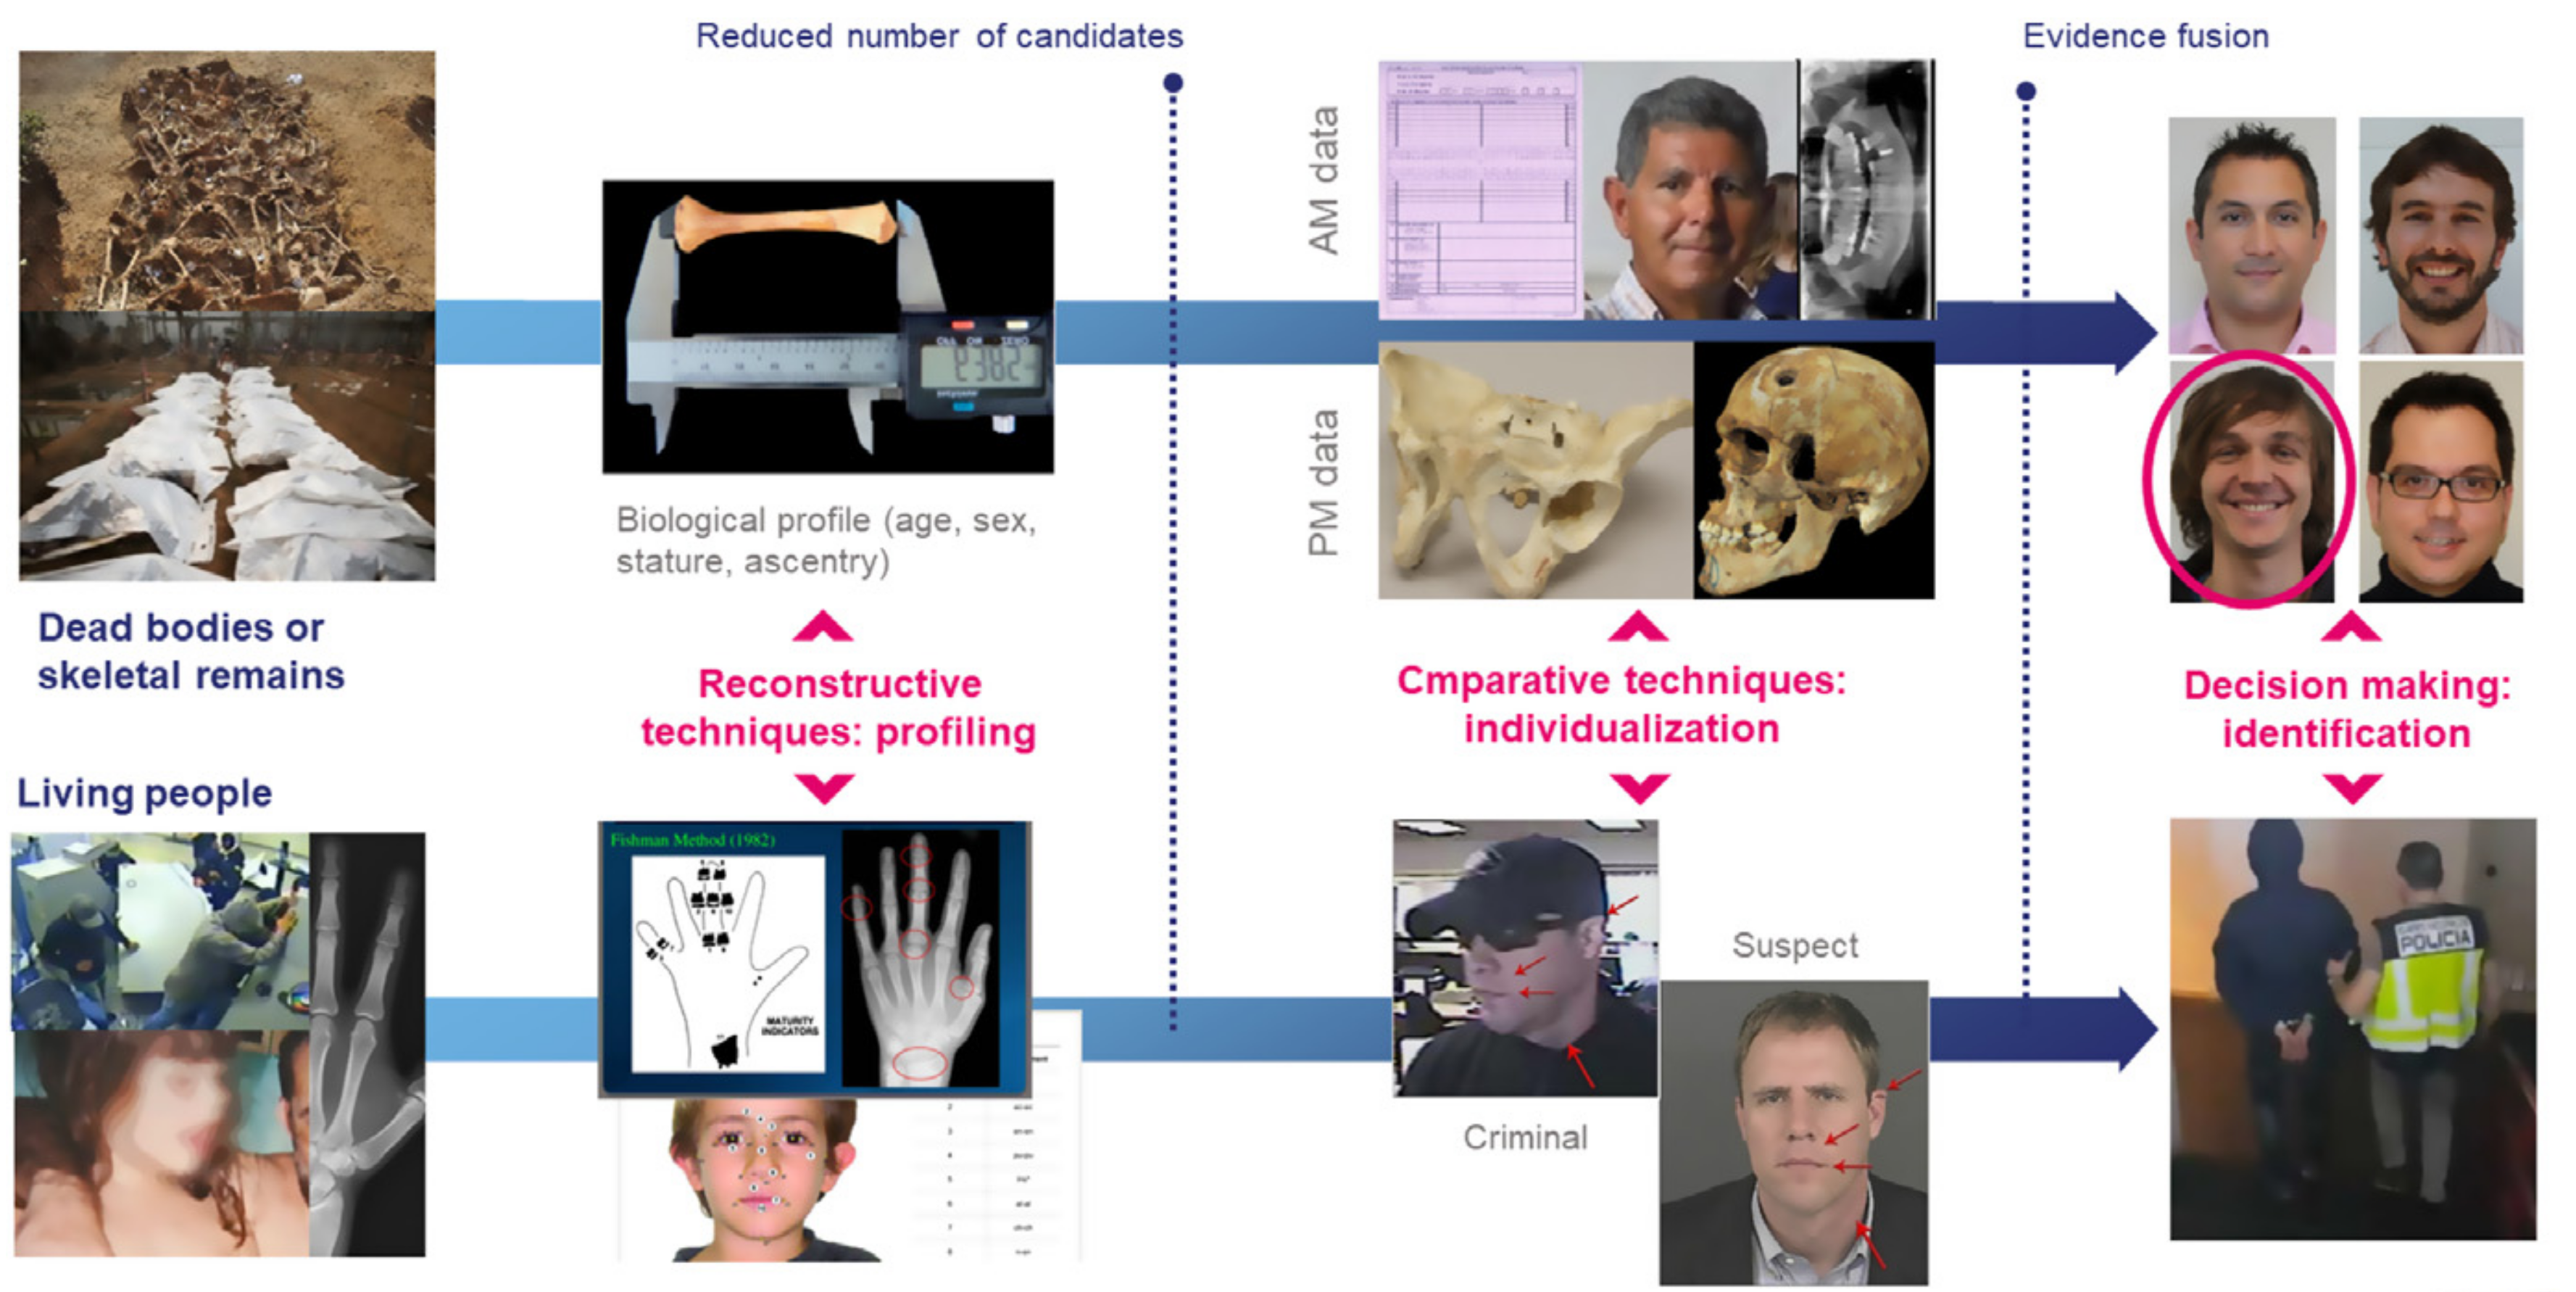
\includegraphics[width=\textwidth]{capitulos/cap_01/imagenes/SFI_pipeline.png}
    \caption{Procedimiento secuencial para la identificación forense basada en el esqueleto humano (\textit{skeleton-based forensic identification}) \cite{mesejo2020}.} 
    \label{fig:SFI_pipeline}
\end{figure}

La estimación del PB en restos humanos es una tarea compleja, especialmente cuando se estima la edad en el momento de la muerte, ya que hay diferentes métodos a aplicar dependiendo de la fase de desarrollo del individuo. Las variaciones en la morfología de los huesos son bien conocidas, pero estas no siempre ocurren al mismo tiempo en diferentes individuos, ya que no están expuestos a las mismos condiciones genéticas y del entorno.

Además, como se ha mencionado anteriormente, la estimación de edad también se realiza sobre personas vivas en casos legales donde la edad es un factor determinante \cite{schmeling2016}, por ejemplo, con menores migrantes no acompañados. En estos casos no se tiene acceso a los huesos de la persona de forma directa, por lo que el análisis se realiza sobre imágenes médicas.

% ------------------------------------------------------------------------------------------------------------
% ------------------------------------------------------------------------------------------------------------
% ------------------------------------------------------------------------------------------------------------

\section{Motivación}

Los métodos de estimación del PB se basan en la evaluación visual y en el análisis morfométrico de rasgos esqueléticos, que requieren de conocimiento especializado. Sin embargo, su aplicación puede presentar ambigüedades en su formulación que den lugar a interepretaciones variables ---muchas veces fruto de sesgos cognitivos \cite{nakhaeizadeh2014, cooper2019}--- y están sujetos a posibles errores de medición \cite{langley2018}. Además, la gran variabilidad genética y ambiental entre individuos, que afecta la morfología del esqueleto y genera diferencias significativas entre poblaciones de distintas regiones \cite{ubelaker2017}, hace que muchos de estos métodos ---basados en muestras de referencia limitadas o no representativas de la diversidad humana global--- pierdan precisión. Esto puede introducir sesgos al estimar el PB de individuos de grupos poco estudiados o con características atípicas.

Frente a estas limitaciones, recientes avances en inteligencia artificial (IA) y \textit{machine learning} (ML) han demostrado el potencial de mejorar la exactitud y objetividad de estimación del PB, tanto para la estimación de sexo \cite{curate2017, darmawan2015, pinto2016} como de edad \cite{kim2017, larson2018, lee2017}.

Sin embargo, aún mejorando la exactitud de las predicciones, los modelos siguen mostrando carencias respecto a la cuantificación de incertidumbre, pues no todas las predicciones tienen el mismo nivel de confianza o fiabilidad. Ya en \cite{ferrante2009} se introducía no solo la necesidad de identificar el método adecuado para estimar la edad a partir de los elementos disponibles, sino también de evaluar su confiabilidad y realizar un estudio del error arrojado por las predicciones del método. Estos generalmente se han basado en la estadística frecuentista%
\footnote{
    La estadística frecuentista es la corriente que se desarrolla a partir de los conceptos de probabilidad y que se centra en el cálculo de probabilidades y el contraste de hipótesis.
}
\cite{verma2020, stepanovsky2024, heinrich2024}. Un ejemplo de este tipo de análisis se ilustra en la Figura \ref{fig:regression_lentibia_stature}, donde se examina la distribución probabilística del error residual arrojado por el modelo de regresión propuesto en \cite{verma2020}.

\begin{figure}[h]
    \centering
    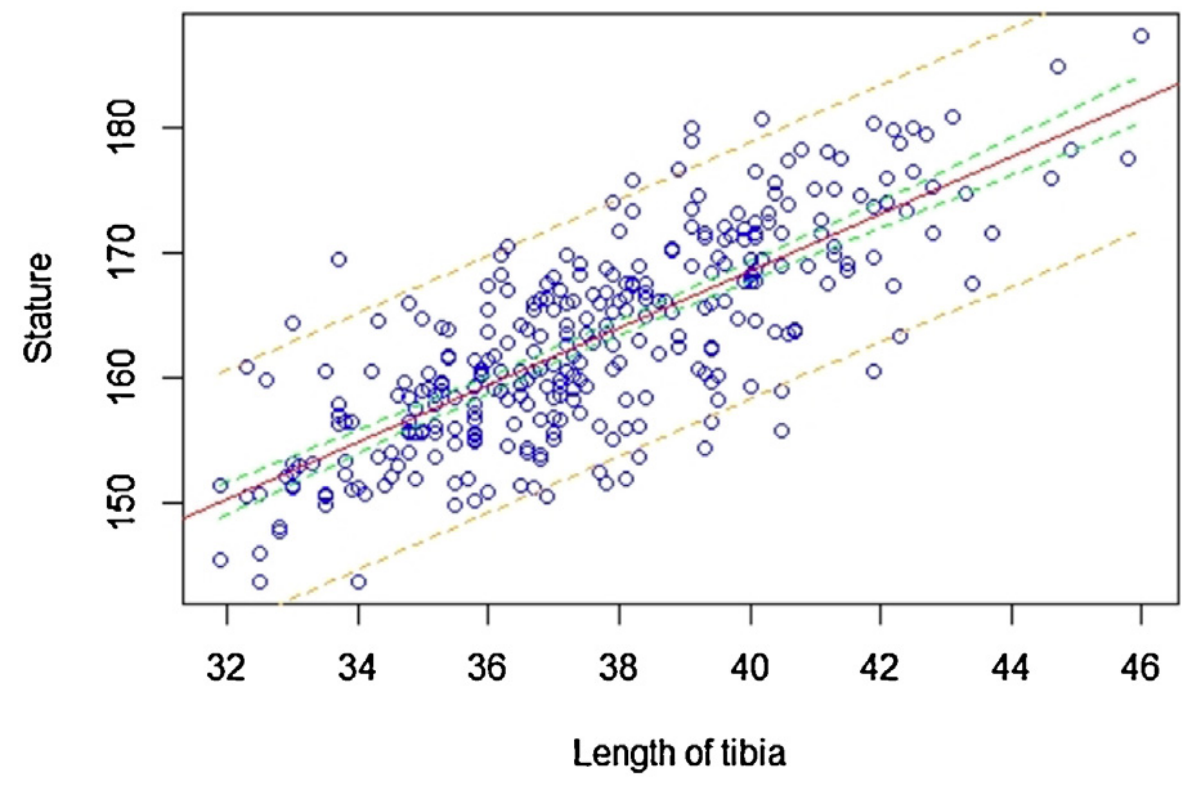
\includegraphics[width=0.7\textwidth]{capitulos/cap_01/imagenes/regression_line_lentibia_stature.png}
    \caption[
        Línea de regresión del modelo de regresión propuesto en \cite{verma2020} que predice la estatura a partir de la longitud de la tibia.
    ]{
        Línea de regresión del modelo de regresión propuesto en \cite{verma2020} que predice la estatura a partir de la longitud de la tibia. En rojo, la línea de regresión; en verde, la línea de los intervalos de confianza del 95\%; y en naranja, la línea de los intervalos de predicción al 95\% de confianza.
    } 
    \label{fig:regression_lentibia_stature}
\end{figure}

Aunque existen métricas para evaluar el error cuando se dispone de \textit{ground truth}, la mayoría de los modelos actuales se limitan a ofrecer predicciones puntuales en regresión \cite{park2024, imaizumi2021, stepanovsky2024} o etiquetas únicas en clasificación \cite{venema2022, park2024}, sin cuantificar la incertidumbre asociada a cada predicción.

Con lo anterior se expone la motivación de la aplicación de ML a la AF, así como de la necesidad de cuantificar la incertidumbre en las predicciones, para ofrecer garantías de confiabilidad estadística que aspiren a sustentar la validez legal en contextos judiciales. Algunos datos que magnifican la necesidad de técnicas de AF confiables actualmente son:

% 1/3 de los muertos del 11S sin identificar

\begin{itemize}

    \item En los últimos años, ha aumentado significativamente el número de cadáveres hallados en el territorio español, como podemos apreciar en la Figura \ref{fig:evolucion_hallazgosID_cadaveres} \cite{interior2025desaparecidos}. En 2024 se ha alcanzado una cifra record, ---en gran parte debido a las inundaciones de la DANA Valencia---, de 531 cadáveres en 2024, de los cuales se pudo identificar a 323.

    \begin{figure}[h]
        \centering
        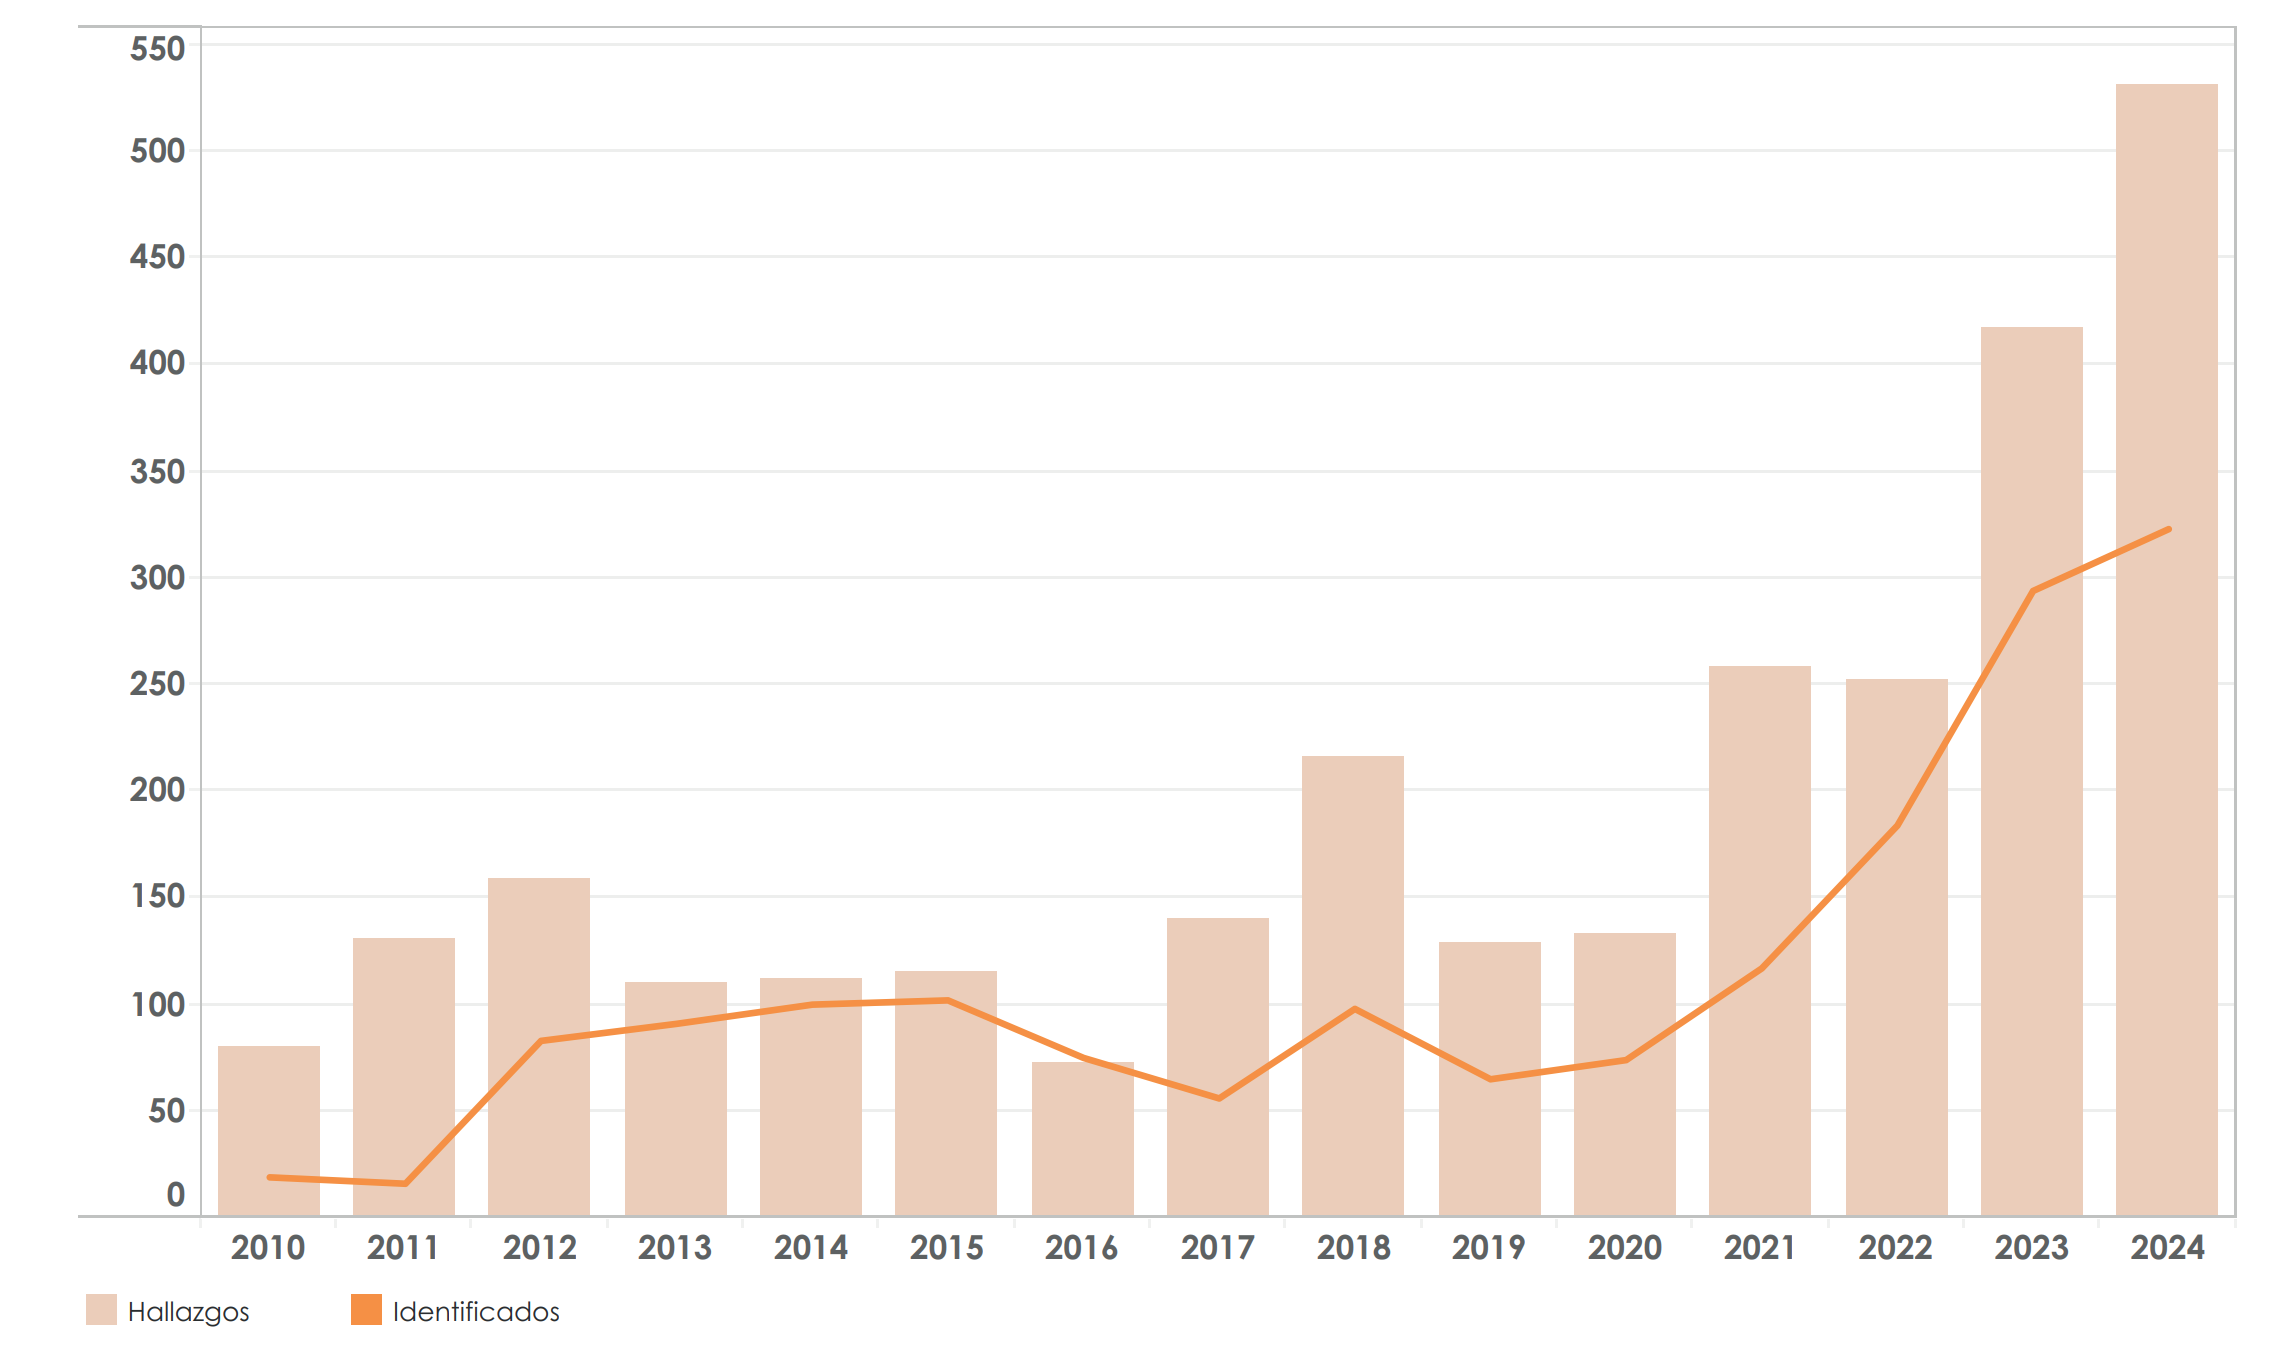
\includegraphics[width=\textwidth]{capitulos/cap_01/imagenes/hallazgos_cadaveres.png}
        \caption[
            Evolución de hallazgos/identificación de cadáveres en España (2010-2024) \cite{interior2025desaparecidos}.
        ]{
            Evolución de hallazgos/identificación de cadáveres en España (2010-2024) \cite{interior2025desaparecidos}. 
        } 
        \label{fig:evolucion_hallazgosID_cadaveres}
    \end{figure}

    \item En 2020, de las 2.457 fosas totales documentadas de la Guerra Civil y el franquismo, aún 1.221 seguían sin ser intervenidas y se estimaba que ``con una intervención oficial del Estado podrían recuperarse unos 20 a 25.000 individuos'' e identificar ``entre 5 y 7.000 de ellos'', estimándose  necesario contar con unos 40-50 profesionales de la antropología forense \cite{etxeberria2020}. 

    % \item De acuerdo con UNICEF \cite{unicef2013}, en 2012 cerca de 230 millones de niños menores de cinco años no contaban con un registro oficial de nacimiento. Las regiones con las tasas más bajas de registro incluyen África subsahariana (44\%) y el sur de Asia (39\%). Esta situación se agrava aún más, ya que muchos niños registrados no poseen un certificado de nacimiento, y los documentos existentes suelen perderse durante procesos de migración.

    \item En España, se ha registrado en la última década (2013-2023) un aumento significativo en la llegada de Menores Extranjeros No Acompañados \cite{fge2024,fge2019,fge2016,fge2013}, que ha disparado consigo el número de diligencias abiertas para la determinación de su edad, como se ve reflejado en la Figura \ref{fig:evolucion_DPDE}.

    \begin{figure}[h]
        \centering
        \includegraphics[width=\textwidth]{capitulos/cap_01/imagenes/dpde_España.png}
        \caption{
            Evolución del número de diligencias preprocesales de determinación de edad abiertas en España (2011–2023). Elaboración propia a partir de \cite{fge2013,fge2016,fge2019, fge2024}.
        } 
        \label{fig:evolucion_DPDE}
    \end{figure}

    \item La relevancia de la ciencia forense en la identificación de víctimas y la protección de la dignidad humana ha convertido su aplicación en un pilar fundamental de los derechos humanos y la justicia internacional, naciendo así la  \textbf{acción forense humanitaria} \cite{cordner2017}. Esta disciplina emplea la ciencia forense con un propósito exclusivamente humanitario, con los objetivos de: identificar a las personas fallecidas, gestionar dignamente sus restos y aliviar el sufrimiento de sus familias en situaciones de conflicto, migración y desastres naturales \cite{tidballbinz2021}. 

\end{itemize}

% ------------------------------------------------------------------------------------------------------------

\section{Objetivos}

La \textbf{predicción conformal} emerge como un marco teórico robusto para generar intervalos de predicción con garantías estadísticas sólidas, independientemente de la distribución subyacente de los datos. A diferencia de los enfoques tradicionales, este método no solo ofrece predicciones puntuales sino que cuantifica la incertidumbre asociada a cada estimación mediante intervalos o conjuntos de predicción que reflejan la confiabilidad de la predicción en cada caso particular.

Este Trabajo de Fin de Grado tiene un doble objetivo: 

\begin{itemize}

    \item desde un prisma teórico, defender la cuantificación de incertidumbre como herramienta esencial en ML, ofrecer un panorama de métodos destacados, analizando sus ventajas y limitaciones, y centrarnos en la predicción conformal y sus técnicas más populares.

    \item aplicar la predicción conformal a un contexto práctico como es el problema de estimación del PB, centrándose en la estimación de edad y de sexo a partir de datos biológicos e imágenes médicas.

\end{itemize}

De esta forma, podremos incorporar la incertidumbre propia del problema a resolver y del modelo entrenado para él, para, en aquellos casos más confusos, devolver conjuntos de predicciones con más de una etiqueta predicha (p.ej., \{masculino, femenino\}) en problemas de clasificación, o intervalos de predicción más amplios (p.ej., edad$\in$[16,20]) en problemas de regresión, en ambos casos para un nivel de confianza determinado.

Por tanto, podemos desgranar los objetivos en:

\todo{Pablo: Esto no creo que quede muy claro. Generalmente, se proponen uno o dos objetivos principales, y luego se presentan una serie de objetivos parciales, cuya consecución asegura el cumplimiento de los objetivos principales. Pero aquí no me queda claro si estos son los objetivos parciales... entiendo que sí. De ser así, no dudes en indicarlo con claridad, diciendo sin ambages que estos son objetivos parciales.}

\begin{itemize}

    \item Estudiar de forma exhaustiva la bibliografía sobre predicción conformal y sus diversas variantes, así como de la estimación de sexo y edad, centrando nuestra atención en el estado del arte.

    \todo{David: Entonces falta apartado para la estimación de sexo en el estado del arte}

    \item Implementar, entrenar y validar modelos de regresión ---en problemas de estimación de edad--- y clasificación ---tanto en problema de estimación de sexo como edad legal--- a los que aplicar la inferencia conformal.

    \item Comparar los intervalos y conjuntos de predicciones generados para evaluar su calibración empírica, robustez ante datos ambiguos y utilidad forense, contrastándolos con métodos tradicionales (p.ej., intervalos de confianza clásicos).  

    \item Realiza una primera aproximación a un marco interpretable y con garantías estadísticas para la estimación del perfil biológico (véase un ejemplo práctico en la Figura \ref{fig:example_intervalic_estimation}), donde la incertidumbre cuantificada pueda integrarse en informes periciales bajo estándares jurídicos.

\end{itemize}

% \todo{
%     Pablo: Algo que yo creo que podría ser de utilidad al lector es mostrar un esquema genérico visual de lo que piensas hacer a nivel práctico, por ejemplo, a la hora de estimar la edad empleando una red neuronal. Yo incluiría un esquema de aprendizaje automático, como la Fig. 3 de https://link.springer.com/article/10.1007/s00521-022-07981-0, pero añadiendo elementos visuales que indiquen y subrayen la idea de que se emplean intervalos de predicción (con un conjunto de calibración, por ejemplo) para cuantificar la incertidumbre en las predicciones proporcionadas.
    
%     Dicho de otro modo: queremos una figura que, de un vistazo, permita entender cómo vas a combinar estimación de la edad (por ejemplo) e intervalos de predicción (y estos últimos de dónde salen). Aunque luego los detalles se presenten más adelante, un diagrama en la introducción creo que ayudaría a aterrizar las ideas principales.
% }

\begin{figure}[h]
    \centering
    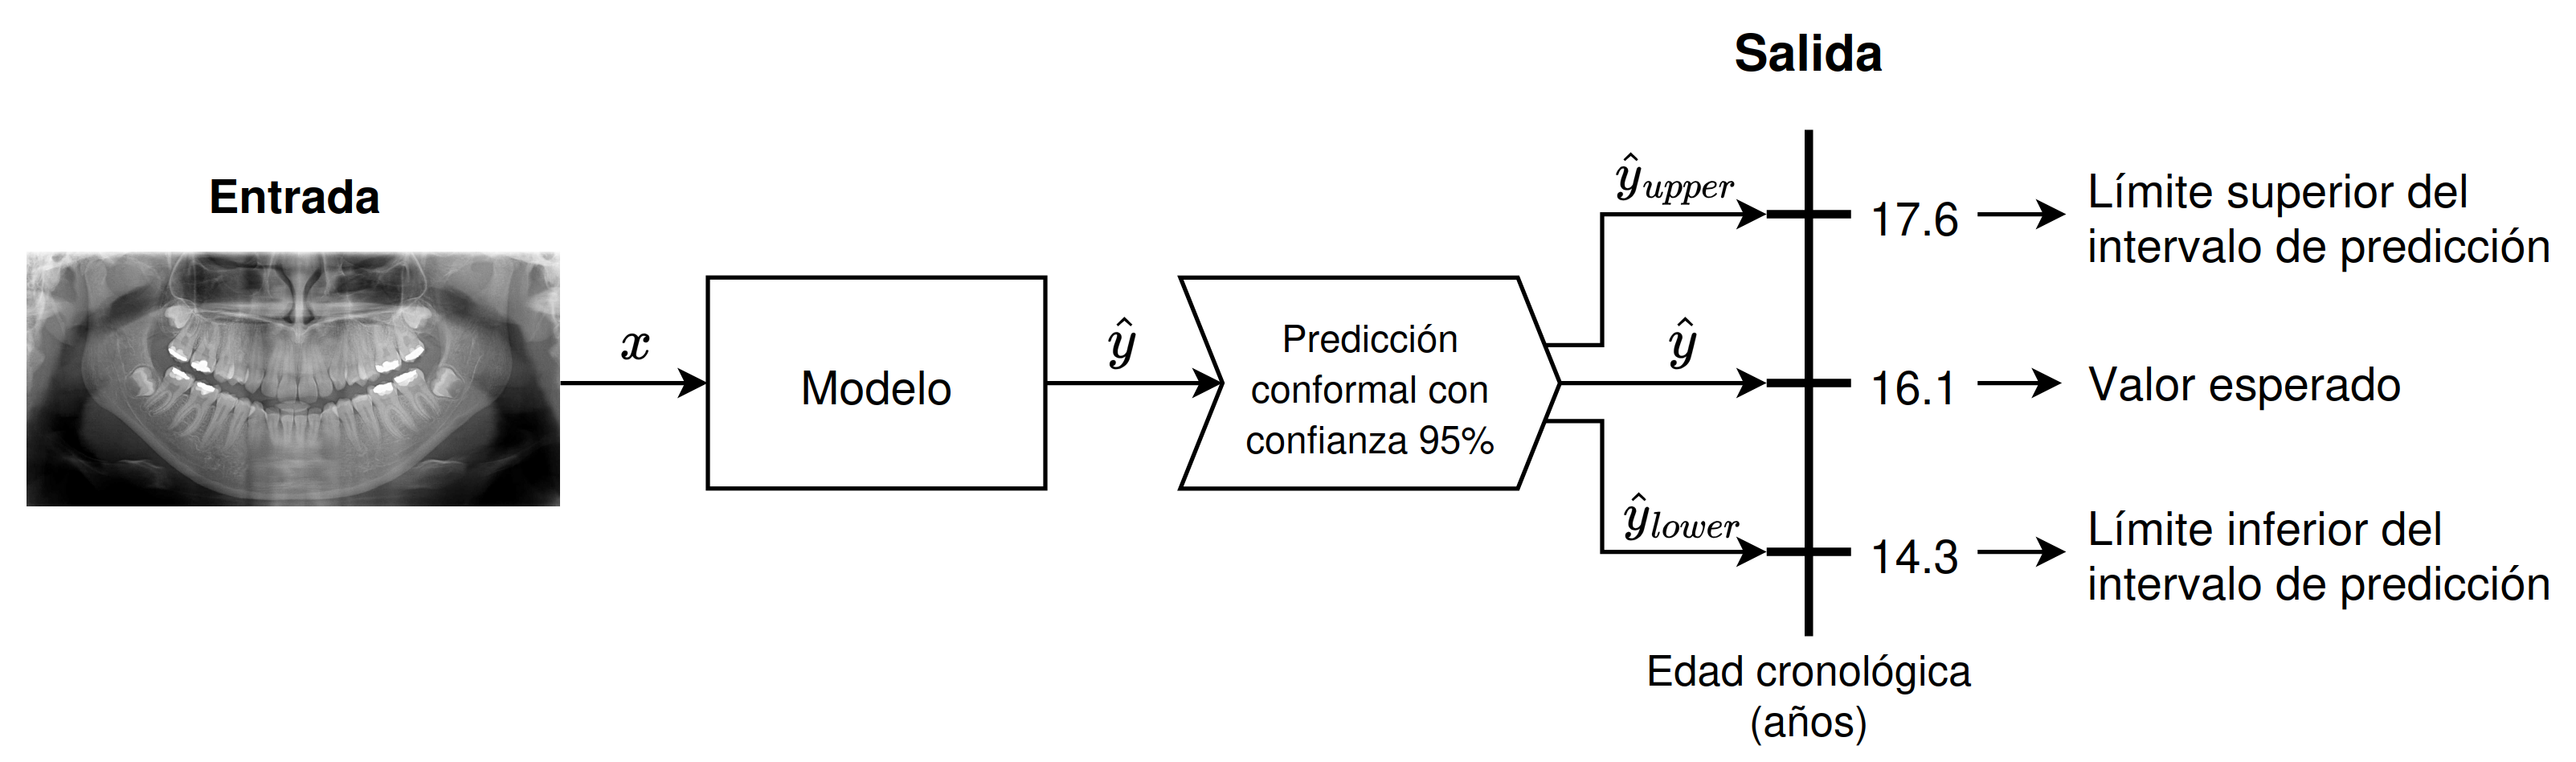
\includegraphics[width=\textwidth]{capitulos/cap_01/imagenes/example_intervalic_estimation.png}
    \caption[
        Diagrama de modelo de regresión que usa predicción conformal, el cual, además de proporcionar una estimación puntual del valor esperado, entrega un intervalo de predicción con un nivel de confianza del 95\%.
    ]{ 
        Diagrama de modelo de regresión que usa predicción conformal, el cual, además de proporcionar una estimación puntual del valor esperado, entrega un intervalo de predicción con un nivel de confianza del 95\%.
        Esta salida se lee de la siguiente manera: ``la edad esperada del individuo es de 16.1 años y, con una confianza del 95\%, la edad real del individuo está entre los 14.3 y los 17.6 años''.
    } 
    \label{fig:example_intervalic_estimation}
\end{figure}


En resumen, este trabajo pretende explorar la integración de marcos probabilísticos en la práctica forense que capturen la incertidumbre de los problemas, y facilitar el uso de la inferencia conformal en ellos. Este enfoque proporciona estimaciones calibradas de incertidumbre, con garantías estadísticas de contener el valor real en un conjunto o intervalo de predicción, útiles para la toma de decisiones fundamentadas en contextos prácticos donde la interpretabilidad y robustez son críticas.

% ------------------------------------------------------------------------------------------------------------

\section{Planificación temporal del proyecto}

\todo{Por completar (AGOSTO) con el histórico de GitHub}

% ------------------------------------------------------------------------------------------------------------

\section{Planificación económica del proyecto}

Este trabajo ha sido realizado con dos equipos independientes: 

\begin{itemize}

    \item Un ordenador portátil personal, empleado principalmente para la redacción y compilación de este documento en \LaTeX.
        
    \item Un clúster de computación proporcionado por el Instituto de Ciencia de Datos e Inteligencia Artificial (DaSCI), de la Universidad de Granada, al que se accedió mediante conexión SSH. Para el desarrollo de los distintos modelos y variantes de predicción conformal, se utilizó el entorno de desarrollo Visual Studio Code de Microsoft.

\end{itemize}

\todo{
    Pablo:La idea principal en este punto es que, al tratarse de un proyecto de ingeniería, se suele incluir una sección dedicada a la planificación. 

    Hay dos motivos para hacerlo: por un lado, es una buena práctica en sí misma (es decir, un proyecto debe ser planificado); por otro lado, satisfará (al menos parcialmente) a los miembros del tribunal más ligados a ingeniería del software. 

    Una vez dicho esto, debemos tener claro que la planificación tiene dos caras: una temporal (representada por los dos diagramas de Gantt: inicial y final, en el caso de un TFG/TFM) y una económica (qué recursos se necesitan para llevar a cabo el proyecto en cuestión; incluyendo los recursos humanos). 

    En relación a esta última parte, la planificación económica, lo que se suele hacer es incluir el coste por hora del trabajador, y dejarlo ahí. Eso suele ser criticado, con razón, por los tribunales de TFG/TFM, dado que parece lógico también presupuestar el material requerido para la realización del trabajo (licencias software, equipos hardware, etc.). En el otro extremo hay gente que presupuesta hasta los lápices... eso no se debe hacer porque suena a puteo hacia el tribunal. Pero sí es una buena práctica presupuestar los equipos que se van usar (y otros elementos de cierta enjundia que puedan ser necesarios). Por ejemplo, si tú para tus experimentos necesitas un servidor de GPU, valorado en 50K euros, debes ponerlo. Pero, ojo, no tiene sentido que digas que, para hacer tu TFG, necesitas 50K euros. Ese es el coste de todo el servidor durante toda su vida útil. Tú basta con que presupuestes un porcentaje del mismo, de modo aproximado, y correspondiente al uso que le vas a dar. Piensa, por ejemplo, en un coche. Te compras un Dacia Duster por 14K euros y a los 5 años decides venderlo. El coche ya no vale 14K euros. Lo has utilizado, se ha gastado, y ahora vale menos. Eso es a lo que se refiere con amortización. Si lo vendo por 5K euros. Se puede decir que el coste del coche para mi proyecto fue de 9K euros. 

    Comento todo esto por si te sirve de ayuda a la hora de redactar esta sección.
}

% Gasto hardware

En cuanto al software, todo el empleado es gratuito y de código abierto. 

\todo{Por completar (AGOSTO)}


   %
   %\chapter{Fundamentos teóricos}

Este capítulo tiene el propósito de presentar y describir los fundamentos teóricos que sustentan los métodos 
utilizados en el trabajo, además de justificar su importtancia para abordar los problemas planteados.

% ------------------------------------------------------------------------------------------------------------
% MACHINE LEARNING -------------------------------------------------------------------------------------------
% ------------------------------------------------------------------------------------------------------------

\section{Machine Learning}

Frente a la idea de intentar crear un programa que simulara directamente el comportamiento inteligente de una 
``mente adulta'', Alan Turing ya vaticinó un enfoque alternativo \cite{turing1950}: que las máquinas pudieran 
aprender como lo hace un niño, mediante un ``proceso educativo'' con el cual se logra alcanzar progresivamente 
una ``mente adulta'', obteniendo así comportamientos inteligentes complejos.

En los años 50, surgió el concepto de \textit{machine learning} (ML) ---o aprendizaje automático en
español---, popularizado por Arthur L. Samuel \cite{samuel1959}, para designar una rama marginal de la IA, 
centrada en el desarrollo de modelos y algoritmos que permitiesen a las 
computadoras imitar la forma en la que los humanos aprenden, realizar tareas autónomas y mejorar su 
rendimiento a través de la experiencia y exposición a más datos. De esta forma, estos modelos podrían realizar 
predicciones o tomar decisiones sin ser programados para cada caso.

En las décadas de 1960, 1970 y 1980, surgieron algoritmos fundamentales como el perceptrón 
\cite{mcculloch1943,rosenblatt1958} o los árboles de decisión \cite{quinlan1986}, 
que sentaron los cimientos teóricos para el desarrollo posterior de técnicas más complejas.  
Sin embargo, el progreso fue lento debido a las limitaciones computacionales y el gran escepticismo académico. 

Los años 90 y 2000 marcaron un punto de inflexión para el ML, gracias a los avances teóricos, el mayor poder 
computacional y la disponibilidad de grandes volúmenes de datos. De 2010 en adelante, la evolución del ML ha 
sido exponencial, marcada por la consolidación del \textit{deep learning}, la escalabilidad masiva y su 
integración en numerosas aplicaciones: de visión por computador, reconocimiento de lenguaje natural, robótica, 
diagnóstico médico y forense, finanzas o recomendación de contenidos, entre otros. De esta forma, el ML se ha 
convertido en un campo tan amplio y exitoso que ahora ``eclipsa'' al resto de campos de la IA 
\cite{domingos2015}.

El ML diferencia tres tipos de aprendizaje en base a tres tipos de retroalimentación \cite{rusell2021}: 

\begin{itemize}
    
    \item \textbf{Aprendizaje supervisado}, en el que el agente (refiriéndose con este al modelo de ML y su 
    algoritmo de aprendizaje) observa ejemplos de pares entrada-salida y aprende la función que mejor mapea 
    las entradas (inputs) a las salidas (outputs) correspondientes. El objetivo es generalizar este 
    aprendizaje para hacer predicciones precisas sobre datos nuevos y no vistos \cite{bishop2006}.

    \item \textbf{Aprendizaje por refuerzo}, en el que los datos de entrenamiento no contienen salida 
    objetivo, sino que contiene posibles resultados junto con medidas de calidad de dicho resultado, es decir, 
    una función de evaluación del estado. En este tipo de aprendizaje, el agente toma decisiones en un entorno 
    y recibe recompensas o penalizaciones por las acciones que realiza, ajustando su comportamiento mediante 
    prueba y error, maximizando la recompensa acumulada en el tiempo \cite{alpaydin2010}.

    \item \textbf{Aprendizaje no supervisado}, en el que el agente tampoco dispone de valores de salida, solo 
    de entrada \cite{bishop2006}, y los objetivos pueden ser muy variados, centrándose en descubrir patrones, 
    estructuras o relaciones ocultas en los datos. A diferencia de los otros enfoques, aquí no hay una 
    ``respuesta correcta'' predefinida, sino que el modelo debe inferir conocimiento directamente desde la 
    distribución de los datos.

\end{itemize}

Este trabajo se centrará en el aprendizaje supervisado, pues es este tipo de aprendizaje el empleado en los 
problemas de clasificación y regresión que aplicaremos en el ámbito de la antropología forense.

El objetivo en el aprendizaje supervisado es establecer una hipótesis que se ajuste de forma óptima a los
ejemplos futuros. Para ello, se presupone que los ejemplos futuros mostrarán un comportamiento similar a los
pasados. Bajo este supuesto, el ajuste óptimo de un modelo es, por tanto, la hipótesis que minimiza la tasa
de error del problema \cite{rusell2021}.


% Retos en el aprendizaje supervisado


% No importa el formato de entrada



% ------------------------------------------------------------------------------------------------------------

% En el \textbf{aprendizaje supervisado} \cite{bishop2006}, el agente (refiriéndose con este al 
% modelo de ML y su algoritmo de aprendizaje) observa ejemplos de pares entrada-salida y aprende
% la función que mejor mapea las entradas (inputs) a las salidas (outputs) correspondientes. El 
% objetivo es generalizar este aprendizaje para hacer predicciones precisas sobre datos nuevos y 
% no vistos.

% Hay dos principales tipos de problemas de aprendizaje supervisado: 

% \begin{itemize}
%     \item la \textit{clasificación} para cuando el valor de salida es una etiqueta categórica, y
%     \item la \textit{regresión} cuando el valor de salida es un valor continuo.
% \end{itemize}

% % ----------------------------------------------------------------------------------------------------------

% En cambio, en el \textbf{aprendizaje por refuerzo}, los datos de entrenamiento no contienen 
% salida objetivo, sino que contiene posibles resultados junto con medidas de calidad de dicho 
% resultado, es decir, una función de evaluación del estado. En este tipo de aprendizaje, el 
% agente toma decisiones en un entorno y recibe recompensas o penalizaciones por las acciones 
% que realiza, ajustando su comportamiento mediante prueba y error, maximizando la recompensa 
% acumulada en el tiempo \cite{alpaydin2010}.  

% De esta forma, el algoritmo no aprende a dar una acción/salida a partir de un input, sino que 
% desarrolla una política que determina la mejor acción a tomar en cada estado del entorno, con 
% el objetivo de maximizar la recompensa acumulada a largo plazo.

% Esta aproximación es clave en aplicaciones como juegos, robótica, optimización de recursos y 
% sistemas conversacionales (ChatAI), donde las decisiones secuenciales y la interacción 
% dinámica con el entorno son fundamentales.

% % ----------------------------------------------------------------------------------------------------------

% Y, por último, en el \textbf{aprendizaje no supervisado}, el agente tampoco dispone de valores 
% de salida, solo de entrada \cite{bishop2006}, y los objetivos pueden ser muy variados, 
% centrándose en descubrir patrones, estructuras o relaciones ocultas en los datos. 

% A diferencia de los otros enfoques, aquí no hay una "respuesta correcta" predefinida, sino que 
% el modelo debe inferir conocimiento directamente desde la distribución de los datos.

% Algunos problemas clásicos de este tipo de aprendizaje son: 

% \begin{itemize}

%     \item El \textit{clustering} o agrupamiento, donde el objetivo es encontrar clústeres o 
%     agrupaciones del input. Esto puede ser útil, por ejemplo, para una empresa que quiera 
%     segmentar sus clientes, o para identificar patrones en datos genéticos sin etiquetar.
    
%     \item La \textit{detección de anomalías} (\textit{outlier detection} en inglés), que 
%     consiste en encontrar instancias atípicas o inusuales en los datos. Sus aplicaciones 
%     incluyen: identificación de fraudes en transacciones bancarias, fallos en equipos 
%     industriales o identificación de ciberataques.

%     \item La \textit{reducción de dimensionalidad}, que trata de reducir el número de 
%     variables manteniendo la mayor información posible. Esto es útil para visualizar datos 
%     complejos o mejorar la eficiencia de algoritmos (p.ej., transformaciones PCA y t-SNE).

%     \item El \textit{aprendizaje de representaciones} (como los \textit{autoencoders}), 
%     donde el modelo busca capturar características latentes de los datos de manera eficiente. 
%     La compresión de archivos o la reducción de ruido en imágenes son algunos ejemplos de 
%     aplicaciones. 

% \end{itemize}



% ------------------------------------------------------------------------------------------------------------

\subsection{Problemas de regresión}

Como se ha mencionado antes, la regresión es un tipo de problema clásico en el aprendizaje supervisado, y 
consiste en predecir el valor de una o más \textbf{variables continuas} objetivo a partir de unos datos de 
entrada \cite{bishop2006}, utilizando un modelo entrenado con ejemplos ya con valores conocidos.

Matemáticamente, este proceso implica modelar la relación entre la variable dependiente $Y$ y las variables
independientes $X$, de modo que se pueda predecir o explicar el comportamiento de $Y$ en función de los 
valores de $X$. El modelo aprende una función de predicción $f$ que, dado un nuevo ejemplo $i$ con 
características $X_i$, genera una estimación $\hat{Y_i}$:

$$
f(X_i) = f(X_{i0}, X_{i1}, \dots, X_{in}) = \hat{Y_i} = Y_i + \varepsilon_i
$$

donde 

\begin{itemize}
    \item $X_{i0},X_{i1}, \dots, X_{in}$ son las características o atributos del ejemplo $i$,
    \item $Y_i$ es el valor real de la variable objetivo para ese ejemplo,
    \item $\hat{Y_i}$ es la predicción generada por el modelo, y
    \item $\varepsilon_i$ representa el error o residuo 
    \footnote{
        A pesar de que en la literatura más especializada ---que veremos a continuación---, los términos 
        ``error'' y ``residuo'' se distinguen. 
    }, 
    es decir, la diferencia entre la predicción y el valor real.
    Este término captura factores aleatorios o imprecisiones que el modelo no logra explicar perfectamente.
\end{itemize}

El análisis y la evaluación estadística del error son fundamentales para valorar la utilidad práctica del 
modelo y optimizar su capacidad predictiva mediante técnicas de ajuste y validación.

% ------------------------------------------------------------------------------------------------------------

\subsection{Problemas de clasificación}

En cambio, en los problemas de clasificación, los valores de salida son categóricos, denominados más 
comúnmente como \textbf{clases}, y a cada valor individual asignado a una instancia de datos se le conoce como 
\textbf{etiqueta} (\textit{label} en inglés).

Existen multitud de variante de clasificación, que pueden diferenciarse según diversos criterios:

\begin{itemize}
    \item En base a la cardinalidad de las clases de salida: \textbf{clasificación binaria o multiclase}, 
    según si existen dos clases posibles o más de dos, respectivamente.

    \item En base al número de etiquetas asignadas a cada instancia: \textbf{clasificación con etiqueta única 
    o multietiqueta}, según si cada instancia pertenece a una sola clase o a varias de forma simultánea.

    \item En base a la certeza de la asignación de clases: \textbf{clasificación con etiqueta precisa o 
    difusa}, donde en el primer caso la asignación a una clase es determinista, y en el segundo caso se 
    permite una pertenencia parcial a varias clases, con distinto grados de afinidad.
    
\end{itemize}

No obstante, la mayoría de los problemas estudiados en la literatura de ML, y concretamente en antropología 
forense, corresponden a clasificación binaria o multiclase, con etiquetas únicas y asignación precisa 
\cite{bishop2006}, que serán el foco de este trabajo. La cardinalidad de las clases tiene implicanciones 
significativas en el diseño del modelo y la evaluación de su desempeño:

\begin{itemize}

    \item \textbf{Clasificación binaria}, que es aquella en la que existen únicamente dos clases posibles para 
    la variable objetivo, siendo común en problemas donde se desea discriminar entre dos estados mutuamente 
    excluyentes (p.ej., ``positivo'' vs. ``negativo'', ``spam'' vs. ``no spam'', ``fraude'' vs. ``no 
    fraude'').
    
    Se suele denominar a una de las clases como ``positiva'' y a otra como ``negativa'' para facilitar la 
    interpretación de métricas como la precisión, la sensibilidad o la especifidad, si bien no tiene por qué 
    existir una connotación valorativa entre ambas clases.
    
    \item \textbf{Clasificación multiclase}: en este caso, la variable objetivo puede tomar más de dos valores 
    posibles, pertenecientes a un conjunto finito. Un ejemplo de problema clásico es el de clasificar dígitos
    manuscritos (0-9).

\end{itemize}

En este tipo de problemas, el error ocurre cuando no se acierta al predecir la clase del ejemplo.

% Tanto en clasificación binaria como multiclase, un problema común es el desequilibrio de clases, donde una 
% clase tiene muchos más ejemplos que otra. Esto afecta el entrenamiento del modelo, ya que puede sesgarse 
% hacia la clase mayoritaria, ya que el modelo





% ------------------------------------------------------------------------------------------------------------
% ENSEMBLE LEARNING ------------------------------------------------------------------------------------------
% ------------------------------------------------------------------------------------------------------------

% \section{Ensemble Learning}

% El \textbf{aprendizaje por conjuntos (\textit{ensemble learning})} es una familia de técnicas de ML que 
% combina múltiples modelos de aprendizaje automático ---denominados \textbf{modelos base}--- para obtener un 
% modelo final con un mejor desempeño que los modelos base por separado.

% \subsection{Bagging}


% \subsection{Boosting}


% \subsection{Stacking}


% ------------------------------------------------------------------------------------------------------------
% DEEP LEARNING ----------------------------------------------------------------------------------------------
% ------------------------------------------------------------------------------------------------------------

\section{Deep Learning}

El \textbf{aprendizaje profundo (\textit{deep learning}, DL)} es una familia de técnicas de ML que utilizan 
múltiples capas de procesamiento para aprender representaciones de datos con varios niveles de abstracción
\cite{lecun2015}. Las redes neuronales han demostrado ser especialmente eficaces para este propósito, al 
permitir la composición jerárquica de características que capturan patrones cada vez más complejos en los 
datos.

Las redes neuronales tienen su origen en el intento de modelar las redes de neuronas del cerebro humano 
\cite{mcculloch1943}. Se requirió de numerosas contribuciones teóricas ---como el perceptrón 
\cite{rosenblatt1958} o el algoritmo de \textit{backpropagation} \cite{rumelhart1986,werbos1994}, entre 
otras---, disponibilidad de datos estandarizados y un gran aumento en la capacidad computacional para poder 
escalar estar redes y obtener resultados 
sorprendentes en tareas complejas.

Las \textbf{redes neuronales profundas (\textit{deep neural networks}, DNNs)} destacan por su capacidad para 
aprender representaciones jerárquicas: cada capa extrae características progresivamente más abstractas 
\cite{lecun2015}, desde líneas en imágenes hasta formas geométricas complejas, objetos completos e incluso 
escenas compuestas.
Esta propiedad las hace excepcionalmente versátiles, ya que procesan datos de muy diversa naturaleza ---datos 
tabulares, imágenes, audio, texto o señales temporales---, dados que ellas mismas aprenden los procesos de 
extracción de características de estos, hasta ahora realizados ``a mano'' (mediante procesos diseñados por la 
ingeniería de características) \cite{rusell2021} 
\footnote{
    Este enfoque se denomina aprendizaje extremo a extremo (\textit{end-to-end learning}), en el cual tanto la 
    extracción de características como la clasificación son parte de un modelo integral que se entrena de 
    manera conjunta, optimizando todos los componentes del sistema en un mismo proceso \cite{rusell2021}.
}. 
Gracias a ello, las DNNs han alcanzado rendimientos sobresalientes en dominios como visión por computador 
(clasificación de imágenes, detección de objetos, segmentación) o procesamiento de lenguaje natural 
(traducción, generación de texto) \cite{redhat2024DeepLearningDefinition}.
No obstante, su eficacia depende críticamente de grandes volúmenes de datos y recursos computacionales, lo que 
ha impulsado técnicas como el \textit{transfer learning} y modelos eficientes para democratizar su uso.


\subsection{El perceptrón multicapa}

El \textbf{perceptrón multicapa (\textit{multilayer perceptron}, MLP)} forma la base del \textit{deep 
learning}. Su diseño ---con capas ocultas, funciones de activación no lineales y entrenamiento  mediante 
\textit{backpropagation}--- sentó las bases conceptuales para arquitecturas más complejas, como las redes 
neuronales convolucionales o los \textit{transformers} \cite{murphy2022}. El MLP sigue siendo un referente 
teórico y la expresión más simple de cómo el aprendizaje jerárquico puede capturar patrones en los datos. 

Cada nodo en la red es denominado \textbf{unidad o neurona artifical}. Siguiendo el diseño propuesto en 
\cite{mcculloch1943,rosenblatt1958}, cada unidad recibe señales de entrada ---que o bien son las 
características de los datos o bien las salidas de las unidades de la anterior capa---, realiza una suma 
ponderada de estas con los pesos entrenables de cada conexión ---más un término independiente o sesgo, también 
entrenable---, aplica una función no lineal sobre esta para producir una salida que propaga a las unidades de 
la siguiente capa (véase la Figura \ref{fig:neuron_MLP}).

Matemáticamente, la operación de una unidad artifical se expresaría como:

$$
y = f \left( \sum_{i=1}^n{w_ix_i+b} \right)
$$

donde $x_i$ son las entradas, $w_i$ son los pesos entrenables ($w_0$ el sesgo)
\footnote{
    El sesgo se considera un peso, puesto que, en la implementación, son un peso más conectado a una unidad
    de sesgo con valor constante unitario (1).
}
, y $f$ es la función de activación.

\begin{figure}[h]
    \centering
    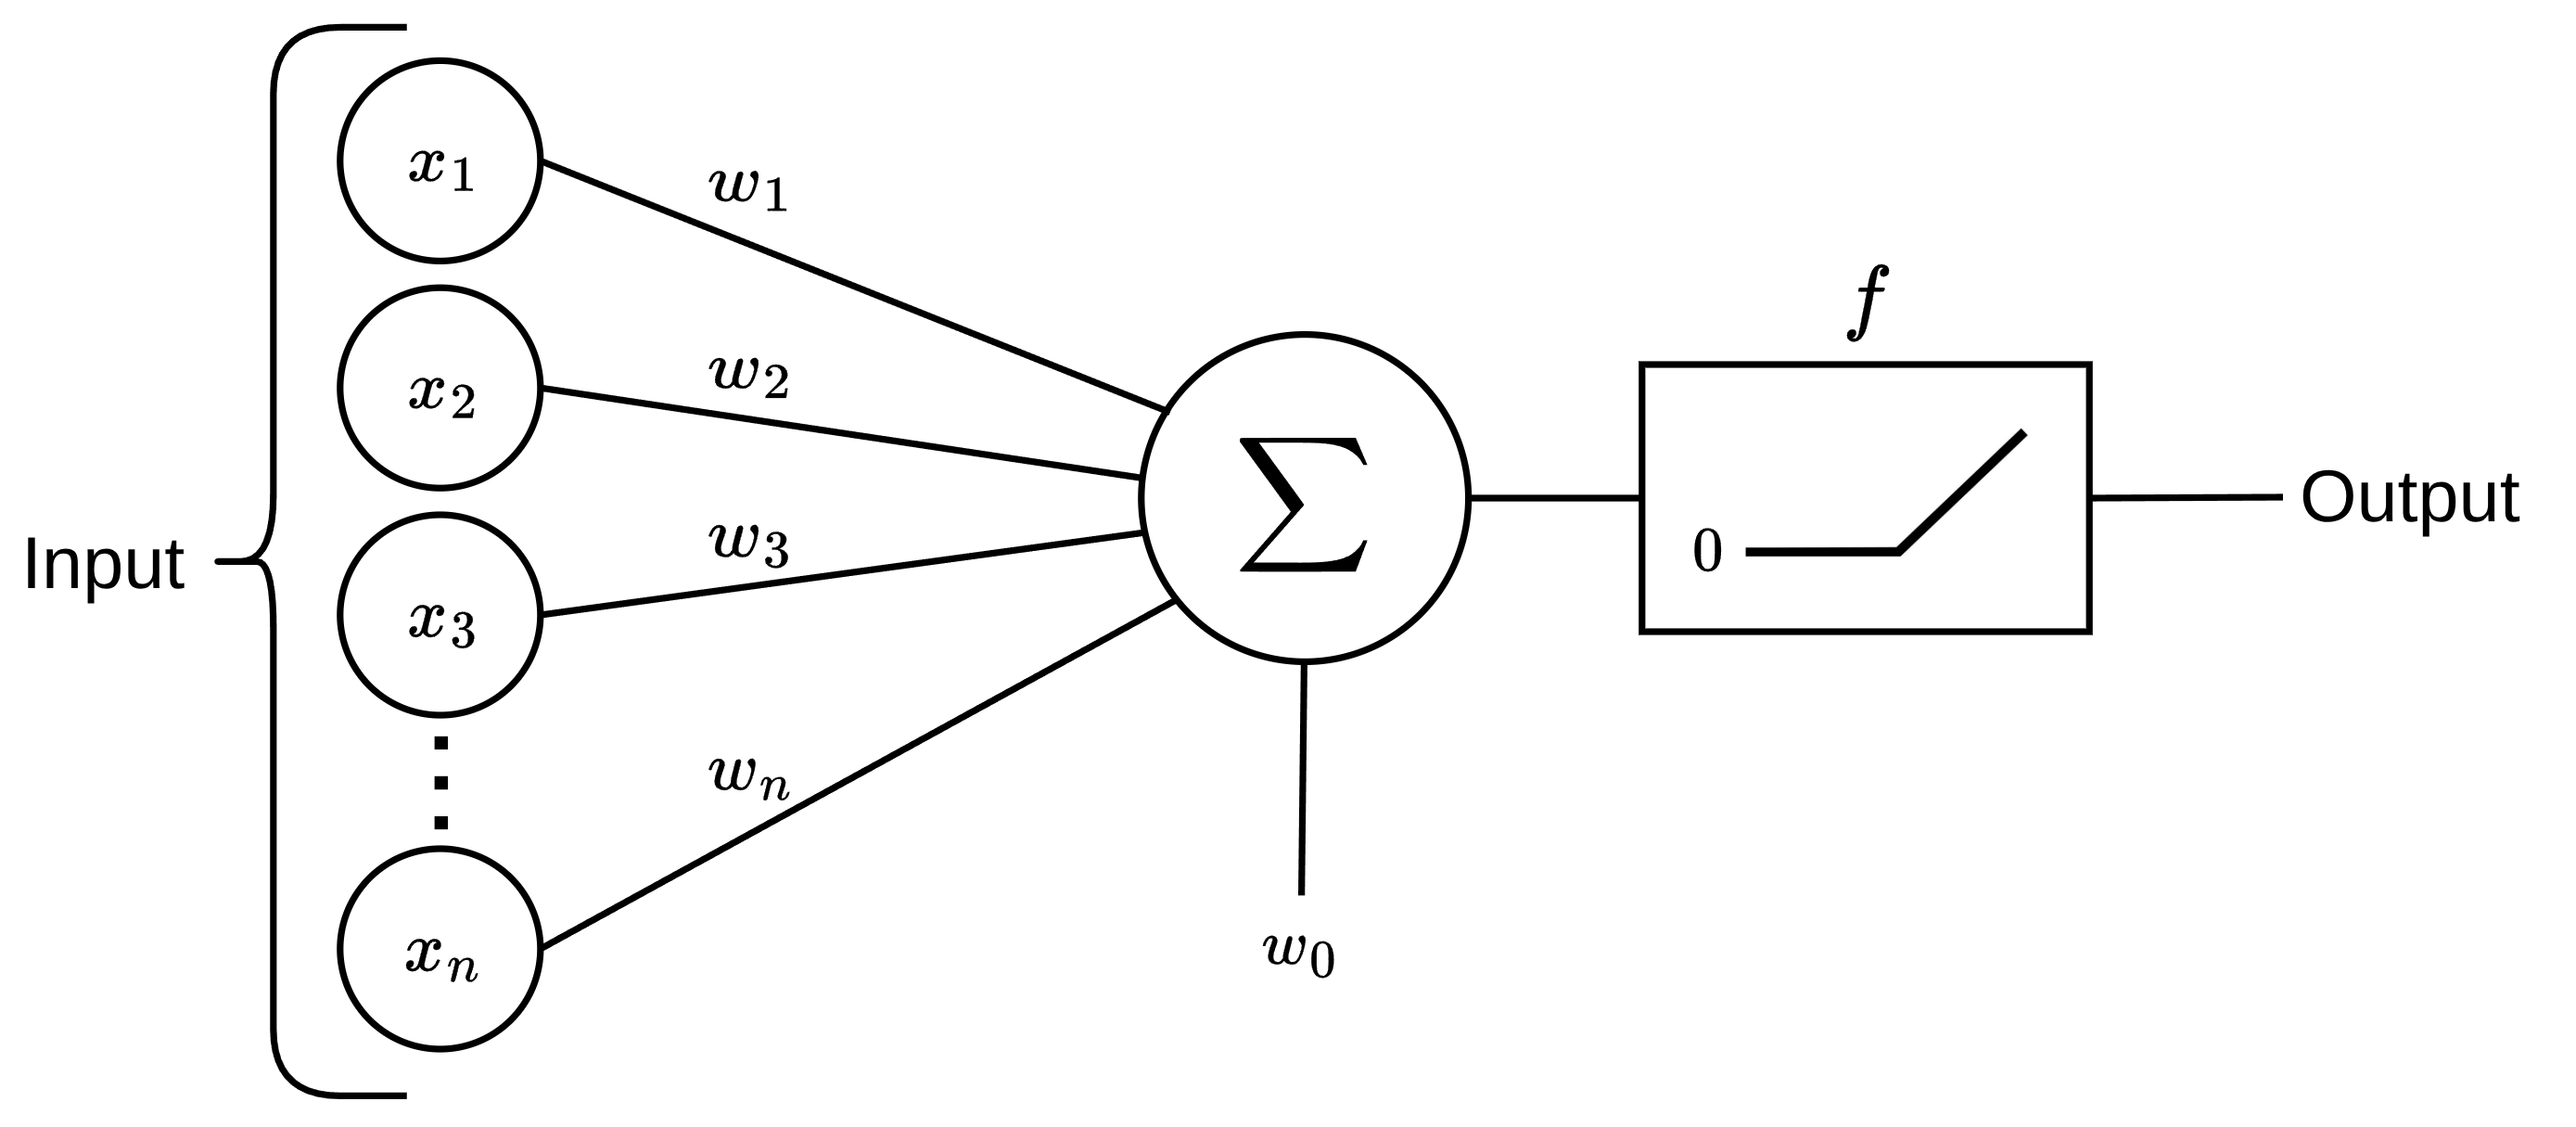
\includegraphics[width=0.95\textwidth]{capitulos/cap_02/imagenes/Neuron_perceptron.png}
    \caption{
        Esquema visual del funcionamiento de una unidad artificial. Adaptado de 
        \cite{codeworld2022understandingMLDL}.
    } 
    \label{fig:neuron_MLP}
\end{figure}


Esta \textbf{función de activación} a la salida de la unidad es un componente esencial que introduce no 
linealidad en el modelo, permitiendo a la red aprender relaciones complejas en los datos
\footnote{
    Sin ella, el MLP se reduciría a una simple combinación lineal de las entradas, incapaz de
    representar jerarquías de características \cite{murphy2022}.
}.
Existe multitud de funciones de activación, como la sigmoide, la tangente hiperbólica o ReLu ---y sus 
múltiples variantes---, cada una con sus ventajas y limitaciones
\footnote{
    Si bien, actualmente, ReLU y sus variantes (\textit{Leaky} ReLU, \textit{Parametric ReLU} o 
    \textit{Swish}) se han convertido en el estándar \textit{de facto} para las capas ocultas en DNNs,
    por su eficiencia computacional, y su eficacia empírica \cite{vargas2021}.
}.

La arquitectura de un MLP conecta estas unidades formando una red neuronal retroalimentada
\footnote{
    Una red neuronal retroalimentada (\textit{feed-forward neural network}) es aquella en la que las 
    conexiones entre las unidades no forman un ciclo y, por tanto, la información solo se mueve en una 
    dirección: adelante.
},
que consta de tres partes (véase la Figura \ref{fig:neural_network}):

\begin{itemize}

    \item \textbf{Capa de entrada}, en las que el número de unidades debe coincidir con el formato de entrada 
    de los datos, por ejemplo: en un problema con datos tabulares, debería haber una unidad por cada 
    característica.
    
    \item \textbf{Capas ocultas}, donde se realizan las transformaciones no lineales de los datos. Es en estas 
    donde el diseño puede variar en número de unidades y tipo de capas según la complejidad del problema y los 
    datos.
    
    \item \textbf{Capa de salida}, que proporciona el resultado del modelo. Su forma depende del problema a 
    resolver: 
    
    \begin{itemize}
        
        \item en problemas de regresión, esta capa tendrá tantas unidades como variables a predecir ---sin 
        función de activación, ya que esto limitaría el rango de valores posibles---;
        
        \item en problemas de clasificación, esta capa tendrá una sola unidad ---generalmente, con activación 
        sigmoide--- en clasificación binaria, o múltiples unidades ---con activación 
        \textit{softmax}
        \footnote{
            La activación \textit{softmax} no se aplica sobre la salida de una única unidad, sino que se 
            aplica sobre un vector de salidas de múltiples unidades, transformándolas en una distribución de 
            probabilidad, donde cada valor representa la probabilidad de pertenecer a una clase distinta y la 
            suma de todas las salidas es igual a 1.
        }
        --- en clasificación multiclase (véase la Figura \ref{fig:activation_func_classification}).
    \end{itemize}

\end{itemize}

\begin{figure}[h]
    \centering
    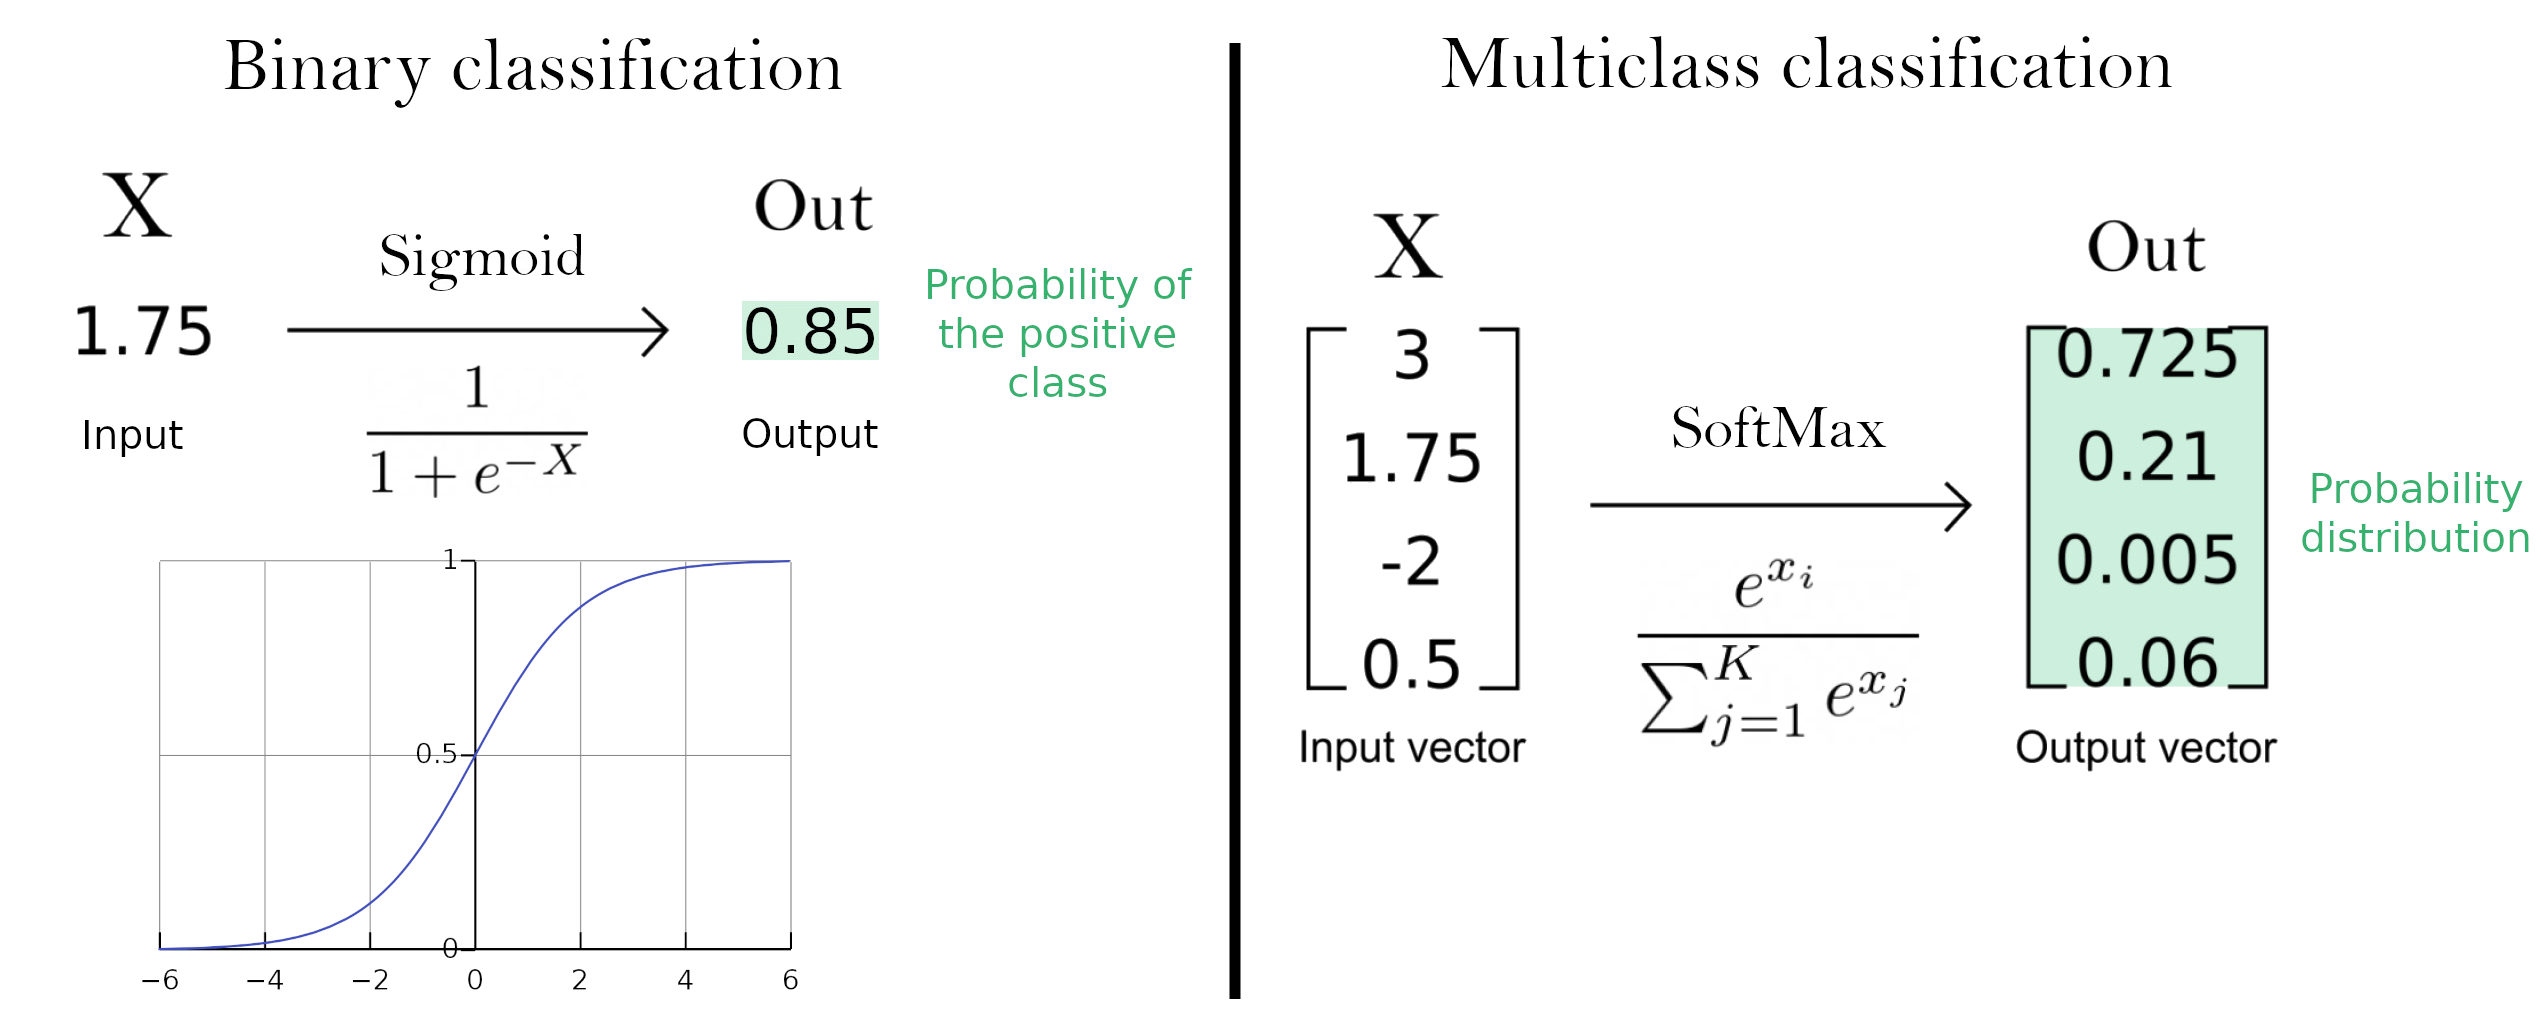
\includegraphics[width=\textwidth]{capitulos/cap_02/imagenes/ActivationFuncClassification.png}
    \caption{
        Diagrama de obtención de probabilidad en problemas de clasificación. 
        Adaptado de \cite{furnieles2022sigmoidandsoftmax}.
    } 
    \label{fig:activation_func_classification}
\end{figure}

%Quitar X y Out, y subir lo de abajo

\begin{figure}[h]
    \centering
    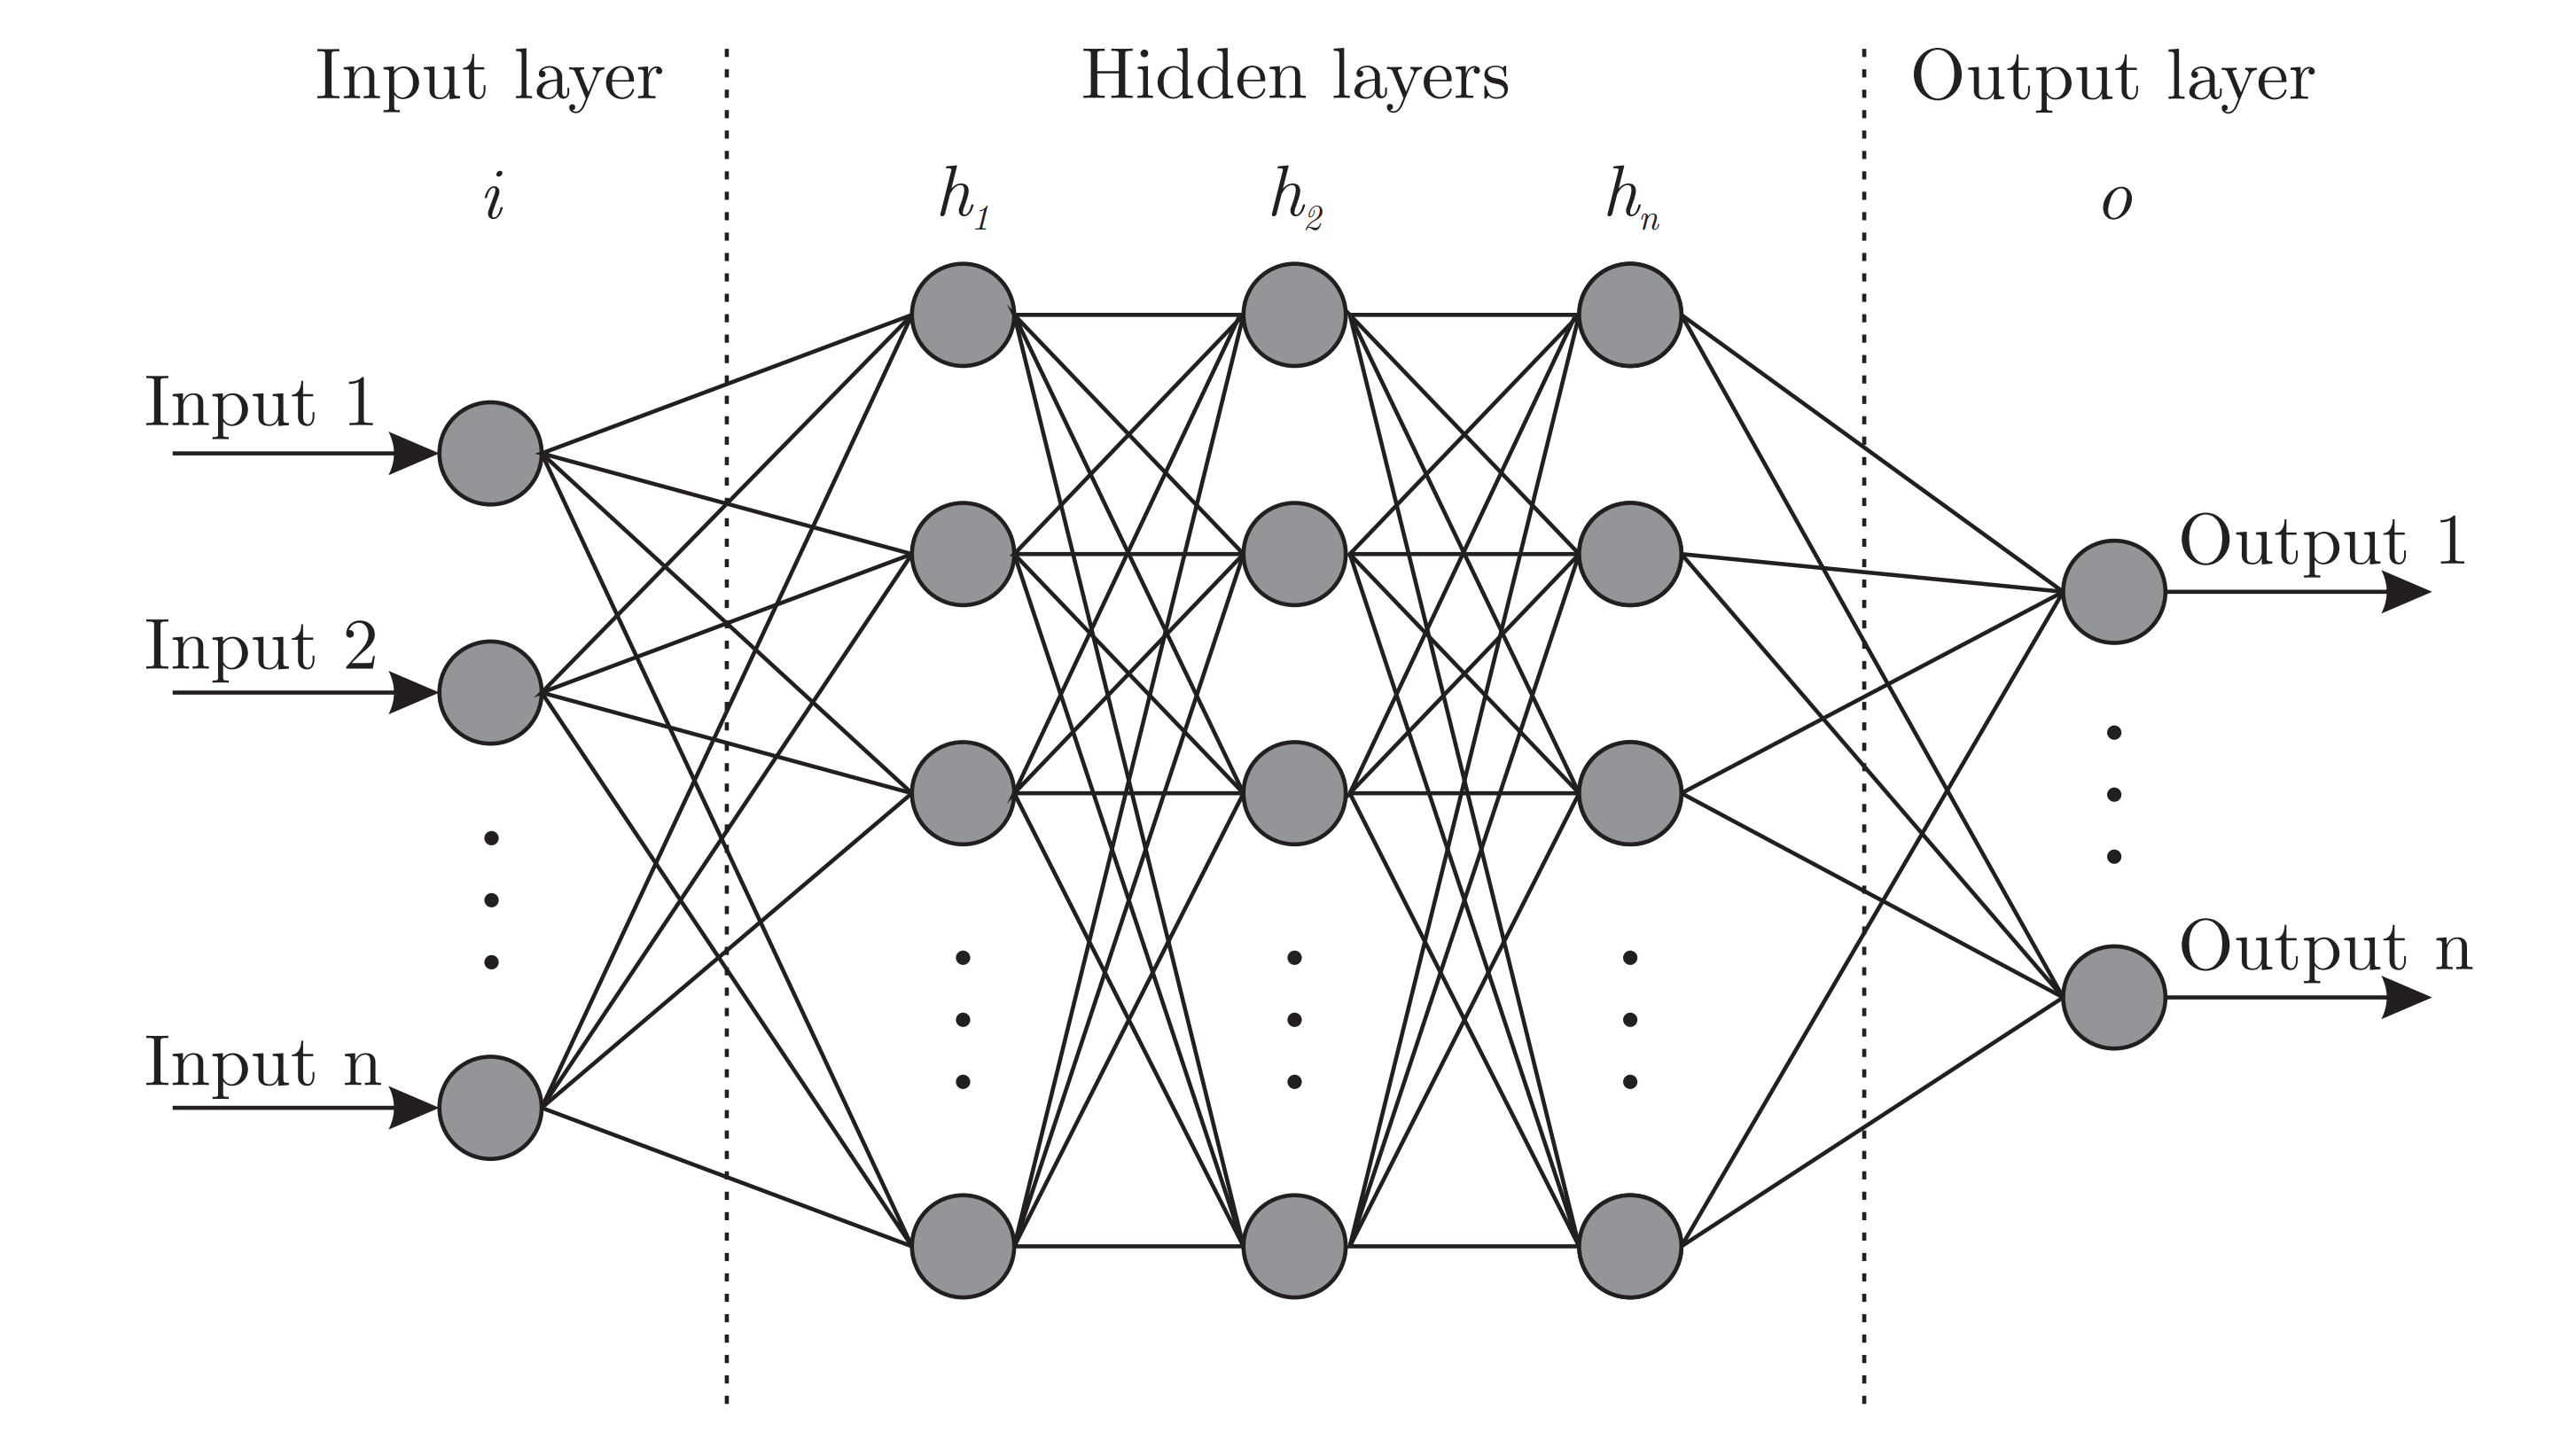
\includegraphics[width=0.95\textwidth]{capitulos/cap_02/imagenes/neural_network.png}
    \caption{
        Arquitectura simplificada de un MLP. 
        Recuperado de \cite{bre2017}.
    } 
    \label{fig:neural_network}
\end{figure}

% ------------------------------------------------------------------------------------------------------------

\subsection{Entrenamiento y validación de la red}

En el caso de las redes neuronales, el conjunto de datos suele dividirse en tres 
subconjuntos: entrenamiento, validación y prueba. A diferencia de métodos más tradicionales, no se utiliza 
validación cruzada, ya que entrenar redes profundas conlleva un elevado coste computacional.

Una vez hemos definido la arquitectura a emplear para resolver un problema, y definido los datos disponibles 
debemos entrenar la red con los datos de ejemplo. Este proceso implica ajustar los pesos del modelo para 
minimizar el error en las predicciones. 

El método de entrenamiento estándar en redes neuronales es el \textbf{algoritmo de retropropagación 
(\textit{backpropagation})}, que funciona en dos fases clave \cite{szeliski2010}:

\begin{itemize}

    \item \textbf{Propagación hacia adelante (\textit{forward pass})}: Los datos de entrada se procesan a 
    través de las capas de la red, generando una predicción. 

    \item \textbf{Propagación del error hacia atrás (\textit{backward pass})}: El error entre la 
    predicción y el valor real se calcula y se propaga hacia atrás en la red, ajustando los pesos mediante el 
    descenso de gradiente.
    
    Sin entrar en demasiado detalle, esto consiste en calcular el gradiente de la función de pérdida con           % Esto de "sin entrar en demasiado detalle" qué tal? 
    respecto a cada peso de la red, indicando cómo cada parámetro contribuye al error total. 
    A mayor aporte al error de un peso, más se ajustará ese peso. Así, el algoritmo priorizará modificar 
    significativamente los parámetros que más afectan al rendimiento de la red.
    
\end{itemize}

Este proceso explicado de manera vaga, tiene infinidad de detalles y variantes que influyen en su eficiencia y
eficacia:

\begin{itemize}

    \item El error obtenido entre la predicción y el valor real se calcula mediante la \textbf{función de 
    pérdida (\textit{loss function})}. Esta función cuantifica el error del modelo durante el entrenamiento, 
    midiendo la discrepancia entre las predicciones generadas y los valores o clases reales (\textit{ground 
    truth}).

    No se debe confundir con las métrica de evaluación de un modelo: aunque en algunos casos se pueden usar 
    métricas como funciones de pérdida y viceversa, las métricas destacan por ser fáciles de interpretar 
    y suele utilizarse más de una. En cambio, debe existir una únifa función de pérdida durante el 
    entrenamiento de una red neuronal, que debe cumplir tres requisitos clave:

    \begin{enumerate}

        \item Reflejar el objetivo del aprendizaje: Debe capturar adecuadamente qué significa ``éxito'' para 
        el modelo (p.ej., minimizar el error en regresión o maximizar la probabilidad de clasificación 
        correcta).

        \item Ser diferenciable: Es esencial para aplicar técnicas de descenso por gradiente, ya que el 
        optimizador necesita calcular derivadas.

        \item Ser eficiente computacionalmente: Dado que se evalúa en cada iteración del entrenamiento, su 
        cálculo debe ser rápido incluso con grandes volúmenes de datos.

    \end{enumerate}

    Mientras las métricas ayudan a entender el modelo, la función de pérdida es la que lo entrena.

    En problemas de regresión se emplean funciones de pérdida como el error cuadrático medio (\textit{mean 
    squared error}, MSE), que mide la diferencia promedio al cuadrado entre las predicciones y los valores 
    reales, o el error absoluto medio (\textit{mean absolute error}, MAE), que calcula la diferencia promedio 
    en valor absoluto
    \footnote{
        Aunque esta no es derivable en $x=0$, se define la derivada en ese punto como 0.
    }.

    En clasificación, las funciones de pérdida más comunes son la entropía cruzada (\textit{cross-entropy 
    loss}) para problemas de clasificación binaria y multiclase, que penaliza fuertemente las predicciones 
    incorrectas y ayuda a optimizar las probabilidades predichas para cada clase.


    \item Existen multitud de \textbf{algoritmos de optimización de parámetros}, como SGD, Adam o RMSProp. 
    Estos algoritmos determinan cómo actualizar los pesos del modelo durante el entrenamiento para minimizar 
    la función de pérdida. 
    Están basados en el descenso de gradiente, que ajusta los pesos en dirección opuesta al gradiente de 
    la función de pérdida respecto a los pesos, multiplicado por un factor escalar llamado \textbf{tasa 
    de aprendizaje (\textit{learning rate})}. Este hiperparámetro controla la magnitud de los pasos de 
    actualización: un valor demasiado alto puede hacer que el entrenamiento diverja, mientras que uno 
    demasiado bajo ralentiza la convergencia o estanca el modelo en mínimos locales.

    Existen estrategias avanzadas para ajustar el \textit{learning rate} de manera más eficiente durante el 
    entrenamiento, como la búsqueda de un \textit{learning rate} de punto de partida 


    \item Si bien existen métodos de entrenamiento de redes ejemplo a ejemplo ---como el Gradiente Descendente 
    Estocástico (SGD) puro\cite{bottou2010}---, estas se suelen entrenar por lotes 
    (\textit{minibatches})
    \footnote{
        Se denomina \textit{batch} al \textit{dataset} completo, y \textit{minibatch} a los subconjuntos de
        este cuyo tamaño está determinado por el hiperparámetro \textit{batch size}.
    } 
    debido a ventajas clave, como el aprovechamiento de la paralelización de operaciones en GPU y una mayor 
    estabilidad en la función de pérdida al promediarse el error entre varios ejemplos. 
    Aún así, establecer un tamaño de lote óptimo no es una tarea trivial que requiere de encontrar un 
    equilibrio entre generalización y velocidad: los lotes grandes aceleran el entrenamiento pero pueden 
    reducir la generalización del modelo, mientras que los lotes pequeños puede presentar una gran varianza 
    que introduzca ruido en el modelo \cite{keskar2017}, si bien esto puede ayudar a escapar de mínimos 
    locales, y puede paliarse con un bajo \textit{learning rate} (aunque esto aumentaría todavía más los 
    tiempos de entrenamiento).
    

    \item Tras el uso de \textit{minibatches} en el entrenamiento, surge el concepto de \textbf{época 
    (\textit{epoch})}, que hace referencia a un ciclo completo de presentación de todos los datos de 
    entrenamiento a la red neuronal \cite{rusell2021}. Durante una época, los \textit{minibatches} se procesan 
    secuencialmente, actualizando los pesos del modelo en cada iteración (o \textit{step}) con el gradiente 
    calculado sobre un lote. Por ejemplo, si un conjunto de entrenamiento tiene 4096 ejemplos y el tamaño de 
    lote es 32, una época constará de 128 iteraciones (4096/32).

    El número de épocas es un hiperparámetro crítico: demasiadas pueden llevar a sobreajuste 
    (\textit{overfitting}), donde el modelo memoriza los datos de entrenamiento pero no generaliza bien; 
    demasiado pocas pueden resultar en infraajuste (\textit{underfitting}), donde el modelo no captura los 
    patrones subyacentes. Además, la combinación de tamaño de lote y épocas influye en la dinámica de 
    optimización, ya que lotes más pequeños requieren más pasos por época, introduciendo más ruido pero 
    potencialmente mejorando la exploración del espacio de pesos.

    En la práctica, se suele establecer un número muy alto de épocas, y monitorizar el error en un conjunto de
    validación para determinar cuándo detener el entrenamiento, evitando así el sobreajuste cuando el error de
    validación comienza a aumentar. A esta técnica se le denomina \textbf{\textit{early stopping}} 
    \cite{goodfellow2016}.
    
\end{itemize}


% ------------------------------------------------------------------------------------------------------------

\subsection{Redes Neuronales Convolucionales}

Como ya se venía anticipando, la arquitectura MLP es especialmente adecuada para trabajar con datos 
estructurados o tabulares, donde la información se organiza en una matriz en la que cada columna representa 
una característica concreta (como sexo, altura o peso). 
Sin embargo, su diseño presenta limitaciones clave: al manejar vectores de entrada de tamaño fijo y carecer 
de mecanismos para aprovechar relaciones espaciales o secuenciales, no es óptima para datos no estructurados, 
como imágenes o texto, donde cada elemento individual (un píxel o una palabra) carece de significado por sí 
mismo \cite{murphy2022}.

Por ejemplo, los patrones aprendidos en una posición de una imagen podrían no ser reconocidos en otra 
ubicación, ya que las entradas tienen un recorrido distinto dentro de la red. Por tanto, el modelo carecería       % DUDA: Esto de que las entradas tienen un recorrido distinto en la red se entiende?
de \textbf{invarianza traslacional}, puesto que los pesos no se comparten entre distintas posiciones, a lo que 
se suma una marcada ineficiencia por el elevado número de parámetros requeridos \cite{szeliski2010}.

Precisamente para estos casos, otras arquitecturas profundas resultan más apropiadas.
Las \textbf{redes neuronales convolucionales (\textit{Convolutional Neural Network} en inglés, CNNs)} son un 
tipo de DNN que, aprovechando las ventajas de las operaciones convolucionales, explotan los principios de 
localidad y correlación espacial. Esto les permite procesar imágenes (en 1D, 2D o 3D) de manera eficiente, 
interpretando patrones visuales jerárquicos que un MLP no podría capturar, y con significativamente menos 
parámetros.


\subsubsection{Capas convolucionales}

Como se ha introducido antes, el operador de \textbf{convolución} es la base de las CNNs. Este operador 
matemático aplica un \textbf{filtro} (también denominado \textit{kernel})
\footnote{
    Aunque, como veremos a continuación, filtro y \textit{kernel} a la hora de hablar de capas 
    convolucionales, no son técnicamente lo mismo.
} 
a regiones locales de una imagen de entrada, realizando un producto punto
\footnote{
    El producto punto o producto escalar de dos vectores, se define como la suma de los productos componente a 
    componente. 
    $$
    \mathbf{u} \cdot \mathbf{v} = \mathbf{u}_1 \cdot \mathbf{v}_1 + \mathbf{u}_2 \cdot \mathbf{v}_2 + ... + 
    \mathbf{u}_n \cdot \mathbf{v}_n
    $$
} 
entre los valores del filtro y los píxeles correspondientes de la imagen, y sustituyendo el valor del pixel 
central por el resultado del producto (véase la Figura \ref{fig:conv_op}).

\begin{figure}[h]
    \centering
    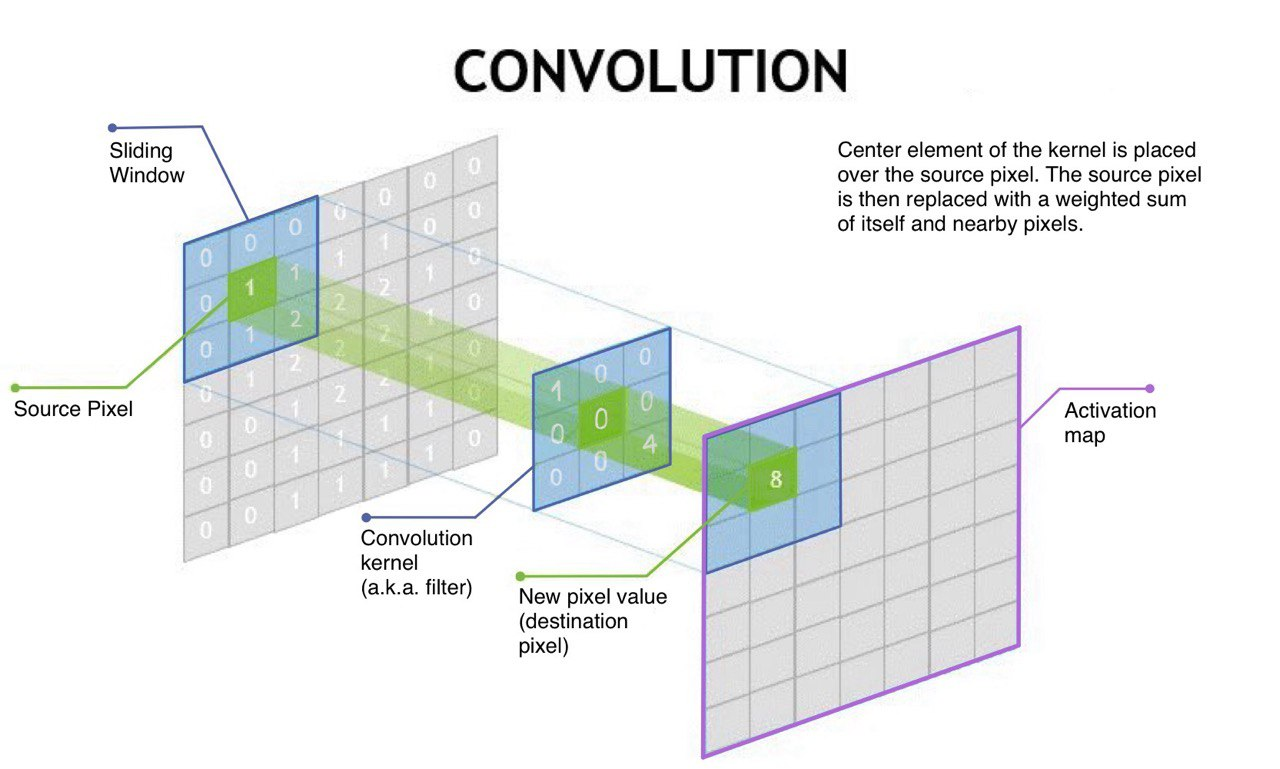
\includegraphics[width=0.95\textwidth]{capitulos/cap_02/imagenes/convolution_operation.jpg}
    \caption[Esquema gráfico de la aplicación de un filtro convolucional sobre una región de una imagen.]{
        Esquema gráfico de la aplicación de un filtro convolucional sobre una región de una imagen.
        Adaptado de \cite{nvidia2025convolutionoperation}.
    } 
    \label{fig:conv_op}
\end{figure}

Este proceso se repite al desplazar el filtro por toda la imagen mediante una \textbf{ventana deslizante}, 
generando un \textbf{mapa de activación}, que permite destacar líneas, curvas o texturas simples. Este mapa de
activación preserva la información de la localización de las características, si bien estas pueden ser 
detectadas en cualquier parte de la imagen. Esta propiedad se conoce como \textbf{equivarianza}. 

Las CNNs aprovechan la convolución mediante \textbf{capas convolucionales}. Cada capa convolucional está
compuesta por un conjunto de filtros convolucionales, donde cada uno a su vez tiene tantos \textit{kernels} 
como canales de entrada de la imagen haya en la capa (si es la primera capa convolucional, habrá 1 canal en 
imágenes de escala de grises, o 3 en imágenes RGB). El número de filtros en cada capa, su tamaño y la forma
en que se deslizan sobre la entrada
\footnote{                                                                      
    Definidos mediante los parámetros de \textit{stride} y \textit{padding}, que controlan el desplazamiento       
    del filtro y la cantidad de relleno alrededor de la entrada, respectivamente.
}
se determinan durante el diseño de la red, mientras que los valores de los \textit{kernels} son parámetros 
entrenables.

Cada filtro convolucional realiza la operación convolucional sobre cada canal con el \textit{kernel} que le 
corresponde. Después, se suman los mapas de activación de cada canal (pixel a pixel) añadiendo un sesgo 
(un mismo valor a todos los píxeles
\footnote{
    Es por ello que no rompe la propiedad de equivarianza.
}),
generando lo que denominamos como \textbf{mapa de características} (ya que idealmente extrae 
características relevantes). Los mapas de características generados con cada uno de los filtros son los nuevos 
canales, que conforman la salida de la capa convolucional. Esta salida puede ser posteriormente procesada por 
otras capas, permitiendo a la red aprender representaciones jerárquicas cada vez más abstractas de los datos 
de entrada: las primeras capas convolucionales detectarán bordes, cambios de color o texturas básicas; a 
medida que avanzamos en las capas de la red, las combinaciones de estas características simples permite 
identificar formas más complejas, como objetos e incluso composiciones.

Sin embargo, hemos pasado por alto algo fundamental: ¿cómo reunimos la información de dos regiones distantes 
de una imagen en un mismo sitio? Una primera aproximación intuitiva nos diría que los filtros convolucionales 
deben ser progresivamente más grandes, para capturar patrones de mayor tamaño y contexto. No obstante, esto
incrementaría considerablemente el número de parámetros y, por tanto, aumentaría el coste computacional y 
el riesgo de sobreajuste del modelo (ya que un modelo con más parámetros puede memorizar mejor los
datos de entrenamiento). Es por esto que, en aquellos problemas en los que no es necesario preservar la 
información de localización de las características, ---como en los que nos enfocamos en este trabajo: 
clasificación y regresión---, y, por tanto, el modelo sea invariante a la ubicación, se emplean técnicas de 
submuestreo (\textit{downsampling}) \cite{murphy2022}, como usar \textit{stride} mayor de 1 en los filtros
de las capas convolucionales o realizar \textit{pooling}
\footnote{
    Nos centraremos en el último dado su amplio uso y fácil comprensión, además de su demostrada efectividad 
    empírica.
}.



\subsubsection{Capas de pooling}

Las \textbf{capas de agrupación (\textit{pooling layers})} tienen como objetivo principal comprimir la 
información de la imagen, reduciendo sus dimensiones (alto y ancho) mientras se preservan los datos más 
relevantes para la tarea. Esta reducción del tamaño espacial de los mapas de características disminuye el 
número de parámetros y operaciones en las fases posteriores, lo que reduce el coste computacional. Además, 
tiene un beneficio adicional: ayuda a prevenir el sobreajuste, ya que al limitar la cantidad de parámetros, 
el modelo evita memorizar ruido o detalles irrelevantes de los datos de entrenamiento, favoreciendo así el 
aprendizaje de patrones generalizables.

Hay diversos métodos de \textit{pooling}, entre los que destacan:

\begin{itemize}

    \item \textbf{Max pooling}, que calcula el máximo valor de regiones del mapa de características, y lo
    usa para crear un mapa de características reducido (véase la Figura \ref{fig:max_pooling}).

    \item \textbf{Average pooling}, que reemplaza el valor máximo del \textit{max pooling} por el cálculo de
    la media entre los valores de la región. 

\end{itemize}

La región de aplicación del \textit{pooling}, al igual que en la convolución, viene determinada por ciertos 
parámetros, definidos por el diseñador, como el tamaño de filtro (que suele ser de 2x2), el \textit{stride} 
y el \textit{padding}, si bien también existen variantes  adaptativas (\textit{adaptive}), que ajustan
automáticamente su cobertura para producir una salida con dimensiones específicas, independientemente del 
tamaño de la imagen de entrada. Esta funcionalidad es especialmente útil cuando se necesita adaptar los mapas
de características para conectarlos a una capa \textit{fully-connected}. 

\begin{figure}[h]
    \centering
    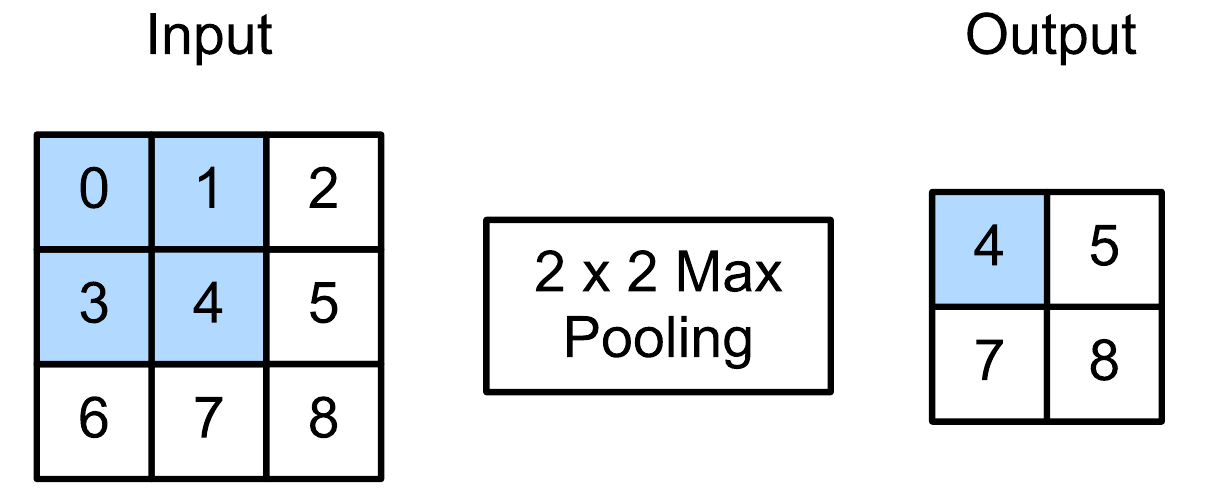
\includegraphics[width=0.7\textwidth]{capitulos/cap_02/imagenes/max_pooling.png}
    \caption{
        Esquema gráfico de \textit{max pooling} con un filtro 2x2 y \textit{stride} de 1.
        Recuperado de la Figura 14.12 de \cite{murphy2022}.
    } 
    \label{fig:max_pooling}
\end{figure}



\subsubsection{Capas \textit{Fully-Connected}}

Como hemos visto hasta ahora, en las CNNs, las primeras capas están diseñadas para extraer características
espaciales a través de filtros convolucionales y de \textit{pooling}. Sin embargo, una vez que se ha reducido 
la dimensionalidad y se han obtenido representaciones abstractas de alto nivel, es necesario realizar una 
predicción (en problemas de clasificación y regresión). 
Aquí es donde las \textbf{capas completamente conectadas (\textit{fully-connected}, FC)} juegan un papel 
crucial. Se utilizan en las últimas etapas de la red convolucional para combinar todas las características 
extraídas y producir una predicción final. Es decir, actúan como el clasificador/regresor
\footnote{
    Si bien, independientemente de la tarea ---regresión o clasificación---, a esta parte de la red se le 
    denomina clasificador
} 
que toma todas las señales procesadas por las capas anteriores y predice la clase a la que pertenece la imagen 
o el valor objetivo. 

La arquitectura de esta capa sigue la estructura del MLP, con neuronas organizadas en una o más capas densas, 
donde cada neurona está conectada con todas las salidas de la capa anterior. Para que esto sea posible, 
primero se aplica una operación de \textbf{\textit{flattening}} que transforma el mapa de características 
multidimensional en un vector unidimensional. A partir de ahí, el procesamiento es equivalente al de una red 
neuronal tradicional: cada neurona calcula una combinación lineal de sus entradas seguida de una función de 
activación no lineal.


\subsubsection{Diseño de la CNN para problemas de clasificación y regresión}

Un patrón común de diseño de CNNs para la resolución de problemas de clasificación y regresión consta de dos
componentes principales:

\begin{itemize}

    \item el \textit{backbone} o extractor de características, que alterna capas convolucionales con capas de
    \textit{pooling}, cuya función es extraer representaciones jerárquicas y cada vez más abstractas de los 
    datos de entrada; y

    \item el \textit{classifier}, generalmente implementado mediante una o más capas FC, 
    toma estas representaciones para realizar la tarea específica de salida, ya sea clasificación o regresión.

\end{itemize}

En la Figura \ref{fig:CNN_complete} se puede observar un ejemplo de arquitectura CNN completa. 


\begin{figure}[h]
    \centering
    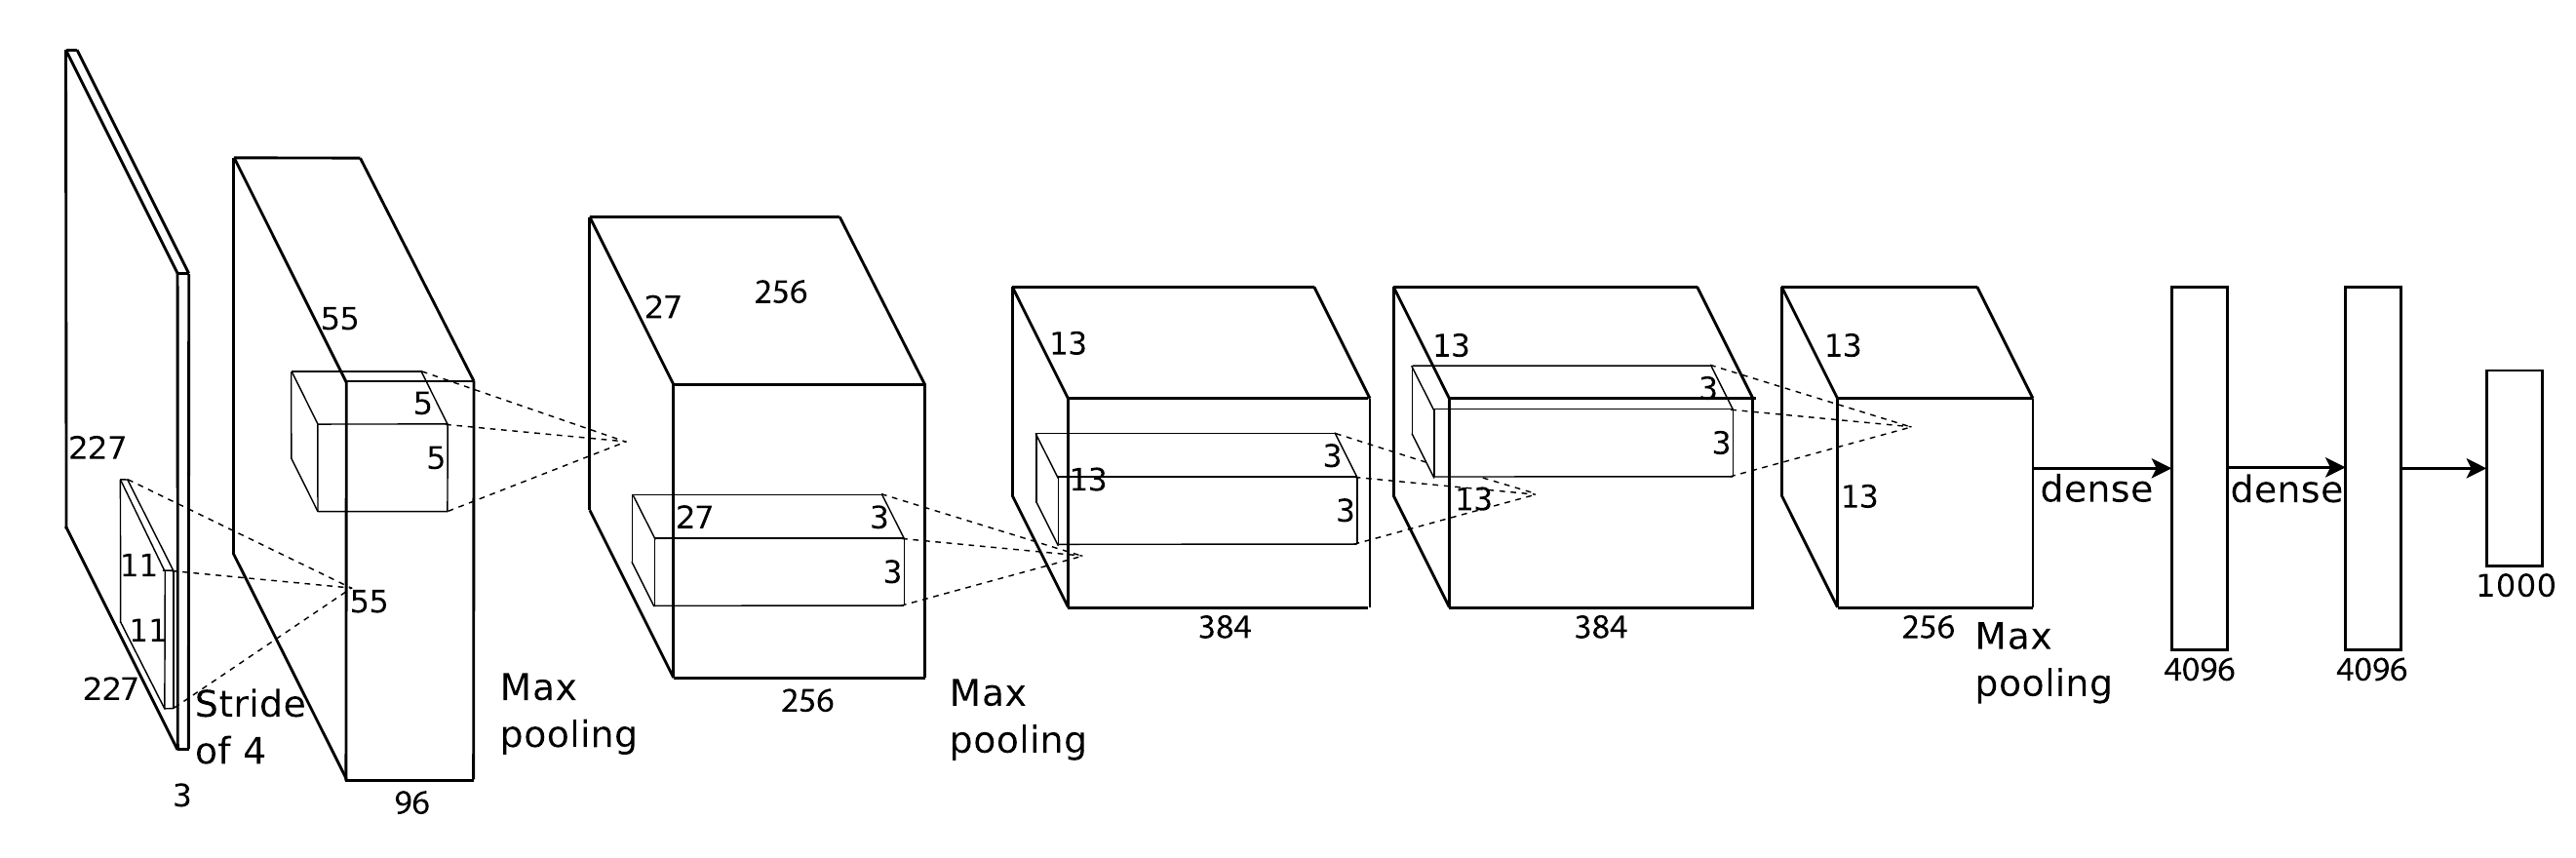
\includegraphics[width=0.95\textwidth]{capitulos/cap_02/imagenes/CNN_complete.png}
    \caption[
        Esquema gráfico de la arquitectura conocida como ``AlexNet'', diseñada para resolver un problema
        de clasificación con 1000 clases.
        Recuperado de la Figura 5.39 de \cite{szeliski2010}.
    ]{
        Esquema gráfico de la arquitectura conocida como ``AlexNet'', diseñada para resolver un problema
        de clasificación con 1000 clases.
        Recuperado de la Figura 5.39 de \cite{szeliski2010}.
        Esta arquitectura presenta una serie de capas convolucionales con funciones de activación no lineales 
        ReLU y max pooling, que formarían el \textit{backbone} y una serie de capas FC (\textit{classifier}), 
        con una capa final softmax, que aplimentad una función de pérdida de entropía cruzada multiclase.
    } 
    \label{fig:CNN_complete}
\end{figure}


\subsubsection{Regularización y normalización}

Como en otras arquitecturas de redes neuronales, existen numerosas técnicas de regularización para evitar
el sobreajuste. Veamos algunas de las técnicas empleadas en CNNs:

\begin{itemize}

    \item \textbf{\textit{Data augmentation}} \cite{chen2019,zhang2021}: Consiste en añadir o modificar 
    dinámicamente ejemplos a partir de los que se tienen originalmente, de forma que se entrene la red con 
    un conjunto de datos más diverso y robusto, evitando el sobreajuste y mejorando la generalización.
    
    Algunas alteraciones realizadas pueden ser cambios en el nivel de brillo y contraste, rotaciones, 
    traslaciones, escalados o volteos de imágenes, entre otras. No existe configuración óptima, y su 
    configuración depende mucho del problema y las imágenes disponibles.

    Esta técnica sirve especialmente para problemas como clasificación o regresión, donde las clases o valores 
    predichos no suelen variar bajo pequeñas perturbaciones locales. 
    
    \item \textbf{\textit{Dropout}} \cite{srivastava2014}: Técnica que, durante el entrenamiento, ``apaga'' 
    (pone a cero) aleatoriamente un porcentaje de neuronas en cada iteración, evitando así que la red 
    dependa demasiado de determinadas unidades individuales (véase la Figura \ref{fig:net_with_dropout}). 
    En CNNs suele aplicarse a capas \textit{fully-connected}, 
    aunque existen variantes como \textit{Spatial Dropout} \cite{tompson2015} que elimina canales completos 
    en capas convolucionales, forzando una distribución más robusta de características.

    \begin{figure}[h]
        \centering

        \begin{subfigure}[b]{0.45\textwidth}
            \centering
            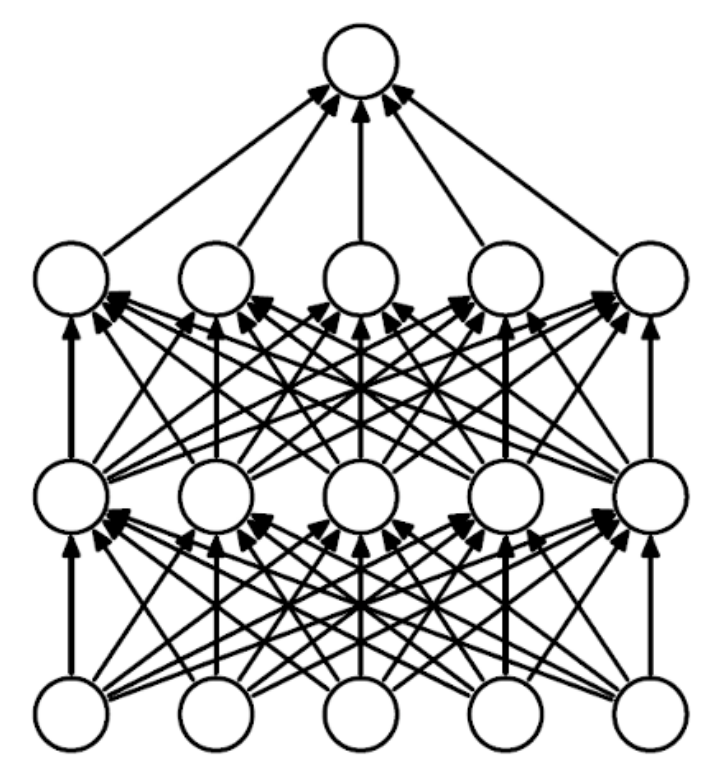
\includegraphics[width=\textwidth]{capitulos/cap_02/imagenes/net_without_dropout.png}
            \caption{Dropout desactivado}
            \label{fig:net_deactivate_dropout}
        \end{subfigure}
        \hfill
        \begin{subfigure}[b]{0.45\textwidth}
            \centering
            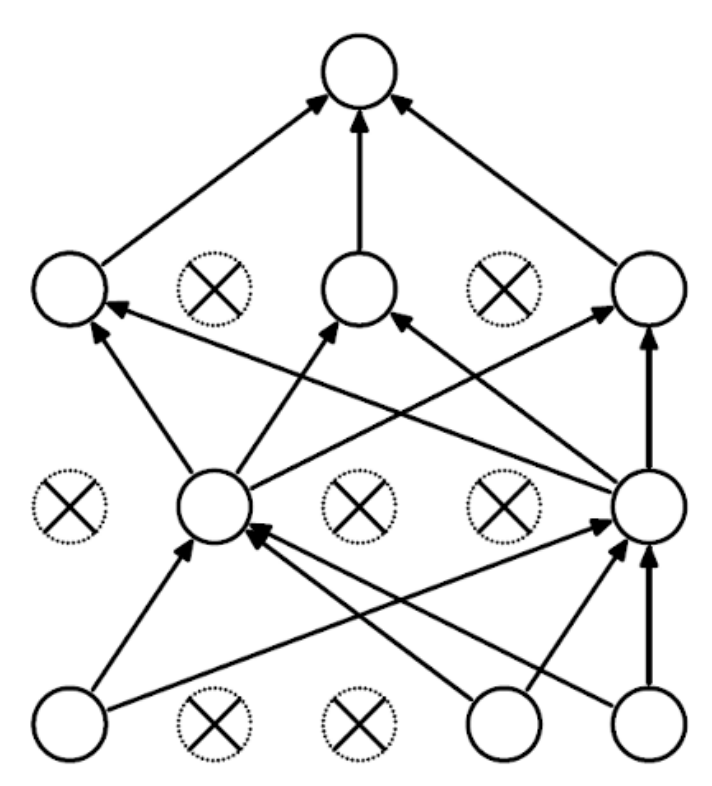
\includegraphics[width=\textwidth]{capitulos/cap_02/imagenes/net_with_dropout.png}
            \caption{Dropout activado ($p=0.5$)}
            \label{fig:net_activate_dropout}
        \end{subfigure}

        \caption[
            Diagrama del funcionamiento de neuronas con \textit{dropout}.
            Recuperado de la Figura 5.29 de \cite{szeliski2010}.
        ]{
            Diagrama del funcionamiento de neuronas con \textit{dropout}.
            Recuperado de la Figura 5.29 de \cite{szeliski2010}.
            Cuando se evalúa el modelo, todas las unidades funcionan correctamente 
            (\ref{sub@fig:net_deactivate_dropout}). Durante el entrenamiento, algunas son ``apagadas'' 
            (\ref{sub@fig:net_activate_dropout}). 
        }
        \label{fig:net_with_dropout}
    \end{figure}
    
    \item \textbf{\textit{Batch normalization}} \cite{ioffe2015}: Esta se introduce como una capa nueva a 
    añadir en el diseño de las redes, con nuevos parámetros entrenables: \textit{scale} y \textit{shift}. 
    Normaliza los valores de cada canal (media cero y desviación 1), y los reescala y desplaza en base a los
    valores de \textit{scale} y \textit{shift}. 
    Esto suaviza significativamente el espacio de valores de optimización \cite{santurkar2019} y reduce la 
    sensibilidad a la tasa de aprendizaje \cite{arora2018}, permitiendo establecer valores más altos.
    En CNNs se aplica típicamente después de las capas convolucionales y antes de la función de activación
    
\end{itemize}


\subsubsection{Conexiones residuales}

Uno de los principales problemas que no permite aumentar mucho la profundidasd de las redes convolucionales 
es el desvanecimiento de gradiente (\textit{vanishing gradient problem}), que consiste en la disminución 
exponencial de los gradientes durante el proceso de \textit{backpropagation} a medida que se retrocede hacia 
las capas iniciales de la red. Algunas de las soluciones a este problema han sido: utilizar funciones de 
activación ReLU, ya que evita gradientes pequeños para valores positivos; inicializar adecuadamente los pesos
de la red; o \textit{batch normalization}, que estabiliza la distribución de las activaciones. Sin embargo,
las conexiones residuales han sido la contribución más significativa para resolver este problema.

Las \textbf{redes residuales (\textit{residual nets}, ResNet)} 

\todo{A completar más tarde}

%https://www.jeremyjordan.me/nn-learning-rate/



% ------------------------------------------------------------------------------------------------------------

\subsection{Transfer Learning}

El \textbf{aprendizaje por transferencia (\textit{transfer learning})} es una técnica que consiste en 
aprovechar el conocimiento aprendido por un modelo entrenado en una tarea como punto de partida para
mejorar el rendimiento y acelerar el entrenamiento en una nueva tarea relacionada \cite{rusell2021}.

En redes neuronales, el aprendizaje consiste en ajustar pesos, y en el caso del \textit{transfer learning}, 
estos pesos se inicializan con valores previamente optimizados para una tarea fuente, en lugar de comenzar con 
valores aleatorios (véase la Figura \ref{fig:fine-tuning}).

Se conoce como \textbf{fine-tuning} a la técnica de inicialización de los pesos de aquellas partes del modelo 
(como capas convolucionales) con los pesos previamente aprendidos, y que continúa el entrenamiento con los 
datos específicos de la nueva tarea. En este contexto, se denomina \textit{head} a las capas finales del 
modelo que se sustituyen para adaptarse a la nueva tarea. 

\begin{figure}[h]
    \centering
    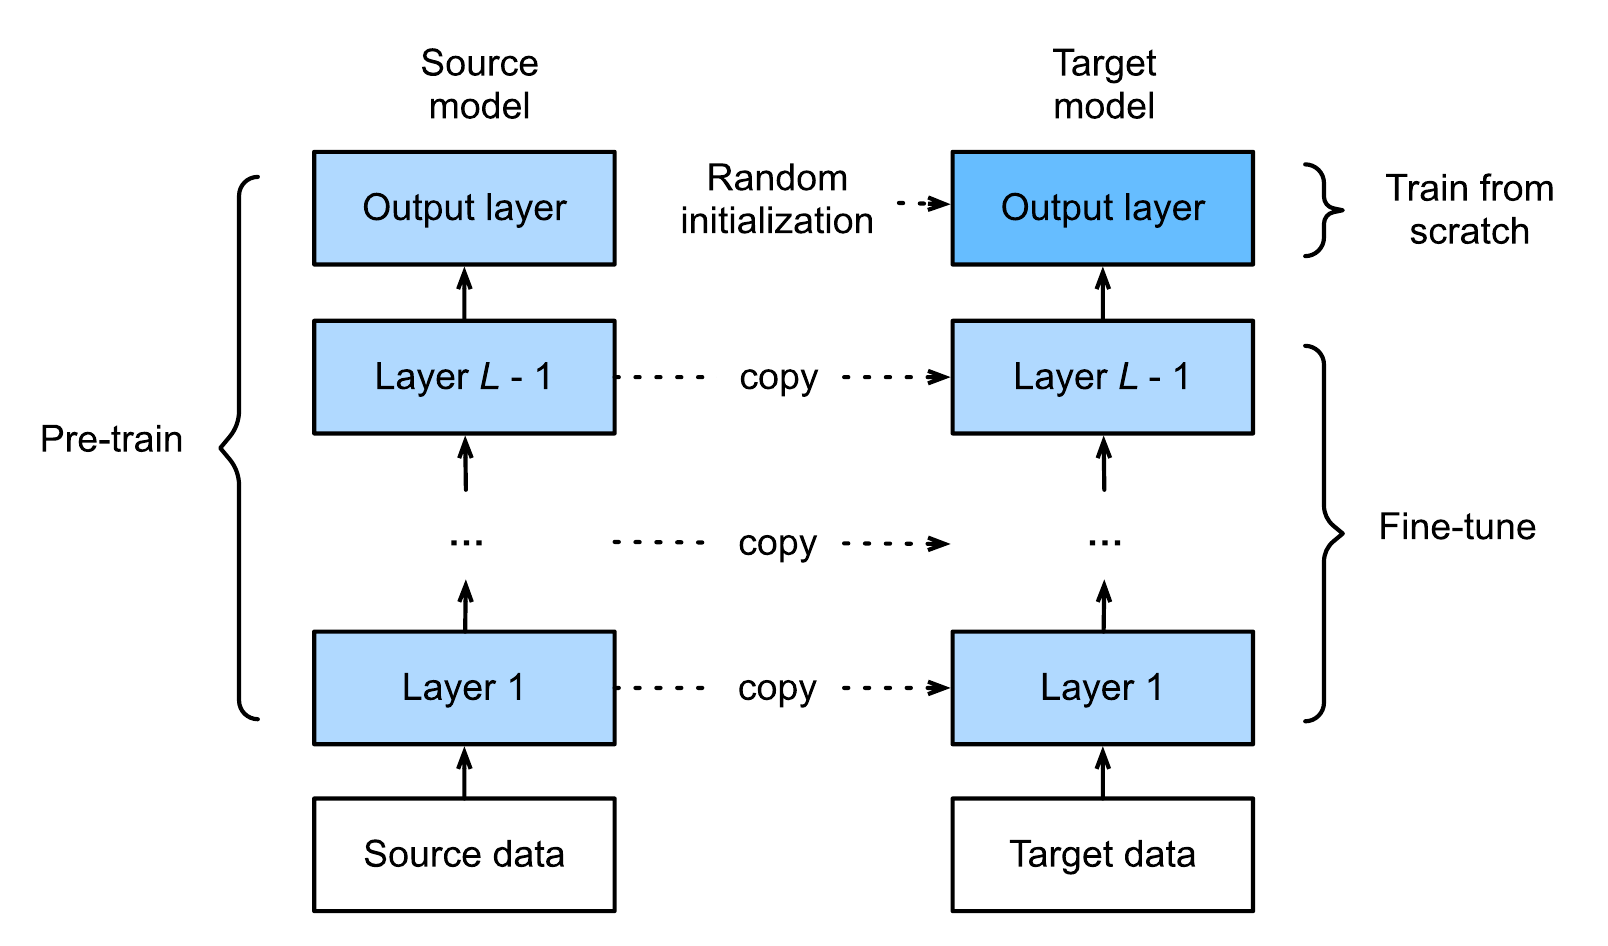
\includegraphics[width=0.95\textwidth]{capitulos/cap_02/imagenes/fine-tunning.png}
    \caption[
        Diagrama de \textit{fine-tuning} de un modelo en una nueva tarea. 
        Recuperado de la Figura 19.2 de \cite{murphy2022}.
    ]{
        Diagrama de \textit{fine-tuning} de un modelo en una nueva tarea. 
        Recuperado de la Figura 19.2 de \cite{murphy2022}.
        La capa final de salida es entrenada desde cero para la nueva tarea. El resto de capas son 
        inicializadas con los pesos previos. 
    } 
    \label{fig:fine-tuning}
\end{figure}

Por ejemplo, en \cite{venema2022} se utilizan dos modelos de CNN preentrenados en clasificación con ImageNet 
(que contiene imágenes de 1000 clases): VGG16 y ResNet50. Estos modelos se ajustan (\textit{fine-tuning}) 
para estimar el sexo de una persona a partir de radiografías de húmero. Aunque ambas tareas parecen muy 
diferentes, las primeras capas de la red, especializadas en detectar características generales como bordes y 
texturas, pueden ser útiles en los dos casos, lo que permite una transferencia efectiva del conocimiento.

El \textit{fine-tuning} puede aplicarse de forma gradual: primero se entrena solo el \textit{head} 
(manteniendo el resto del modelo congelado) y luego, si es necesario, se afinan también algunas capas 
preentrenadas para mejorar el rendimiento en la tarea específica.


% ------------------------------------------------------------------------------------------------------------
% INCERTIDUMBRE ----------------------------------------------------------------------------------------------
% ------------------------------------------------------------------------------------------------------------

\section{Incertidumbre}

La metrología
\footnote{
    Ciencia de las mediciones y sus aplicaciones \cite{jcgm200:2012}.
},
y la estadística comparten un papel fundamental en el análisis del error y la incertidumbre en campos como 
el ML. Mientras la metrología establece los fundamentos conceptuales de error e incertidumbre, la estadística 
proporciona métodos para cuantificar, modelar y reducir estos factores durante el desarrollo y validación de 
modelos.

El Comité Conjunto de Guías en Metrología (\textit{Joint Committe for Guides in Metrology})
\footnote{
    Este Comité está formado por numerosas organizaciones internacionales de metrología y normalización: 
    BIPM, IEC, IFCC, ISO, IUPAC, IUPAP, OIML e ILAC. Su objetivo principal es mantener y promover las 
    guías internacionales clave en metrología, como la Guía para la Expresión de la Incertidumbre en la 
    Medición (\textit{Guide to the Expression of Uncertainty in Measurement}) \cite{jcgm100:2008} y el 
    Vocabulario Internacional de Metrología (\textit{Vocabulaire international de métrologie}) 
    \cite{jcgm200:2012}.
}
define el \textbf{error} como una ``medición imperfecta'' de la magnitud observada, que puede estar causada
por efectos aleatorios (componente aleatoria del error) y por efectos sistemáticos (componente sistemática del 
error, más conocida como \textbf{sesgo}).
Por otro lado, define a la \textbf{incertidumbre} como ``parámetro, asociado con el resultado de una medición, 
que caracteriza la dispersión de los valores que podrían atribuirse razonablemente al \textbf{mensurado}, que
es como se denomina a la magnitud a ser medida. [...] El parámetro puede ser, por ejemplo, una desviación 
estándar, o la anchura de un intervalo con un nivel de confianza establecido'' \cite{jcgm100:2008}.

Partiendo de estas definiciones generales, veamos las diferencias entre los dos enfoques principales en la 
evaluación de mediciones: el enfoque basado en el error y el enfoque basado en la incertidumbre.

El \textbf{enfoque basado en el error} o enfoque tradicional parte de la premisa de que existe un valor 
verdadero. En consecuencia, el propósito de la medición es aproximarse lo más posible a dicho valor, 
minimizando las distintas componentes del error \cite{jcgm100:2008}:

\begin{itemize}

    \item para el error aleatorio, esto se logra aumentando el número de observaciones, ya que su distribución 
    tiende una media igual a cero; y

    \item para el error sistemático, es necesario identificarlo y cuantificar su magnitud, lo que permite 
    aplicar factores de corrección que compensen su efecto.

\end{itemize}

Se asume que el resultado de la medición ha sido corregido por todos los efectos sistemáticos identificados
como significativos, de modo que la esperanza matemática de esta componente sea igual a cero.

Sin embargo, en la práctica no existen reglas claras para distinguir las componentes del error ni cómo estas 
se combinan en el error total. En general, solo es posible estimar un límite superior del valor 
absoluto del error total estimado, al que se denomina de forma inapropiada ``incertidumbre''. 

Frente al enfoque anterior, se presenta el \textbf{enfoque basado en la incertidumbre} \cite{jcgm100:2008}, 
cuyo propósito no es hallar el mejor valor posible, sino establecer un intervalo de valores razonables para el 
mensurando, el cual puede refinarse con información adicional. Así, la medición misma se convierte en una 
herramienta para determinar el error potencial del instrumento ---o modelo en ML---. 

% ------------------------------------------------------------------------------------------------------------

\subsection{Incertidumbre en \textit{machine learning}}

Las fuentes de incertidumbre pueden ser muy variadas, y su identificación requiere en muchos casos de 
conocimiento específico en el problema, si bien se suelen considerar dos tipos de incertidumbre en las 
predicciones realizadas en ML \cite{hullermeier2021, nemani2023}:

\begin{itemize}
    
    \item La \textbf{incertidumbre aleatoria o estocástica} procede de la variabilidad aleatoria de un 
    fenómeno. 
    Es irreducible por naturaleza, aunque se disponga de más datos. 
    Un ejemplo típico es el resultado de lanzar una moneda al aire. Incluso el mejor modelo solo será capaz de 
    dar probabilidades para las dos posibles salidas, sin una respuesta definitiva. 
    
    % En ML, esta incertidumbre representa la naturaleza inherentemente estocástica de las entradas, las salidas 
    % y la dependencia entres estas dos. 

    En el contexto de la estimación de la edad forense, esta incertidumbre se manifiesta en las diferentes 
    edades biológicas que puede estimarse a individuos de la misma edad cronológica.
    Se sabe que existe una correlación entre edad biológica y la cronológica, pero esta no es perfecta, 
    debido a que existe variabilidad inherente al problema.

    % \begin{itemize}
    %     \item las entradas. Por ejemplo, 
        
    %     \item las salidas. Por ejemplo, el resultado de lanzar una moneda al aire; incluso el mejor modelo 
    %     solo será capaz de dar probabilidades para las dos posibles salidas, sin una respuesta definitiva.
        
    %     \item la dependencia entre las anteriores. Por ejemplo, estimar la edad cronológica de un esqueleto  
    %     un esqueleto de determina edad biológica
    
    % \end{itemize}


    \item La \textbf{incertidumbre epistémica} es la causada por falta de conocimiento o precisión del modelo.
    Se relaciona con aspectos como la escasez de datos, la calidad de la información disponible, las 
    limitaciones teóricas y prácticas del modelo escogido, etc. 
    A diferencia de la incertidumbre aleatoria, esta sí es reducible por naturaleza; puede reducirse con más
    datos, mejores modelos o mayor comprensión del problema. 
    
\end{itemize}

A estos, se le puede añadir un tercer tipo: el \textbf{\textit{drift}} \cite{gama2012, nemani2023}, que 
procede de cambios en la distribución de los datos a lo largo del tiempo, ya sea en la distribución de las 
variables de entrada, en la distribución de las variables de salida, o en la relación entre las dos previas. 
Por ejemplo: una imagen de entrada a un modelo de clasificación que no corresponde a ninguna clase con la que 
se haya entrenado anteriormente; un cambio en la población objetivo de una aplicación médica ---p.ej., debido 
a un cambio demográfico o a la aparición de una nueva enfermedad---; o la toma de imágenes médicas con una 
máquina distinta a la que se empleó para obtener las imágenes con las que se ha entrenado el modelo.

% ------------------------------------------------------------------------------------------------------------

\subsection{Cuantificación de la incertidumbre en \textit{machine learning}} 

El desarrollo de las técnicas modernas de ML ha estado principalmente centrado en la minimización y 
cuantificación del error de predicción. Este enfoque ha permitido que el aprendizaje automático despliegue un 
gran potencial en multitud de aplicaciones.
Sin embargo, cuando se trata de aplicaciones críticas ---como la medicina, los sistemas financieros o el 
control de infraestructuras--- surge una necesidad esencial: no solo importa cuán precisa es una predicción, 
sino también cuán confiable es \cite{begoli2019}. 
En respuesta a esta necesidad, durante la última década se ha producido un creciente interés y desarrollo de 
técnicas orientadas a la explicabilidad e interpretabilidad de la IA 
\cite{angelov2021, ali2023, miller2019, loh2022} y la cuantificación de la incertidumbre
\cite{abdar2021, psaros2023, nemani2023}.

Mientras la explicabilidad de la IA busca entender las razones detrás de cada predicción centrándose en el 
estudio del modelo y arquitectura concretos \cite{salvi2025}, la 
\textbf{cuantificación de la incertidumbre (\textit{uncertainty quantification}, UQ)} evalúa el grado de 
confianza en las predicciones realizadas y se centra en caracterizar las fuentes de variabilidad y posible 
error en los datos, el modelo y el entorno de aplicación \cite{nemani2023}.

Existe una gran variedad de técnicas de UQ. Estas técnicas pueden clasificarse de distintas formas: algunas 
son \textit{model-agnostic}, es decir, pueden aplicarse a cualquier tipo de modelo sin 
requerir acceso a su estructura interna; otras son \textit{model-specific}, diseñadas para aprovechar 
características particulares del modelo subyacente. 
Algunas técnicas suponen que los datos siguen ciertas 
distribuciones estadísticas explícitas, mientras que otras operan sin realizar tales suposiciones. 
También existen métodos que asumen intercambiabilidad entre observaciones, frente a aquellos que no lo hacen 
y requieren estructuras de dependencia más complejas. 

Los métodos más populares son \textit{gaussian process regression} (GPR),

redes neuronales bayesianas (\textit{bayesian neural networks}, BNNs),
redes neuronales \textit{ensemble}, 
métodos deterministas

\begin{itemize}
    \item \textbf{Procesos de regresión gausiana (\textit{gaussian process regression}, GPR)}: 
    
    \item \textbf{Técnicas bayesianas}: Estas emplean

    \item \textbf{Técnicas \textit{ensemble}}:  
\end{itemize}




% ¿Qué es la cuantificación de incertidumbre?

% Es un proceso añadido sobre el actual proceso de entrenamiento de un modelo, ya sea ..., 
% que genera un intervalo o distribución 




% La UQ puede abordarse desde dos perspectivas diferentes: 

% \begin{itemize}

%     \item sobre datos ya observados (como los de entrenamiento o validación), donde el objetivo es evaluar si 
%     el modelo representa adecuadamente la variabilidad de los datos, detectar sobreajuste o validar la 
%     calibración de las predicciones; o
    
%     \item sobre nuevos datos (no vistos), donde el objetivo es estimar la confianza del modelo en situaciones 
%     reales de predicción, donde no se conoce el valor verdadero.

% \end{itemize}

% Algunos métodos de cuantificación de la incertidumbre

% % Hablar sobre métodos de UQ en datos ya observados

% Nos centraremos en el estudio de la cuantificación de la incertidumbre sobre datos nuevos, pues es en este 
% contexto donde resulta más relevante para aplicaciones prácticas, como las de estimación del PB. 
% Esta provee información clave para la toma de decisiones tanto del valor predicho como de la certeza asociada
% a la predicción. 
% \todo{
%     ¿Es posible hablar de métodos de cuantificación de incertidumbre sobre datos nuevos sin mencionar los
%     métodos sobre datos previos? En clasificación, la calibración del modelo es importante para la 
%     cuantificación de incertidumbre. De hecho, es recomendable realizarla previamente a la aplicación de 
%     conformal prediction.
% }

% En problemas de regresión, es deseable que los modelos no solo proporcionen una 
% predicción puntual, sino también un intervalo que indique el grado de incertidumbre asociado a cada 
% predicción, conocido como \textbf{intervalo de predicción (\textit{prediction interval})},
% el cual puede derivarse de métodos de UQ como %%%%%%AÑADIRR MÁS \textit{bootstrapping} o predicción conformal

% Además, nos centraremos en aquellos métodos que no requieran asumir distribuciones específicas en los datos
% ni dependan fuertemente de supuestos paramétricos, ya que en muchos problemas reales (como la 
% estimación del perfil biológico) los datos pueden presentar heterocedasticidad, asimetría o 
% comportamientos complejos que dificultan su modelización con enfoques clásicos.





% \subsubsection{Cuantificación de la incertidumbre en problemas de regresión}

% Existe multitud de maneras de cuantificar la incertidumbre en problemas de regresión.

% % Comenzar hablando sobre los intervalos de predicción

% % Reestructurar

% Una primera aproximación es la \textbf{regresión cuantílica (\textit{quantile regression})}, que añade dos 
% nuevas salidas en el modelo de regresión, que serán los límites inferior y superior de un intervalo de 
% predicción, correspondientes a cuantiles específicos (por ejemplo, los percentiles 10 y 90)
% \footnote{
%     El entrenamiento del modelo para estas dos salidas se realiza con la función de pérdida \textit{pinball},
%     \cite{steinwart2011} que combina los errores de predicción para múltiples cuantiles, penalizando
%     asimétricamente las desviaciones según el cuantil objetivo.
% }. 
% Esto permite estimar no solo la tendencia central (como en la regresión tradicional), sino también la 
% incertidumbre de las predicciones (véase la Figura \ref{fig:quantile_regression}).

% \begin{figure}[h]
%     \centering
%     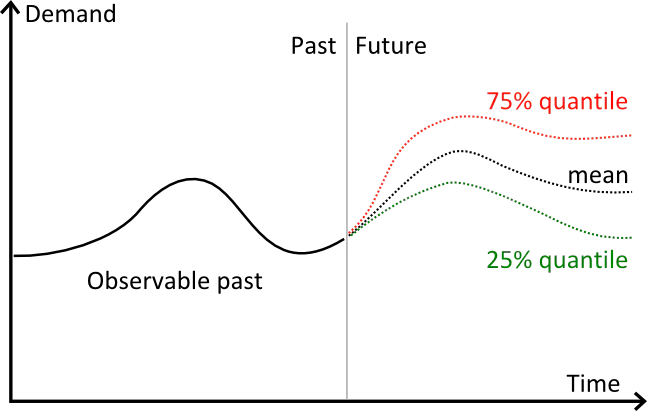
\includegraphics[width=0.8\textwidth]{capitulos/cap_02/imagenes/quantile_regression.png}
%     \caption[
%         Gráfico que ilustra las 3 predicciones que arroja un modelo de regresión cuantílica. Recuperado de 
%         \cite{vermorel2012}.
%     ]{
%         Gráfico que ilustra las 3 predicciones que arroja un modelo de regresión cuantílica. Recuperado de 
%         \cite{vermorel2012}. Se observa los límites superior e inferior los percentiles 75 y 25, 
%         respectivamente. 
%     }
%     \label{fig:quantile_regression}
% \end{figure}

% Sin embargo, este método presenta varios problemas:

% \begin{itemize}

%     \item Sensibilidad a datos escasos o ruidosos: La estimación puede ser muy sensible a 
%     \textit{outliers}
%     \footnote{
%         Los valores atípicos o \textit{outliers} son instancias que se desvían significativamente del resto
%         de instancias del conjunto de datos. Un \textit{outlier} podría indicar un comportamiento anormal
%         del sistema (variabilidad natural del fenómeno observado, eventos excepcionales que refleja 
%         comportamientos reales pero poco frecuentes, ...) o un error de recolección y registro de los datos 
%         \cite{alpaydin2010}.   
%     } 
%     y a regiones con pocas observaciones, llevando a intervalos poco fiables. De hecho, se puede dar el 
%     fenómeno indeseable de que cuantiles mayores tengan valores predichos más bajos que cuantiles menores 
%     ---conocido como cruzamiento de cuantiles \cite{koenker2005}---.
    
%     \item Falta de cobertura probabilística garantizada: No existe ningún tipo de garantía estadística que 
%     asegure que el cuantil estimado cubra la proporción deseada de observaciones en muestras futuras. 
    
%     \item No captura la incertidumbre epistémica: Solo captura la incertidumbre aleatoria \cite{abdar2021},
%     dado que modela cómo los valores de salida varían dado un conjunto de entradas. No captura automáticamente 
%     incertidumbre epistémica, a menos que se combine con otros enfoques, como métodos bayesianos 
%     \cite{tokdar2012}.

%     \item Muestran gran incertidumbre en cuantiles extremos (cerca de cero o uno) \cite{feldman2023} y, por 
%     tanto, los intervalos de predicción obtenidos son extremedamente grandes, lo que logra una gran cobertura
%     pero poca utilidad práctica. 
    
% \end{itemize}


% Otra técnica que no ...


% \todo{Introducir la predicción conformal}



% \subsubsection{Cuantificación de la incertidumbre en problemas de clasificación}

% Por otro lado, en el caso de los problemas de clasificación, el concepto equivalente
% al de intervalo de predicción se denomina \textbf{conjunto de predicción (\textit{prediction set})}, 
% que puede construirse mediante técnicas como estimaciones de probabilidad calibrada o predicción conformal. 



% \todo{¿Introducir la calibración de modelos y centrarse en el Platt Scaling y Temperature Scaling?}


% \todo{Introducir la predicción conformal}



% ------------------------------------------------------------------------------------------------------------
% CONFORMAL PREDICTION ---------------------------------------------------------------------------------------
% ------------------------------------------------------------------------------------------------------------

\section{Predicción conformal}

La \textbf{predicción conformal (\textit{conformal predition}, CP)} \cite{vovk2005} es un marco teórico para 
la UQ en modelos de ML, que proporciona intervalos o conjuntos de predicción con garantías estadísticas de 
cobertura. Estas garantías son válidas bajo el supuesto mínimo de intercambiabilidad de los datos, sin 
requerir hipótesis sobre la distribución subyacente de los mismos.
Sin embargo, esta robustez tiene un coste: la CP requiere un conjunto de datos adicional para 
\textbf{calibración}, que es el proceso por el cual se ajustan los intervalos de predicción para garantizar 
las propiedades estadísticas prometidas.
Vamos a definir más en detalle estos puntos.

% ------------------------------------------------------------------------------------------------------------

\subsection{Propiedades de la predicción conformal}

La CP garantiza que las predicciones contengan el valor verdadero con al menor una probabilidad $1-\alpha$, 
donde $\alpha$ es el nivel de significación:

$$
P(Y_{n+1} \in \hat{C_\alpha}(X_{n+1})) \ge 1 - \alpha
$$

Esta propiedad se denomina \textbf{cobertura marginal válida} \cite{prinster2024}, y se cumple para todas las 
entrada $X$, siempre y cuando los datos sean intercambiables (\textit{interexchangeable}), es decir, todos los 
datos procedan de la misma distribución y, por tanto, la posición del nuevo ejemplo dentro del conjunto 
completo de datos sea estadísticamente indistinguible del resto. Esta intercambiabilidad en imágenes 
implicaría que todas fueran tomadas en condiciones más o menos similares: mismo dominio, distribución de 
valores de salida, iluminación, resolución, estilo, etc.

En cambio, la CP no asegura \textbf{cobertura condicional válida} \cite{foygel2021}; es decir, no es posible 
garantizar cobertura para todos los subgrupos de datos sin hacer suposiciones fuertes o sacrificar utilidad 
práctica, en concordancia con el conocido Teorema \textit{No Free Lunch} \cite{wolpert1997}. 
Además, el conjunto de calibración debe ser estadísticamente representativo de la distribución completa de los 
datos. Esto crea un compromiso fundamental: asignar más muestras a la calibración mejora la precisión de los 
intervalos predictivos, pero a costa de reducir el tamaño del conjunto de entrenamiento, lo que potencialmente 
puede empeorar el rendimiento del modelo base.

Bajo estas garantías estadísticas, el verdadero potencial de la CP está en su flexibilidad para ser 
integradas con otros métodos UQ.

Algunas características deseables en las técnicas de CP son:

\begin{itemize}
    \item \textbf{Independencia del modelo (\textit{model-agnostic})}: que no requiera reentrenar el modelo ni 
    modificar su arquitectura, permitiendo su aplicación \textit{post-hoc} a modelos preentrenados.

    \item \textbf{Independencia del dominio (\textit{domain-agnostic})}: que pueda manejar entradas de 
    cualquier tipo sin restricciones. 
     
    \item \textbf{Predicción adaptativa (\textit{adaptive prediction})}: que se muestre mayor incertidumbre 
    ---y por tanto, máyo rango o conjunto de valores--- en las predicciones a más ``difíciles''
    \footnote{
        La dificultad es un criterio a priori subjetivo que hay que definir objetivamente ---o, en su defecto,
        dejar que un modelo lo aprenda en base a otros parámetros objetivos---.
    } sean estas. 

    \item \textbf{Ser eficiente computacionalmente}: es preferible que tanto la calibración como la inferencia 
    no sean computacionalmente muy costosas. 
    
    \item \textbf{Robustez frente a datos ruidosos y detección de datos \textit{out-of-distribution}}
    \footnote{
        Los datos \textit{out-of-distribution} son datos que no provienen de la misma distribución que los 
        datos con los que se entrenó el modelo.
    }:
    que los intervalos reflejen adecuadamente la incertidumbre ante datos corruptos o fuera del dominio de 
    entrenamiento.  

\end{itemize}

En general, existe un \textit{trade-off} entre flexibilidad y precisión: las técnicas dependientes del modelo,
del dominio o incluso del propio problema (incluyendo información experta), que asumen ciertas distribuciones 
de los datos, cuantifican mejor la incertidumbre aleatoria y epistémica, y suelen producir intervalos más 
ajustados e informativos. 

% ------------------------------------------------------------------------------------------------------------

\subsection{Calibración e inferencia conformal}

La CP en general requiere: introducir un nuevo paso de calibración, en el que se ajusten
las puntuaciones de no conformidad para garantizar validez distribucional; 
y modificar la inferencia para introducir información conformal y realizar la predicción inteválica o conjunto
de predicción.

% ------------------------------------------------------------------------------------------------------------

\subsubsection{Predicción conformal en problemas de regresión}

En los problemas de regresión tendremos, además de la predicción puntual común, dos límites ---inferior y 
superior--- que formarán el intervalo de predicción. 
Este intervalo puede ser simétrico respecto a la predicción puntual o no, dependiendo de la técnica empleada.
En problemas donde se da heterocedasticidad, es decir, cuando la variabilidad del error cambia con respecto a 
los valores de entrada, es especialmente importante utilizar métodos que permitan construir intervalos 
asimétricos.

% Proceso de calibración: ...

El proceso de calibración del modelo consta de los siguientes pasos:

\begin{enumerate}
    \item Se usa el modelo predictivo para realizar las estimaciones puntuales ---o interválicas en caso de la
    regresión cuantílica--- sobre el conjunto de instancias de calibración. 

    
    \item Se calcula una \textbf{puntuación de no conformidad (\textit{nonconformity score})} sobre cada 
    instancia del conjunto de calibración. 
    Esta puntuación de no conformidad debe medir la incertidumbre alrededor de cada predicción. No hay
    restricciones sobre cómo se debe cuantificar esta, salvo que debe presentar la misma distribución de 
    valores en el conjunto de calibración y en los futuros ejemplos, para asegurar la cobertura marginal. 
    Por tanto, puede emplearse tanto entradas, como salidas, representaciones internas del modelo y valores
    reales para arrojar una medida de incertidumbre
    \footnote{
        Cabe decir que una técnica será independiente del modelo y del dominio cuando solo tenga en cuenta
        las salidas del modelo y los valores reales del problema para realizar la CP.
    }.  

    La función de no conformidad más simple para la regresión es el error absoluto.
    Sin embargo, para obtener intervalos asimétricos, se calcula la diferencia entre el valor predicho y el
    real, o viceversa ---dependiendo de si el límite es inferior o superior---. 


    \item Se calcula el cuantil que determina el \textbf{umbral de no conformidad} a utilizar.
    Específicamente, para un nivel de significancia $\alpha$, se selecciona el $(1 - \alpha)(1 + 1/n)$-ésimo 
    cuantil de las puntuaciones de no conformidad obtenidas en el conjunto de calibración, donde $n$ es el 
    número de ejemplos de calibración
    (véase la Figura \ref{fig:nonconformity_quantile_threshold_simetric}). 
    Este valor sirve como corrección para asegurar validez estadística finito-muestral.

    En caso de intervalos asimétricos, se calculan dos umbrales de conformidad (uno por cada cola de la 
    distribución de error), por lo que se selecciona el $(1 - \alpha/2)(1 + 1/n)$-ésimo cuantil de las 
    puntuaciones de no conformidad obtenidas para cada límite 
    (véase la Figura \ref{fig:nonconformity_quantile_threshold_asimetric}).

    \begin{figure}[h]
        \centering

        \begin{subfigure}[b]{0.45\textwidth}
            \centering
            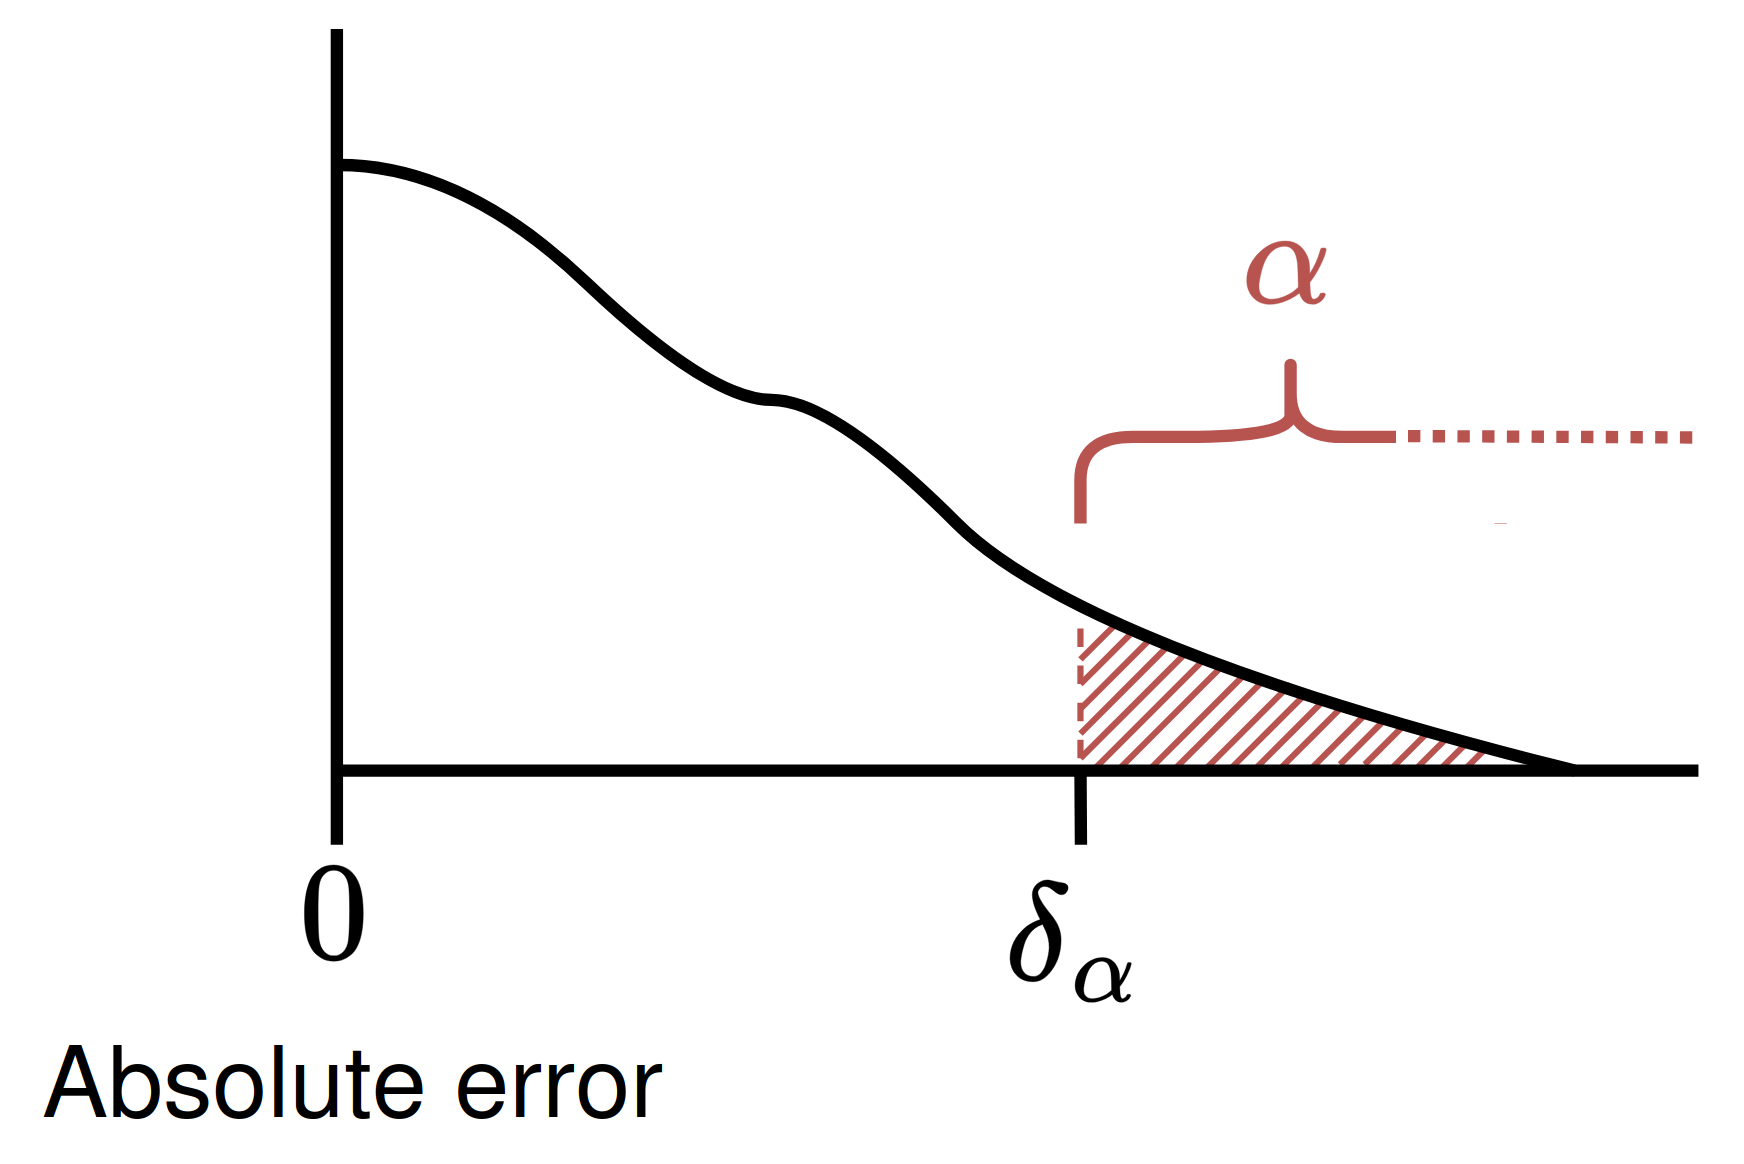
\includegraphics[width=\textwidth]{capitulos/cap_02/imagenes/nonconformity_quantile_threshold_simetric.png}
            \caption{Determinación del umbral de no conformidad para intervalos simétricos.}
            \label{fig:nonconformity_quantile_threshold_simetric}
        \end{subfigure}
        \hfill
        \begin{subfigure}[b]{0.5\textwidth}
            \centering
            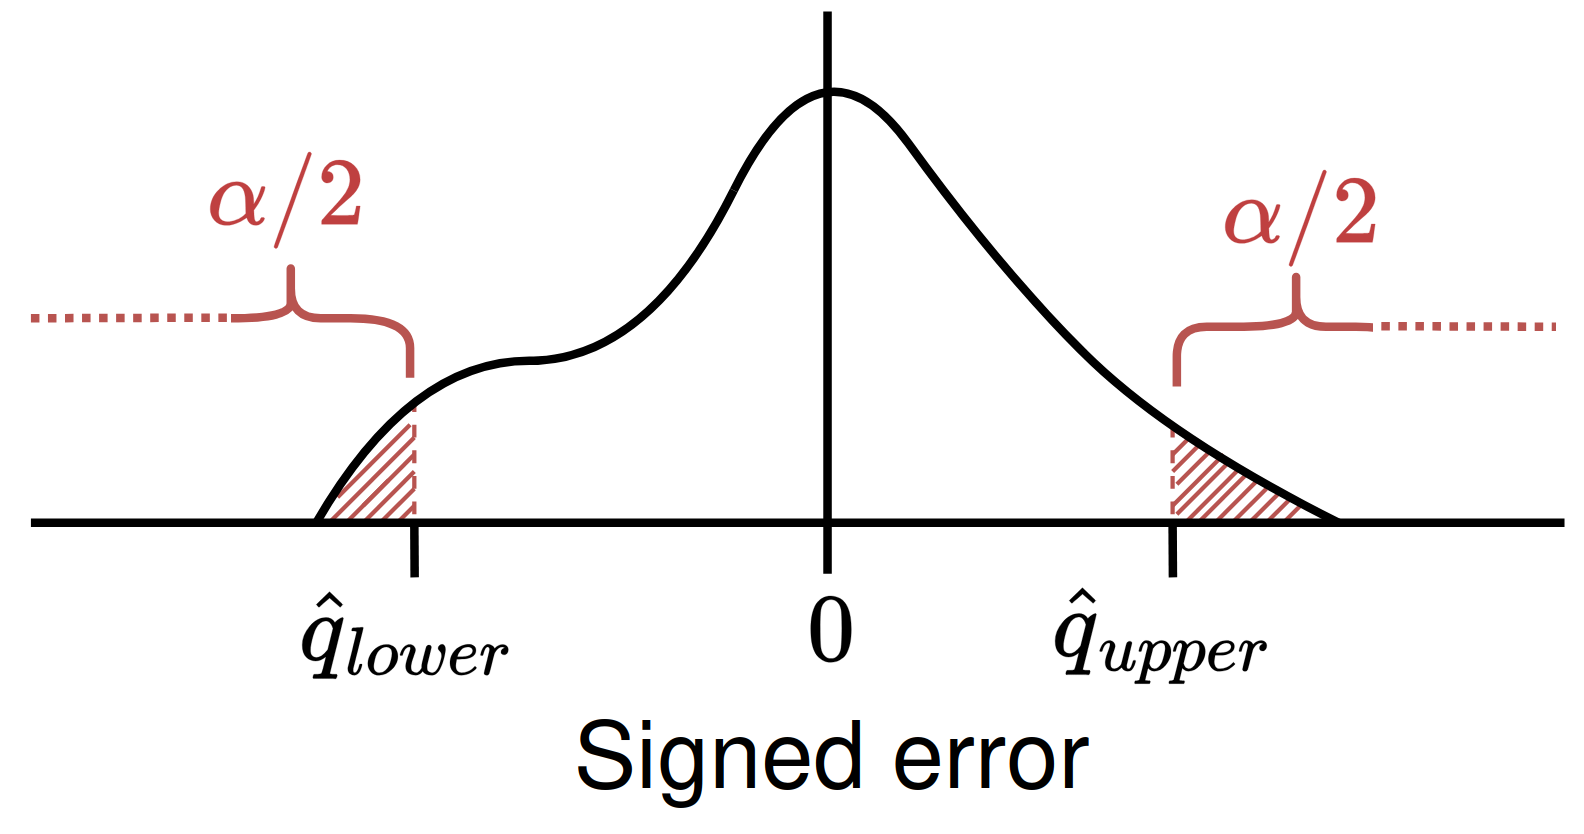
\includegraphics[width=\textwidth]{capitulos/cap_02/imagenes/nonconformity_quantile_threshold_asimetric.png}
            \caption{Determinación de los umbrales de no conformidad para intervalos asimétricos.}
            \label{fig:nonconformity_quantile_threshold_asimetric}
        \end{subfigure}

        \caption[
            Determinación del umbral de no conformidad para intervalos simétricos y asimétricos.
        ]{
            Determinación del umbral de no conformidad para intervalos simétricos y asimétricos. 
            Elaboración propia.
        }
        \label{fig:nonconformity_quantile_comparation}
    \end{figure}

\end{enumerate}

Una vez se ha realizado la calibración, faltaría realizar la inferencia conformal. Para cada predicción de una
nueva instancia:

\begin{enumerate}

    \item Se usa el modelo predictivo para realizar la estimación puntual ---o interválica en caso de la 
    regresión cuantílica--- de la nueva instancia. 
    
    \item Se construye un intervalo predictivo utilizando el valor/es estimado/s y sumando el umbral/es de no
    conformidad. Por ejemplo, para una regresión puntual con intervalo asimétrico, el intervalo conformal 
    sería (sin suponer elementos de escala):

    $$
    \left[ \hat{y_i} + \hat{q}_{lower}, \hat{y_i} + \hat{q}_{upper} \right]
    $$

\end{enumerate}



% ------------------------------------------------------------------------------------------------------------

\subsubsection{Predicción conformal en problemas de clasificación}

\todo{A completar más tarde}




\begin{figure}[h]
    \centering
    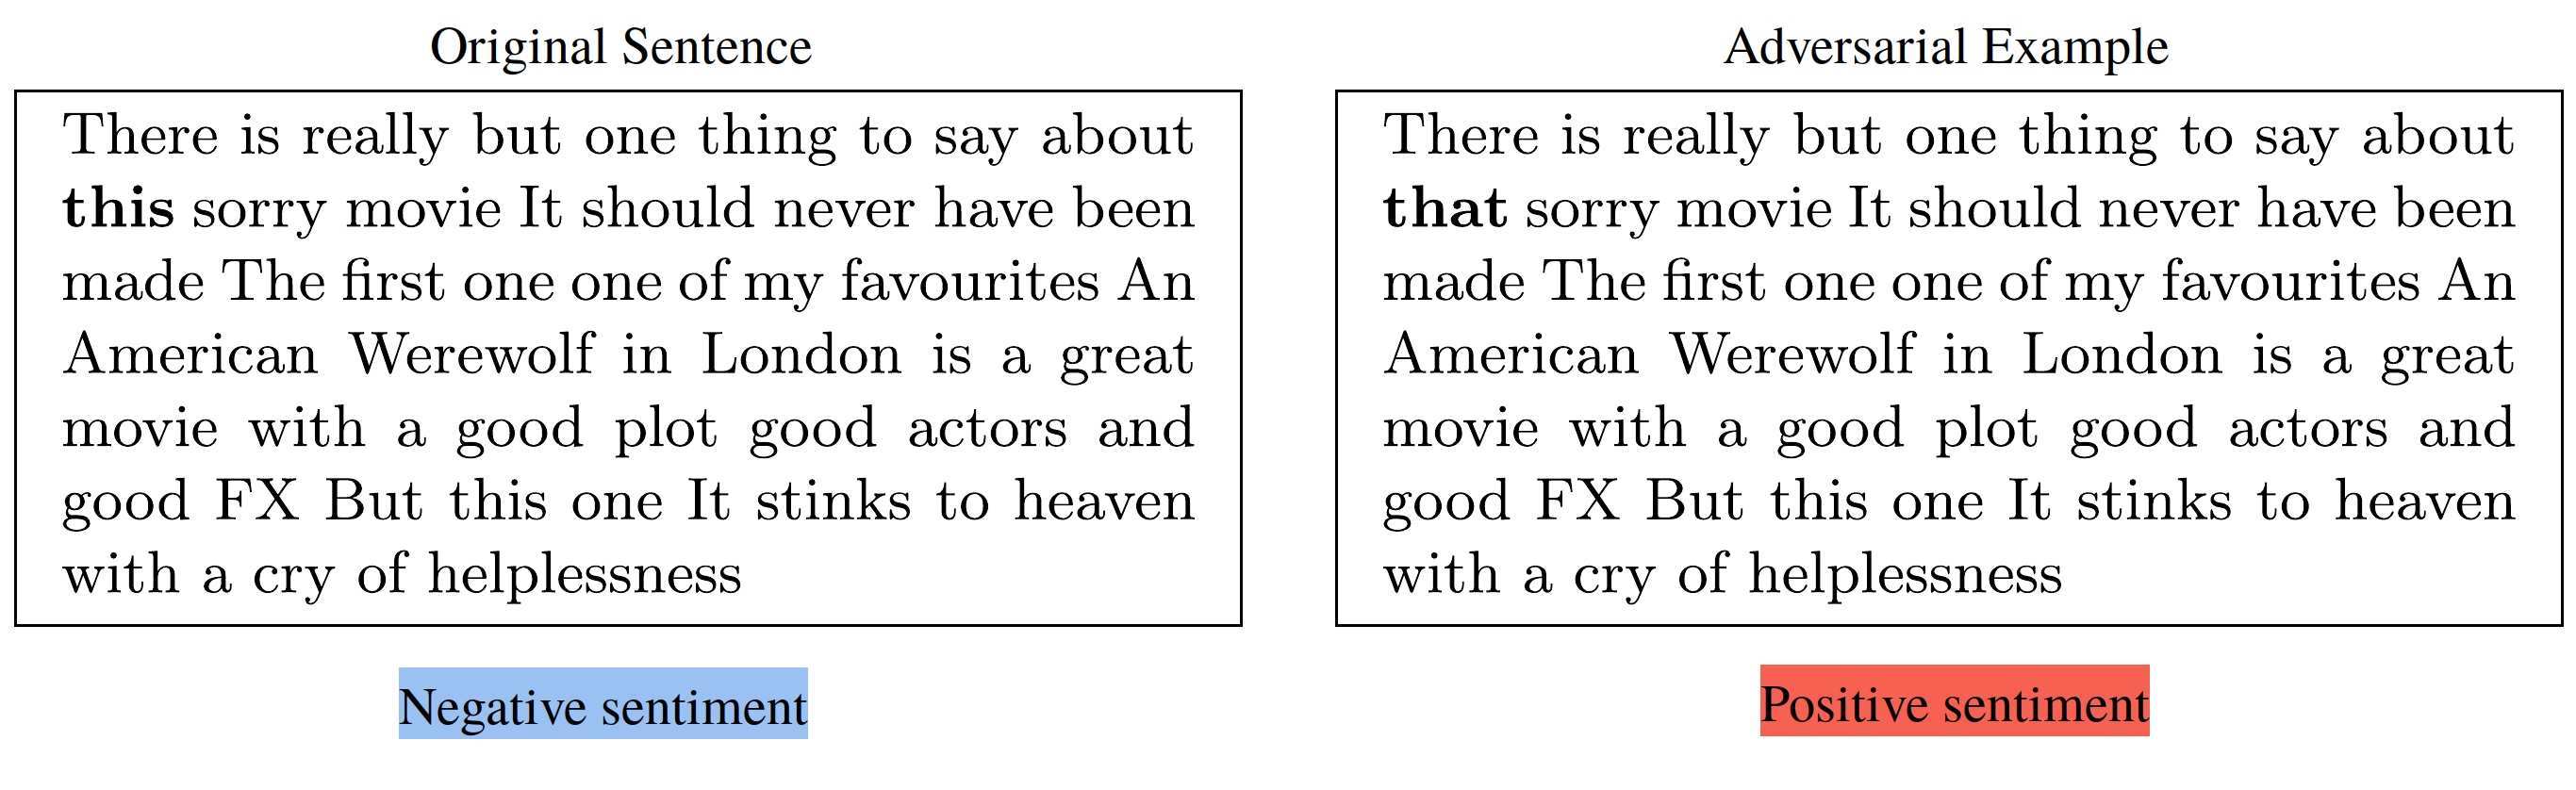
\includegraphics[width=\textwidth]{capitulos/cap_02/imagenes/adversarial_example.png}
    \caption[
        Ejemplo adverario mal clasificado por un modelo ML entrenado con datos textuales.
        Adaptado de la Figura 2 de \cite{hullermeier2021}, original de \cite{sato2018}.
    ]{
        Ejemplo adverario mal clasificado por un modelo ML entrenado con datos textuales.
        Adaptado de la Figura 2 de \cite{hullermeier2021}, original de \cite{sato2018}.
        Se observa que el cambio de una sola palabra ---y aparentemente sin mucha relevancia--- (destacada en 
        negrita) basta para cambiar la predicción de ``sentimiento negativo'' a ``sentimiento positivo''.
    } 
    \label{fig:adversarial_example}
\end{figure}






   %
   %\chapter{Estado del arte}

\section{Conformal prediction}



\section{Estimación de la edad forense en Antropología Forense}



\section{Estimación de la edad forense usando Machine Learning}

Hay que hablar sobre la cuantifación de la incertidumbre en problemas de estimación del perfil biológico



   %
   %\input{capitulos/cap_04/04_Materiales_y_métodos}
   %
   \input{capitulos/cap_05/05_Experimentación}
   %
   \chapter{Conclusiones y trabajos futuros}

\section{Conclusiones}

A la luz de los resultados obtenidos, se puede concluir que el empleo de métodos de predicción conformal constituye una herramienta de gran utilidad, ya que ofrece beneficios significativos en términos de cuantificación de la incertidumbre a un coste computacional muy reducido. Esto resulta especialmente relevante en contextos sensibles, donde la toma de decisiones derivada de estas estimaciones (p. ej., en procedimientos de asilo o investigaciones forenses) incide directamente sobre los derechos fundamentales de las personas.

% Puntos en común entre ambos tipos de predicción

En primer lugar, se observa que tanto las predicciones puntuales como las conformales mejoran en sus métricas a medida que aumenta el desempeño del modelo subyacente. Es decir, cuanto más preciso resulta el modelo al estimar el valor esperado o clase verdadera de cada instancia, mayor es también la calidad de los intervalos o conjuntos conformales asociados. Por tanto, \textbf{el objetivo de mejorar la precisión del modelo base y el de obtener mejores intervalos conformales es común y está alineado}. Esta sinergia entre el modelo y el método conformal es también crucial a la hora de su implementación.

En términos prácticos, \textbf{la mayoría de las técnicas de predicción conformal presentan la ventaja de no requerir un reentrenamiento completo del modelo}, siempre que se disponga de suficientes ejemplos para la calibración, distintos de los empleados en el entrenamiento o la validación. En caso de no contar con este volumen de datos, resulta necesario reentrenar el modelo tras realizar una nueva partición del conjunto de datos que reserve un subconjunto específico para la calibración.
Existen, no obstante, métodos que sí implican modificaciones en el entrenamiento, como la \textit{Conformalized Quantile Regression}. Este enfoque requiere incorporar nuevas salidas ---de la \textit{Quantile Regression}--- y entrenar nuevamente el modelo bajo una función de pérdida adaptada. Sin embargo, cabe destacar que este proceso de ajuste resulta relativamente poco costoso, dado que el modelo suele converger en pocas épocas.


% ¿Qué aporta la predicción conformal?

La principal contribución de la predicción conformal reside en \textbf{proporcionar una medida rigurosa de incertidumbre a través del conjunto predicho}. Algunas técnicas miden la incertidumbre del conjunto completo, de modo que todos los ejemplos reciben conjuntos de predicción del mismo tamaño. En estos casos, la incertidumbre no se refleja en la variabilidad del tamaño del conjunto, sino en la frecuencia con que dicho conjunto contiene o no el valor o clase verdadero. Así, los tamaños de los conjuntos conformales son constantes, lo que no deja de ser una aproximación muy cercana al análisis del error tradicional: se garantiza que, en promedio, el error se mantenga bajo un umbral prefijado.
Sin embargo, \textbf{los métodos conformales adaptativos entrañan un mayor potencial, ya que ajustan dinámicamente el tamaño del conjunto de predicción en función de la dificultad de predecir cada instancia}. De este modo, ejemplos en los que el modelo está más seguro tienden a recibir conjuntos más pequeños, mientras que en aquellos en los que la predicción es más incierta, los conjuntos se amplían para mantener la garantía de cobertura. 
Esta adaptatividad permite capturar mejor tanto la incertidumbre epistémica (p.ej., los intervalos de edad más amplios por escasez de datos en individuos de edad avanzada) como la estocástica (p.ej., los intervalos amplios por la mayor variabilidad fisiológica en edades avanzadas), reflejando así de manera más fiel la heterogeneidad de los datos y proporcionando información más útil para la toma de decisiones.


% ¿Cuál es el coste de la predicción conformal?

En cuanto a los costes de implementar la predicción conformal, estos se concentran en dos aspectos principales:

\begin{itemize}

    \item \textbf{Reserva de datos para calibración}: destinar una fracción del conjunto de entrenamiento puede degradar el rendimiento del modelo. No obstante, en el caso analizado, el volumen de datos fue suficiente para que la retención del 20\% apenas afectara los resultados: en el problema de estimación de edad, el error asbolute medio y el error cuadrático medio apenas se resentía un 3.5\% y 5.5\%, respectivamente; o en el problema de estimación de la mayoría de edad, la exactitud solo variaba un 0.63 \% de media. En contextos con conjuntos de datos reducidos, este aspecto puede volverse más problemático, por lo que resultaría recomendable explorar estrategias alternativas de predicción conformal como \textit{Jackknife+}. 
    
    \item \textbf{Incorporación del proceso de calibración e inferencia conformal}: la calibración supone una fase adicional, y en algunos casos (con los métodos APS, RAPS y SAPS) la inferencia conformal también un mayor coste en tiempo que la inferencia puntual. Aun así, en el problema de estimación de edad, los tiempos de calibración han supuesto en media menos de un 6\% de los tiempos totales de modelado, lo que evidencia que la sobrecarga computacional introducida por este método es mínima comparada con el coste global del proceso, especialmente cuando se emplean modelos de ML complejos. 

\end{itemize}


% Diferencias entre métodos de predicción conformal 

Cabe destacar que, si bien todos los métodos conformales garantizan teóricamente la cobertura marginal, en la práctica exhiben diferencias sustanciales:

\begin{itemize}

    \item Las \textbf{garantías de cobertura estadística no garantizan la cobertura al nivel deseado sobre el conjunto de datos nuevo. La elección de la función de no conformidad es crucial}, pues determina la eficiencia de los intervalos: funciones mal calibradas pueden producir intervalos excesivamente amplios o poco informativos, mientras que elecciones adecuadas permiten intervalos más ajustados sin perder la validez. Nuestros resultados para el problema de clasificación de edad, en igualdad de condiciones (mismo dataset de calibración y modelo), exhiben métodos que logran desde un 94.29\% de cobertura hasta un 95.42\% para una cobertura global deseada del 95\%. 
    
    \item \textbf{Algunas variantes tienden a generar intervalos o conjuntos inestables, sobrecubriendo ciertos grupos e infracubriendo otros, mientras que otros ofrecen un mayor equilibrio}, reduciendo la sobrecobertura en los primeros en favor de una cobertura más homogénea entre subpoblaciones.
    %\todo{Completar}
     
\end{itemize}


En consecuencia, \textbf{del mismo modo que las predicciones puntuales exigen un análisis de error, las conformales requieren una evaluación sistemática de la cobertura empírica}. Este análisis debe identificar discrepancias entre la cobertura nominal y la real, detectar subpoblaciones sistemáticamente infracubiertas o sobrecubiertas, y examinar el tamaño de los intervalos. Unos intervalos excesivamente amplios carecen de utilidad práctica; unos demasiado estrechos, comprometen las garantías de cobertura. El desafío actual reside en avanzar hacia la cobertura condicional.

% ------------------------------------------------------------------------------------------------------------
% ------------------------------------------------------------------------------------------------------------

\section{Valoración del trabajo realizado}

% Objetivos planteados y en qué grado se han logrado

En relación con los objetivos planteados en la introducción, todos han sido cumplidos de manera satisfactoria. Se ha realizado un análisis detallado de las distintas técnicas de predicción conformal y del estado del arte en la cuantificación de la incertidumbre aplicada a problemas de estimación de edad. Asimismo, se implementaron con éxito diversas variantes de predicción conformal inductiva, tanto para tareas de regresión como de clasificación, aplicándolas a un caso de estimación del perfil biológico. Para garantizar una comparación justa, dichas técnicas se contrastaron con aproximaciones heurísticas de predicción interválica y basada en conjuntos. Los resultados obtenidos han permitido evidenciar tanto el potencial como las limitaciones de estos métodos en el contexto específico de la estimación de edad a partir de radiografías maxilofaciales. No obstante, aún queda por explorar un análisis más amplio con otros conjuntos de datos, preferiblemente más equilibrados y con mayor diversidad en los rangos de edad, así como la integración con técnicas de explicabilidad que favorezcan una inteligencia artificial más confiable y segura. 

% Evidencia de competencias logradas

A lo largo del desarrollo de este trabajo se ha evidenciado la adquisición y consolidación de competencias clave en el ámbito académico. En primer lugar, se ha fortalecido la gestión de recursos académicos, desde la búsqueda de fuentes fiables y actualizadas hasta la correcta aplicación de normas de citación, junto con la comprensión crítica de documentos especializados. Cientos de referencias a trabajos del ámbito del aprendizaje automático y de la antropología forense han servido de base para construir un marco teórico sólido y fundamentar adecuadamente las decisiones metodológicas adoptadas.
Esta competencia, unida a los conocimientos básicos de programación y al manejo de modelos avanzados de \textit{Machine Learning}, ha resultado esencial para la implementación de las técnicas de predicción conformal.
Asimismo, he reforzado la capacidad de elaborar y maquetar la memoria del proyecto con un formato claro, estructurado y profesional.
Por último, destaco la competencia desarrollada en la gestión de un proyecto individual, que ha requerido planificación, organización del tiempo y toma de decisiones autónomas ---aunque en algunos casos guiadas por los tutores--- orientadas a alcanzar los objetivos planteados.


% ------------------------------------------------------------------------------------------------------------
% ------------------------------------------------------------------------------------------------------------

\section{Trabajos futuros}

Una de las virtudes más destacables de la predicción conformal es su inherente flexibilidad, que permite mejorar sus capacidades mediante su integración sinérgica con otros marcos metodológicos. Esta versatilidad abre la vía para el desarrollo de sistemas de \textit{Machine Learning} más robustos y confiables. En concreto, su potencial se puede ampliar en varias direcciones:

\begin{itemize}

    \item \textbf{Integración con otros paradigmas de cuantificación de la incertidumbre}: La predicción conformal puede combinarse con métodos como \textit{Monte Carlo Dropout} (como en \cite{bethell2024}) o los \textit{ensembles} de modelos para generar intervalos conformales que no solo garantizan una cobertura marginal, sino que también se benefician de una estimación de incertidumbre más afinada. 

    \item \textbf{Aprovechamiento de información experta del dominio}: El marco conformal es agnóstico al modelo, pero no al problema. Puede ser adaptado para incorporar conocimiento experto y restricciones propias del ámbito de aplicación (p.ej., correlaciones biológicas conocidas en la estimación de la edad). 
    Se podría añadir, por tanto, un postprocesado para refinar los conjuntos de predicciones conformales,
    asegurando que no solo sean estadísticamente válidos, sino también biológica y contextualmente plausibles.
    
    \item \textbf{Combinación con técnicas de detección de datos fuera de distribución (\textit{Out-of-Distribution}, OOD) y explicabilidad (\textit{Explainable Artificial Intelligence}, XAI)}: La unión de estas áreas es fundamental para construir sistemas confiables. 
    La detección de OOD es relevante dado que la suposición más importante realizada por la predicción conformal es que los datos son intercambiables y, por tanto, pertenecientes a una misma distribución subyacente. Cuando esta premisa fundamental se viola, las garantías de cobertura estadística dejan de ser válidas. Este mecanismo actuaría como un sistema de alerta temprana, identificando ejemplos para los cuales las predicciones, y sus intervalos de incertidumbre asociados, deben ser tratados con precaución.
    
    Por su parte, las técnicas de explicabilidad (XAI) aportan transparencia al proceso, permitiendo comprender las razones detrás de la incertidumbre cuantificada. Por ejemplo, XAI puede revelar si un intervalo amplio se debe a la escasez de datos de entrenamiento en una región específica (incertidumbre epistémica) o a una alta variabilidad inherente en la característica objetivo (incertidumbre aleatoria). Esta distinción es crucial para tomar decisiones informadas: en el primer caso, se podría resolver recopilando más datos específicos, mientras que en el segundo, la incertidumbre es inherente al problema. Así, la combinación de predicción conformal, detección de OOD y XAI no solo identifica cuándo una predicción es incierta, sino también por qué lo es, permitiendo a los expertos (p.ej., antropólogos forenses) evaluar la credibilidad de los intervalos conformales en contextos de toma de decisiones críticas.

\end{itemize}

    

    

    

% Problemas que siguen existiendo:
% - Variabilidad poblacional
% - Restos incompletos o fragmentados
% -   

% (Conformal Risk Control, 2025)
% ecently there have been many extensions of the conformal algorithm, mainly targeting
% deviations from exchangeability [9–12] and improved conditional coverage [3, 13–16]. Most relevant to us is
% recent work on risk control in high probability [17–19] and its applications [20–26, inter alia].

% Explicabilidad de la Conformal Prediction
   %
   \nocite{*}
   \printbibliography
   %
   \appendix

   \chapter{Problema de estimación de sexo}


   \input{apendices/B_Comparación_AE_AC.tex}
   \chapter{Intervalos de valores razonables}

En este apartado diferenciaremos los tipos de intervalos de valores nos permiten cuantificar la variabilidad de los resultados y, por tanto, la incertidumbre de la medición realizada. 

\begin{itemize}

    \item El \textbf{intervalo de confianza (IC)} es una herramienta común de la estadística frecuentista, que permite estimar un rango de valores tal que podamos confiar en que contiene al valor verdadero de un parámetro poblacional desconocido $\theta$ (p.ej., la media) \cite{berrendero2025}.

    Los métodos del cálculo del IC dependen de la distribución del estimador (p.ej., la distribución de la
    media muestral) y los parámetros conocidos. 

    Es importante aclarar un malentendido común: un intervalo de confianza con nivel 95\% para un parámetro $\theta$ no significa que exista un 95\% de probabilidad de que $\theta$ esté dentro del intervalo calculado a partir de una muestra específica. En realidad, el 95\% se refiere a la frecuencia con la que, si muestreásemos muchas veces los datos, los intervalos construidos a partir de esas muestras incluirían al valor verdadero de $\theta$ en aproximadamente el 95\% \cite{murphy2022} (véase la Figura \ref{fig:confidence_interval}).

    \begin{figure}[htbp]
        \centering
        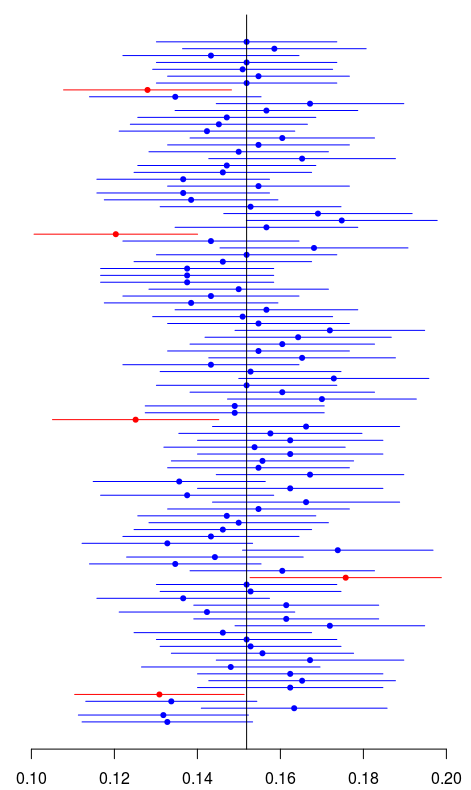
\includegraphics[width=0.55\textwidth]{apendices/imagenes/confidence_interval.png}
        \caption[
            Ejemplo de intervalo de confianza para la media poblacional.
        ]{
            Ejemplo de intervalos de confianza para la media poblacional. La interpretación correcta del nivel de confianza (95\% en este caso) es: \textit{Si repitiéramos el proceso de muestreo y construcción de intervalos muchas veces, aproximadamente el 95\% de ellos contendrían el verdadero valor de la media poblacional}. En esta simulación, la media real conocida es 0.153, y podemos ver que la mayoría de los intervalos la capturan, mientras que unos pocos (generalmente alrededor del 5\%) no lo logran.
            En general, se suele pedir uno solo de estos intervalos, calculado con toda la muestra disponible, aunque la media poblacional podrá estar o no contenida, pero es desconocido. 
        } 
        \label{fig:confidence_interval}
    \end{figure}


    \item El \textbf{intervalo de credibilidad o región creíble (RC)} es, de hecho, la que determina que el parámetro $\theta$ está contenido en el rango de sus valores con una probabilidad determinada por el nivel de credibilidad. Este intervalo es la aproximación bayesiana equivalente al intervalo de confianza, y, como este, requiere conocer la distribución a priori de los datos.

    La diferencia radica en que, a diferencia del intervalo de confianza, que parte de que $\theta$ es un parámetro fijo desconocido y los datos son tratados como aleatorios, el enfoque bayesiano fija los datos(ya que son conocidos) y el parámetro $\theta$ lo trata como aleatorio (ya que es desconocido) \cite{murphy2022}.

    Esta interpretación resulta más intuitiva y directa en comparación con la interpretación frecuentista del intervalo de confianza. En particular, una región creíble del 95\% sí puede interpretarse como que hay un 95\% de probabilidad de que el parámetro $\theta$ se encuentre dentro de ese intervalo, dado el conjunto de datos observado y la distribución a priori asumida.

    \begin{figure}[htbp]
        \centering
        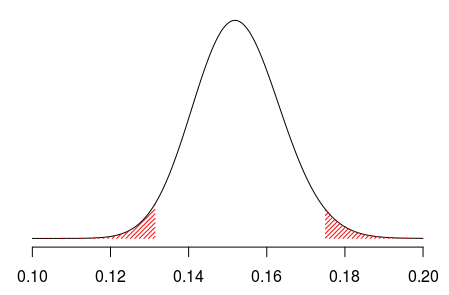
\includegraphics[width=0.75\textwidth]{apendices/imagenes/credibility_interval.png}
        \caption[
            Ejemplo de intervalo de credibilidad para la media poblacional.
        ]{
            Ejemplo de intervalo de credibilidad para la media poblacional. La interpretación correcta es: \textit{Con un 95\% de probabilidad, el valor verdadero está dentro del intervalo}. En esta simulación, la media real conocida es 0.153, y podemos observar que efectivamente este valor está contenido en el intervalo.
        } 
        \label{fig:credibility_interval}
    \end{figure}


    \item El \textbf{intervalo de predicción (\textit{prediction interval})} es radicalmente diferente a los intervalos previos. Trata de predecir un valor futuro de una observación, no determinar un parámetro poblacional. Existen numerosos métodos, con y sin necesidad de conocer la distribución de los datos. 
    
    El enfoque explorado en este trabajo es la predicción conformal, que ha demostrado ser eficaz en contextos donde los supuestos clásicos (normalidad, homocedasticidad) no se cumplen \cite{romano2019}, y es actualmente el enfoque más robusto para la construcción de intervalos de predicción en aplicaciones modernas de ML \cite{romano2019, luo2025, sadinle2019, romano2020, angelopoulos2020}. La predicción conformal tiene una interpretación frecuentista: $1-\alpha$ intervalos producidos cubren el verdadero valor (véase la Figura \ref{fig:prediction_intervals}).

    \begin{figure}[htbp]
        \centering
        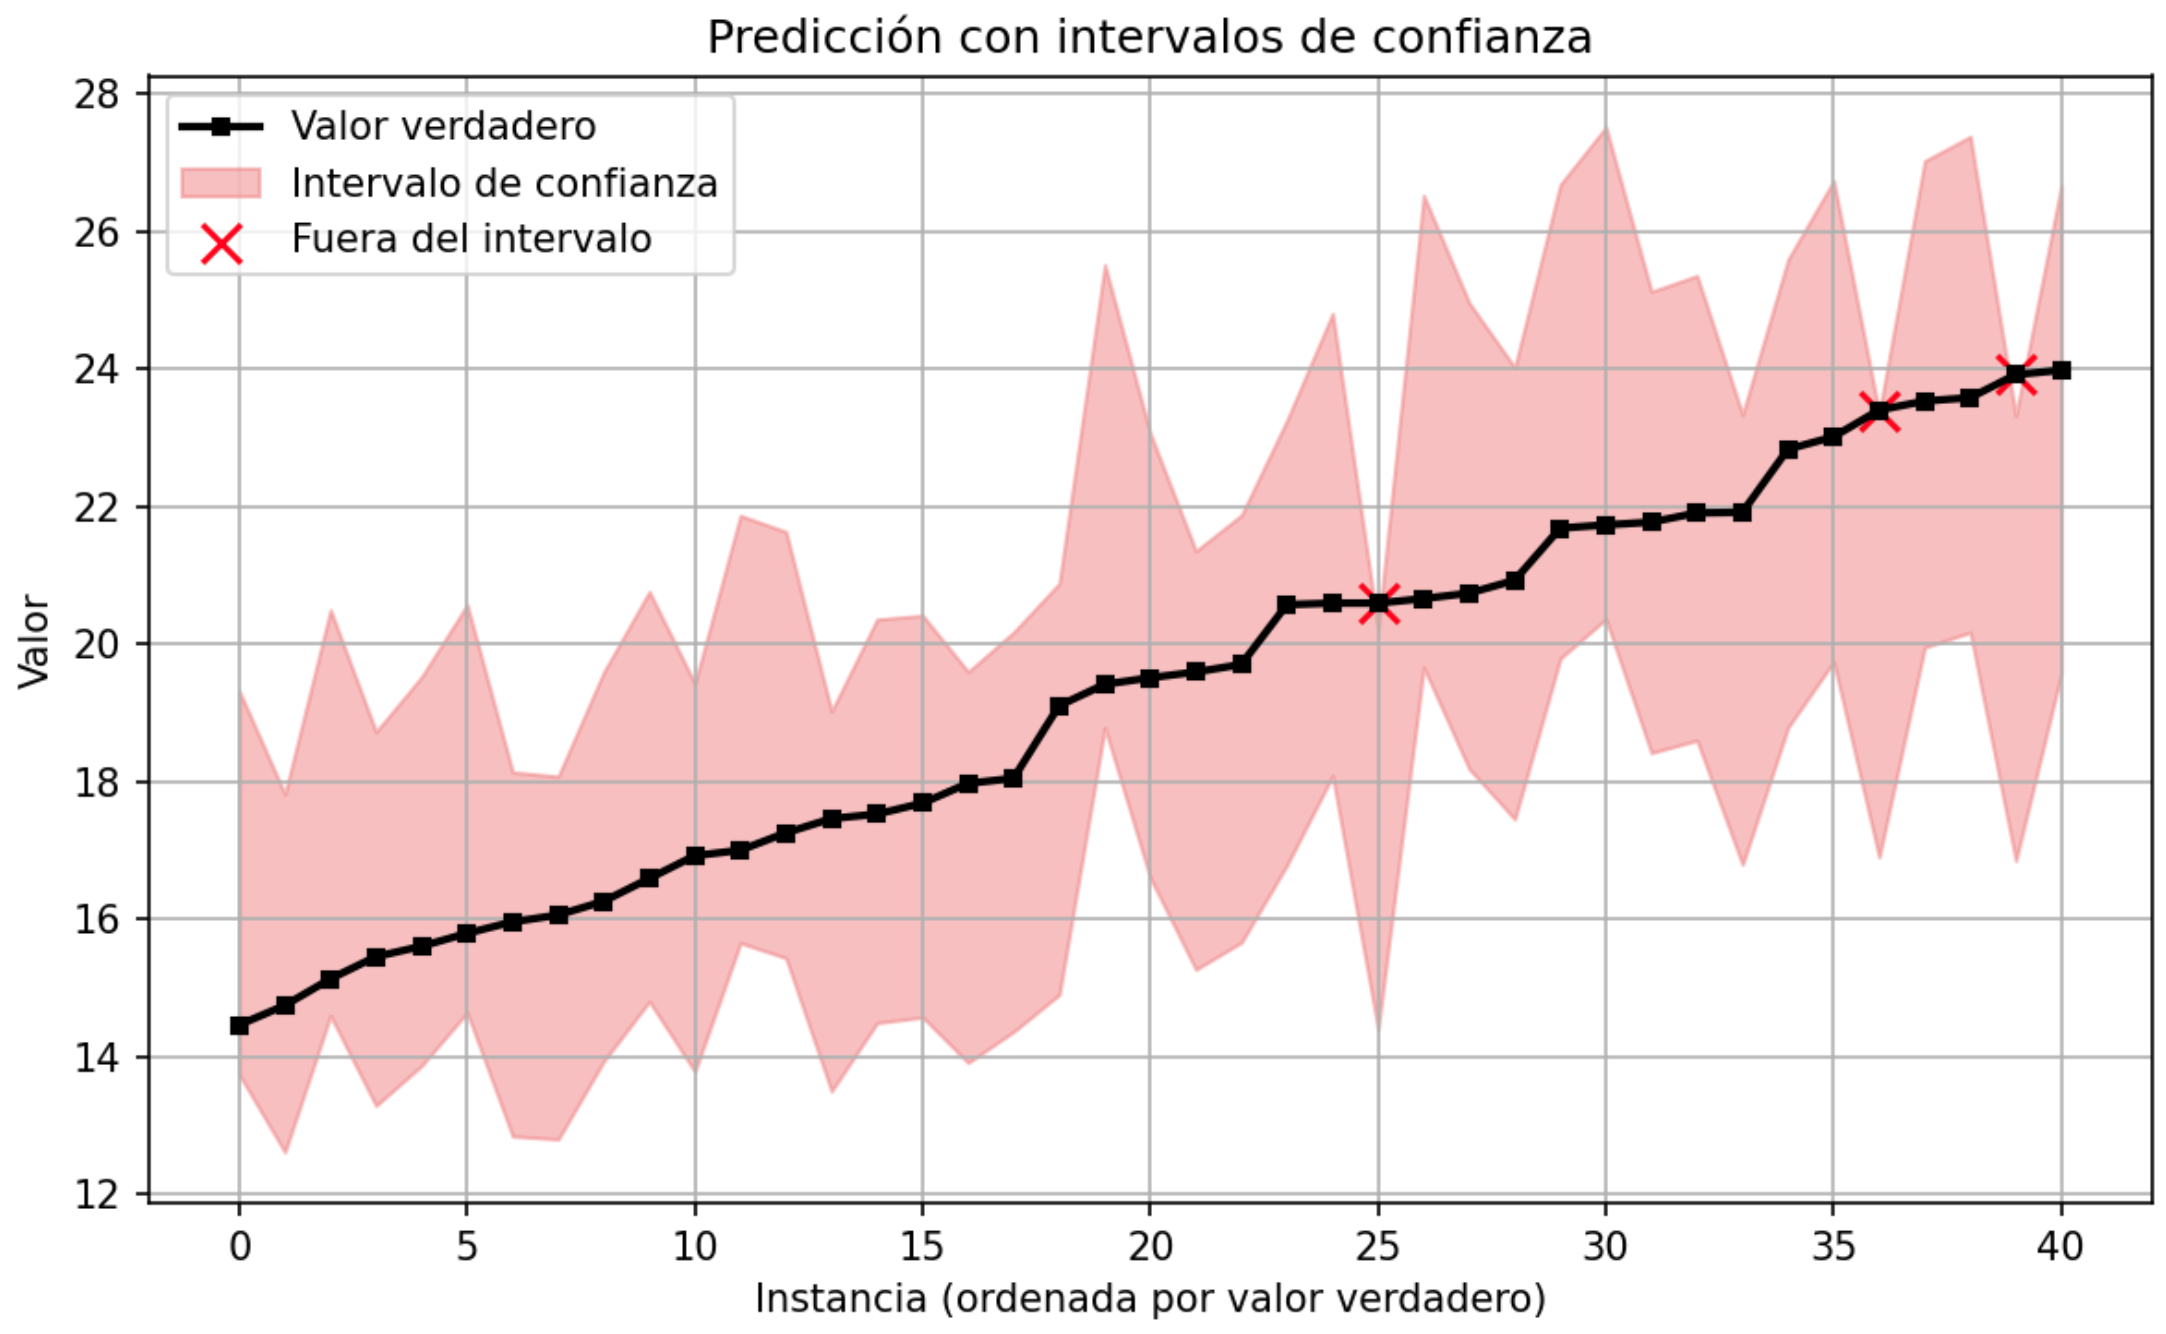
\includegraphics[width=0.75\textwidth]{apendices/imagenes/prediction_intervals.png}
        \caption[
            Intervalos de predicción (95\% de confianza) construidos con CQR para estimación de edad.
        ]{
            Intervalos de predicción (95\% de confianza) construidos con CQR para estimación de edad.
        } 
        \label{fig:prediction_intervals}
    \end{figure}

\end{itemize}

% Relacionándolo con el apartado anterior, los intervalos de confianza solo informan de la incertidumbre 
% aleatoria, puesto que asumen que el modelo está bien especificado y que el error residual es la única fuente 
% de variabilidad. 

% Los intervalos de credibilidad sí integran la incertidumbre en los parámetros del modelo y en la estructura 
% del modelo mismo, capturando así tanto la incertidumbre aleatoria como la incertidumbre epistémica.

% Frente a estos, los intervalos de predicción obtenidos mediante predicción conformal sí presentan información
% de los tres componentes de incertidumbre. 

Como podemos esperar, a más estrecho sea el intervalo que manejemos, más se puede confiar en las predicciones pero no todos los tipos de intervalos revelan la misma información sobre incertidumbre. 

   %\chapter{Identificación genética}

En este también se recomienda la identificación genética como técnica que ofrece más garantías de fiabilidad y 
precisión en los procesos de identificación humana, destacando la importancia de establecer una base de datos nacional 
de ADN que permita cruzar información genética. Además, enfatiza la necesidad de contar con laboratorios especializados 
en genética forense, dotados de tecnología avanzada y personal cualificado, debido a los desafíos técnicos que presenta 
la degradación del ADN en los restos exhumados y la posible contaminación de las muestras

Este trabajo se centra en la estimación del perfil biológico (edad, sexo, estatura) más que en la identificación 
humana, por lo que no abordará análisis genéticos. No obstante, el estudio osteológico mantiene su relevancia por 
varias razones:

\begin{enumerate}
    
    \item La concentración de ADN se reduce drásticamente en los primeros 8 meses post-mortem \cite{higgins2015differential}. 
    Y factores como las altas temperaturas, la exposición a humedad ambiental o la presencia de aguas subterraneas y 
    entornos ricos en oxígeno, que fomentan la presencia microbiana, perjudican la conservación del ADN 
    \cite{latham2018dna}. 

    Además, a parte de la degradación, el ADN puede sufrir contaminación, tanto por microorganismos presentes en el entorno 
    del cadáver, como por restos óseos de otros individuos.

    % Separar el ADN de dos humanos es imposible en este tipo de situaciones. 

    %Un análisis realizado a partir de 15 informes involucrando a 933 cadáveres exhumados en el Cementerio de Paterna, 
    %Valencia, determinó en 149 las identificaciones exitosas, suponiendo un 15,9 \% de individuos identificados.

    \item Se necesitan muestras con las que comparar las secuencias de ADN extraída de los individuos, a ser posible de
    familiares de primer grado. 


    \item El proceso genético para la identificación es costoso, especialmente si son muchas las muestras a cruzar. 
    Una estimación previa del perfil biológico podría facilitar la identificación, pudiendo comparar el ADN con una base
    de datos más pequeña.

\end{enumerate}

   %\input{apendices/manual_usuario/manual_usuario}
   %%\input{apendices/paper/paper}
   %\input{glosario/entradas_glosario}
   % \addcontentsline{toc}{chapter}{Glosario}
   % \printglossary
   \chapter*{}
   \thispagestyle{empty}

\end{document}
